\documentclass[11pt]{report}

% For including image file
\usepackage{graphicx, color}

% For including collection of image
%\usepackage{subcaption}

% For generating hyper links

% For coloring text
\usepackage{xcolor}

%\usepackage{hyperref}
\usepackage[linkbordercolor=white, colorlinks=true, urlcolor=black, linkcolor=black]{hyperref}

% Margin of the page
\usepackage[top=0.5in, bottom=1in, left=1in, right=1in]{geometry}

%For adding nomenclature
%\usepackage{nomencl}
%\makenomenclature
%\renewcommand{\nomname}{Annotation}

% For cover page tikz image 
%\usepackage{tikz}
%\usetikzlibrary{calc}

% For including a piece of code
%\usepackage{listings}

% Images folder
%\graphicspath{{Images/}}

\usepackage{titlesec}

\titleformat{\chapter}[display]
{\normalfont\Large\filcenter\sffamily}
{\vspace*{\fill}
 \titlerule[1pt]%
 \vspace{1pt}%
 \titlerule
 \vspace{1pc}%
 \LARGE\MakeUppercase{\chaptertitlename}~\thechapter}
{1pc}
{\titlerule\Huge}
[\vspace*{\fill}\newpage]

\titlespacing*{\chapter}{0pt}{0pt}{0pt}

\titleformat{name=\chapter,numberless}[display]
{\normalfont\Large\filcenter\sffamily}
{}
{0pt}
{\titlerule[1pt]\Huge}
[\titlerule]

\usepackage{pdfpages}

\begin{document}

\tableofcontents

\chapter{Introduction to ROS and its Package Management}
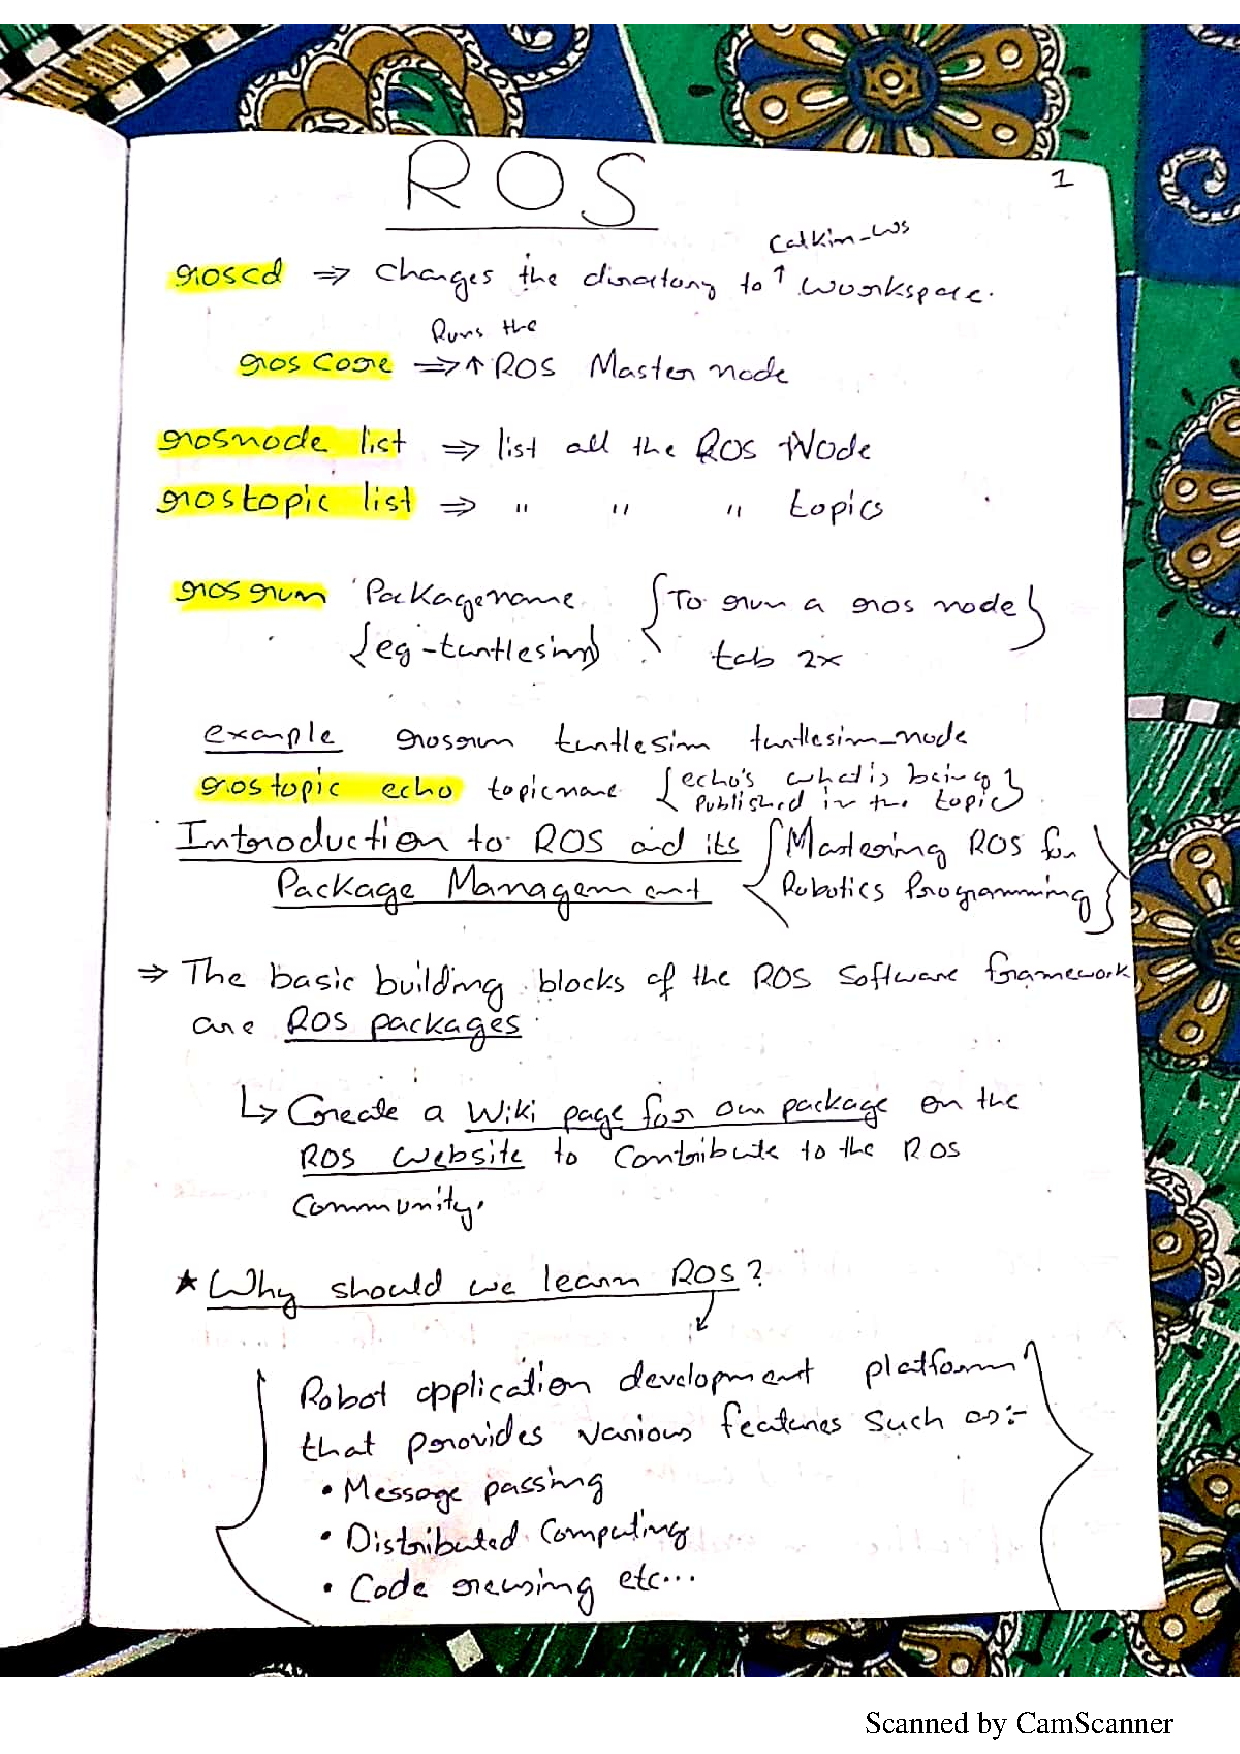
\includepdf[page=-]{./raw_files/1.pdf}

\chapter{ROS Official Tutorial}
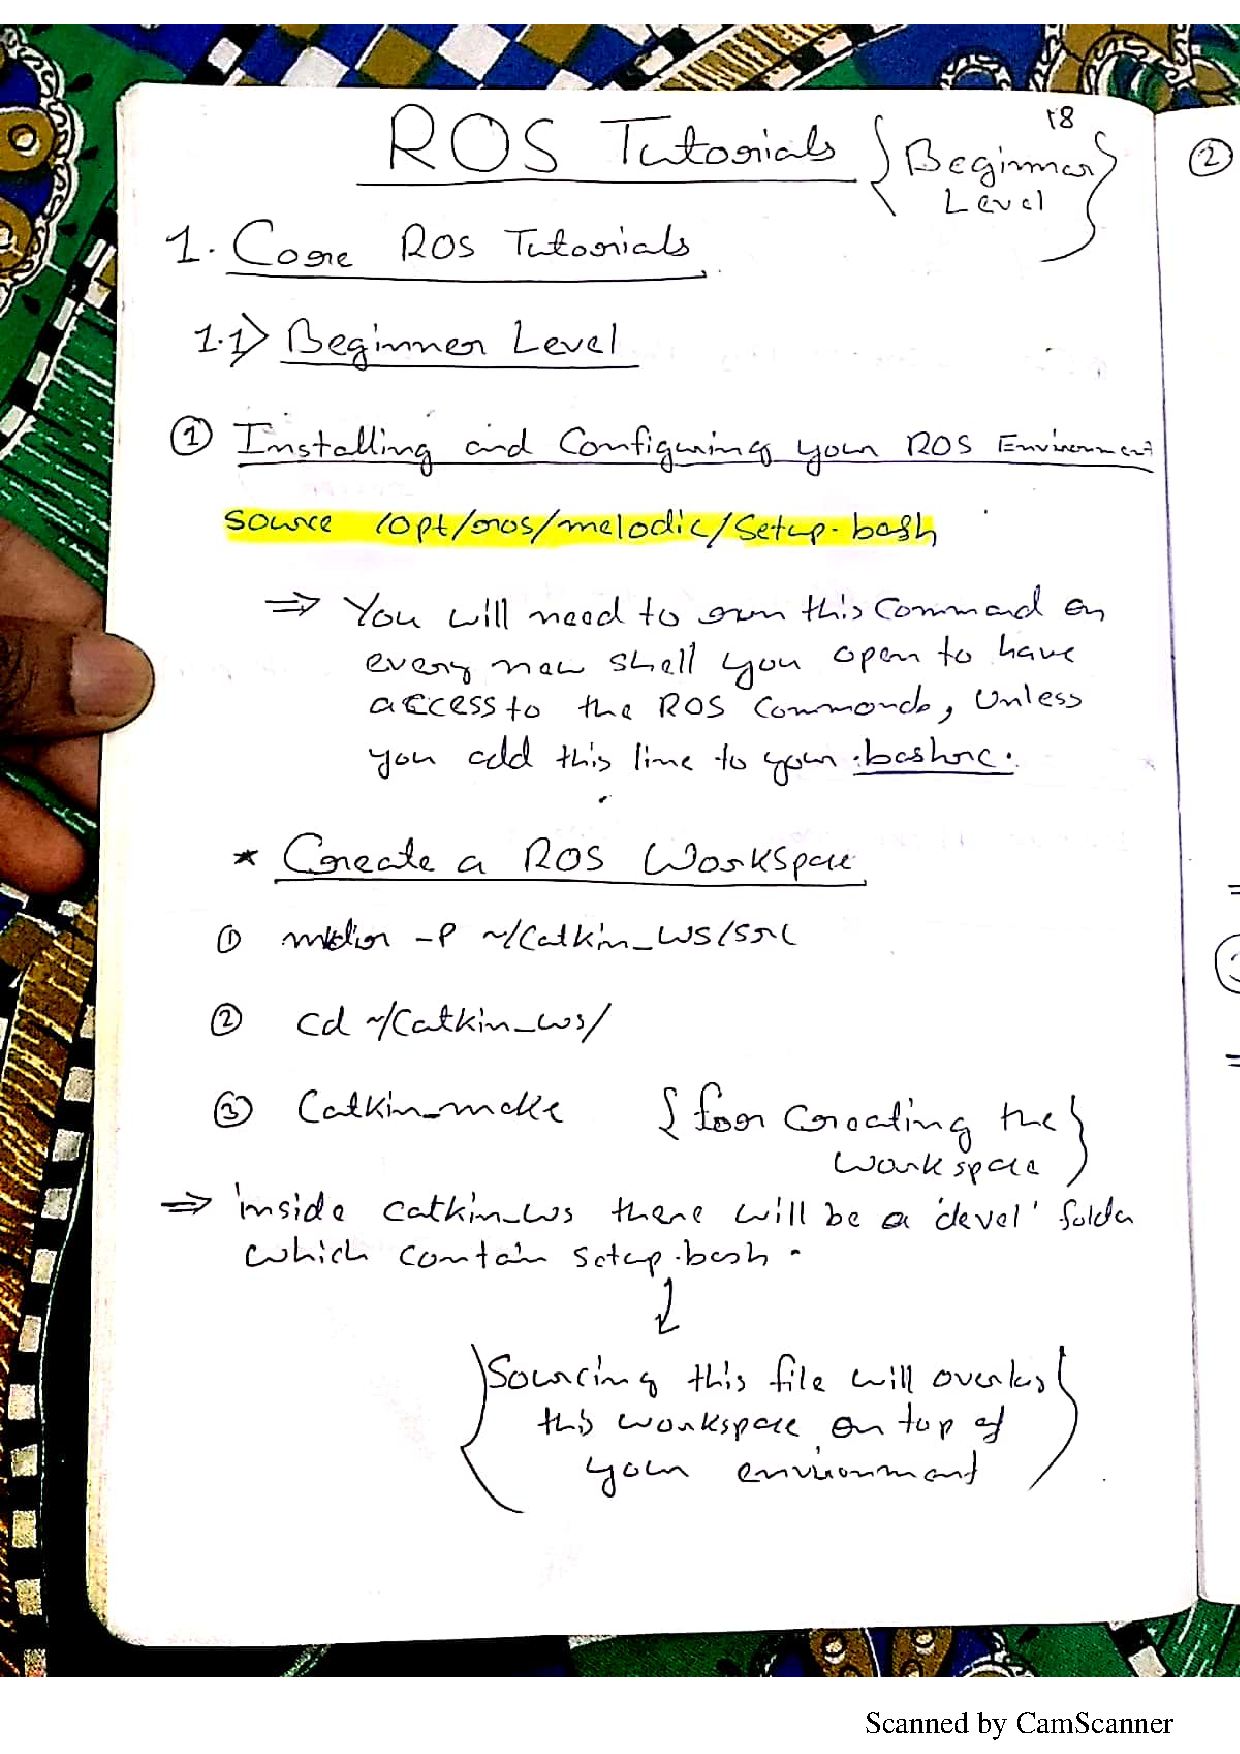
\includepdf[page=-]{./raw_files/2.pdf}

\chapter{ETH zuric cource}
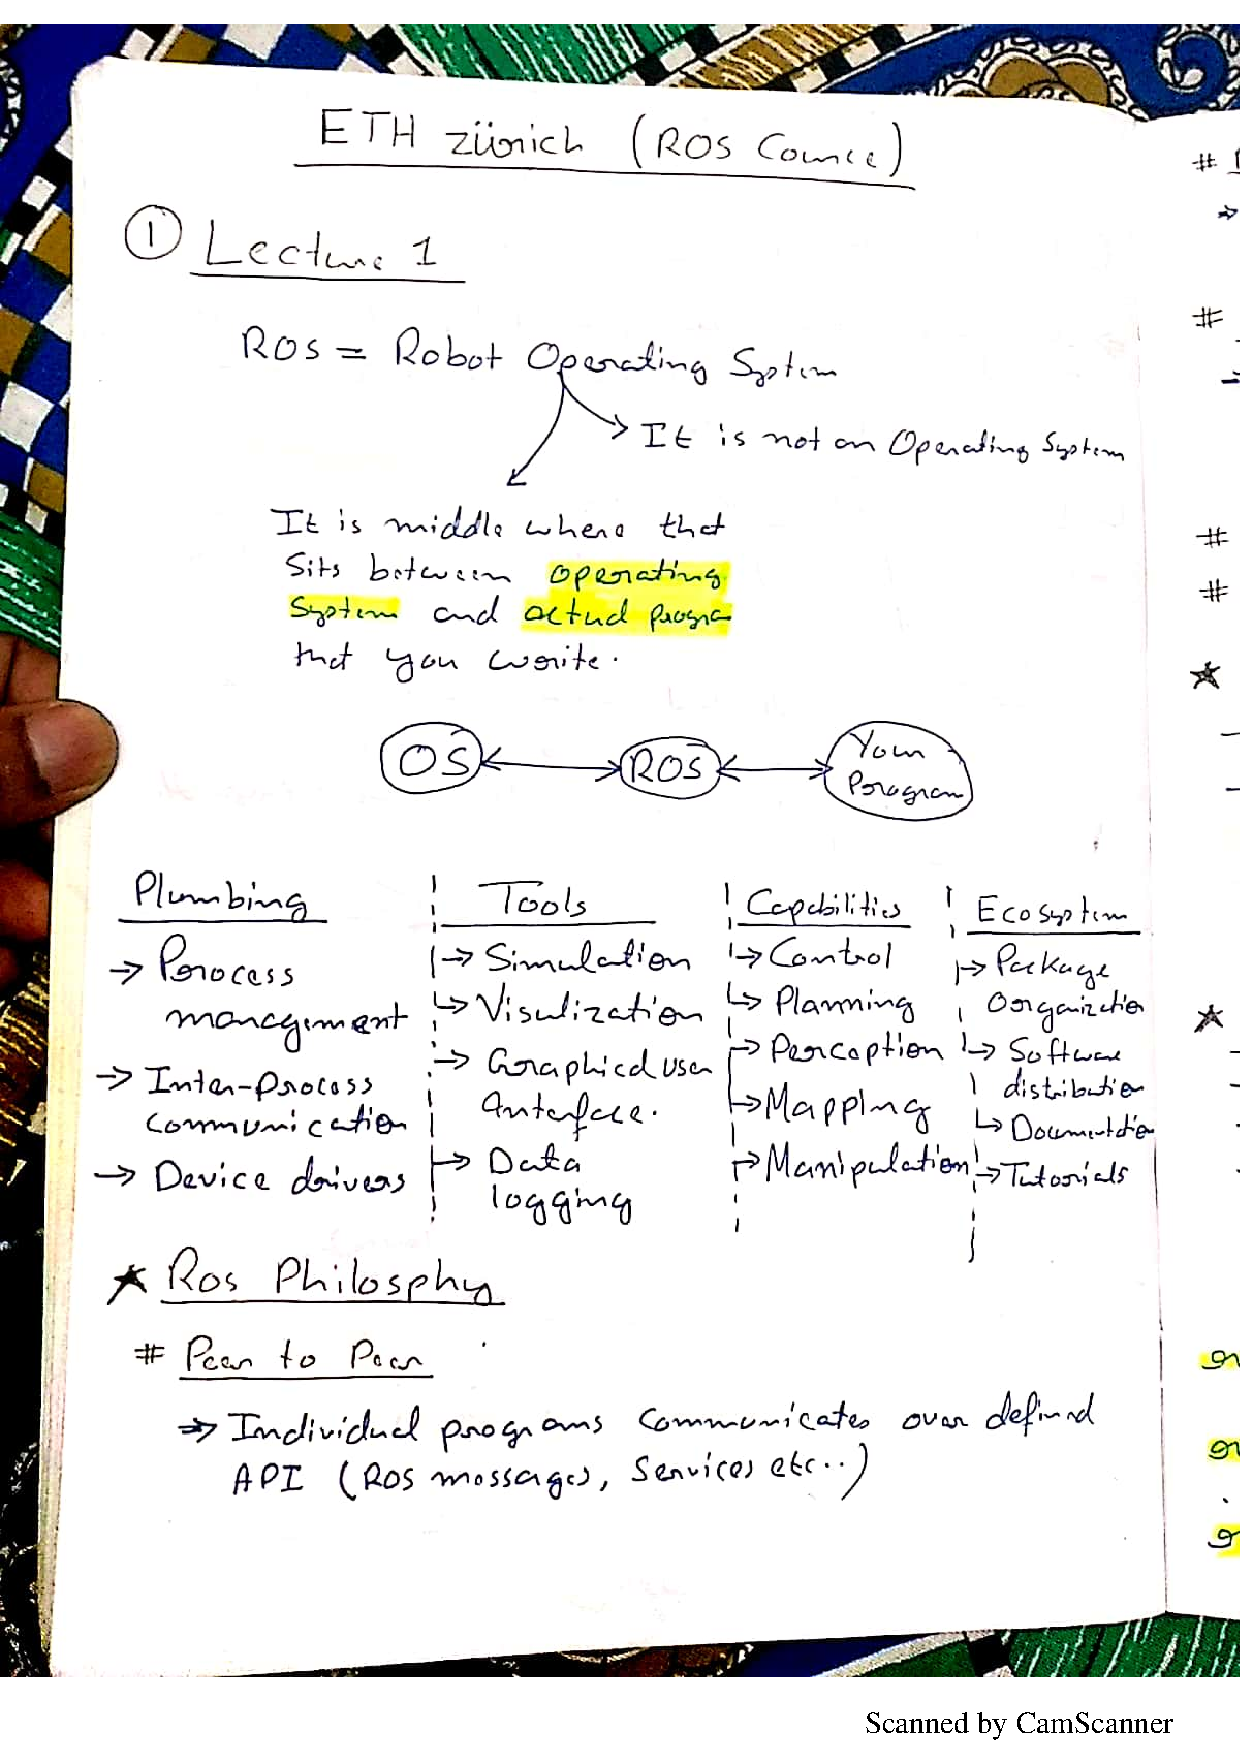
\includepdf[page=-]{./raw_files/3.pdf}

\chapter{TF Turorial}
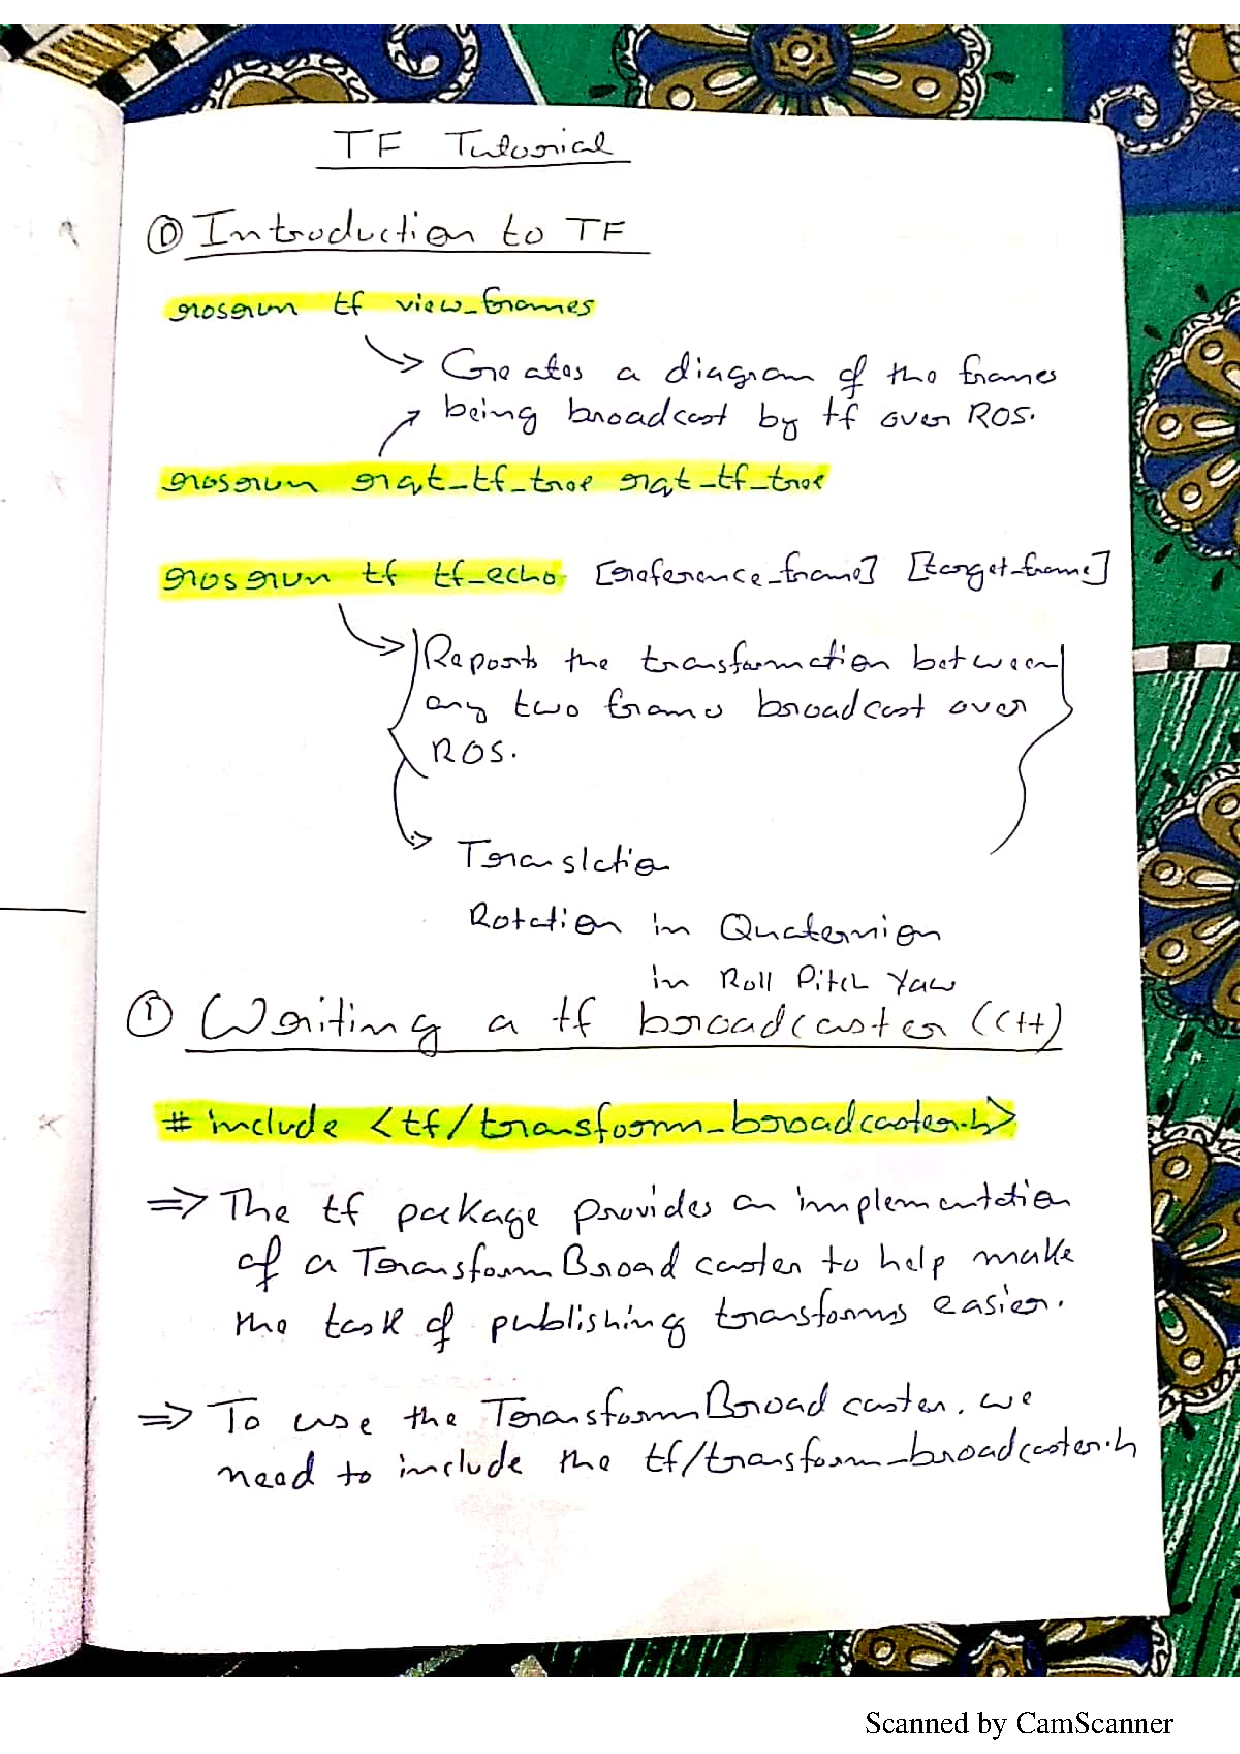
\includepdf[page=-]{./raw_files/4.pdf}

\chapter{URDF Tutorial}
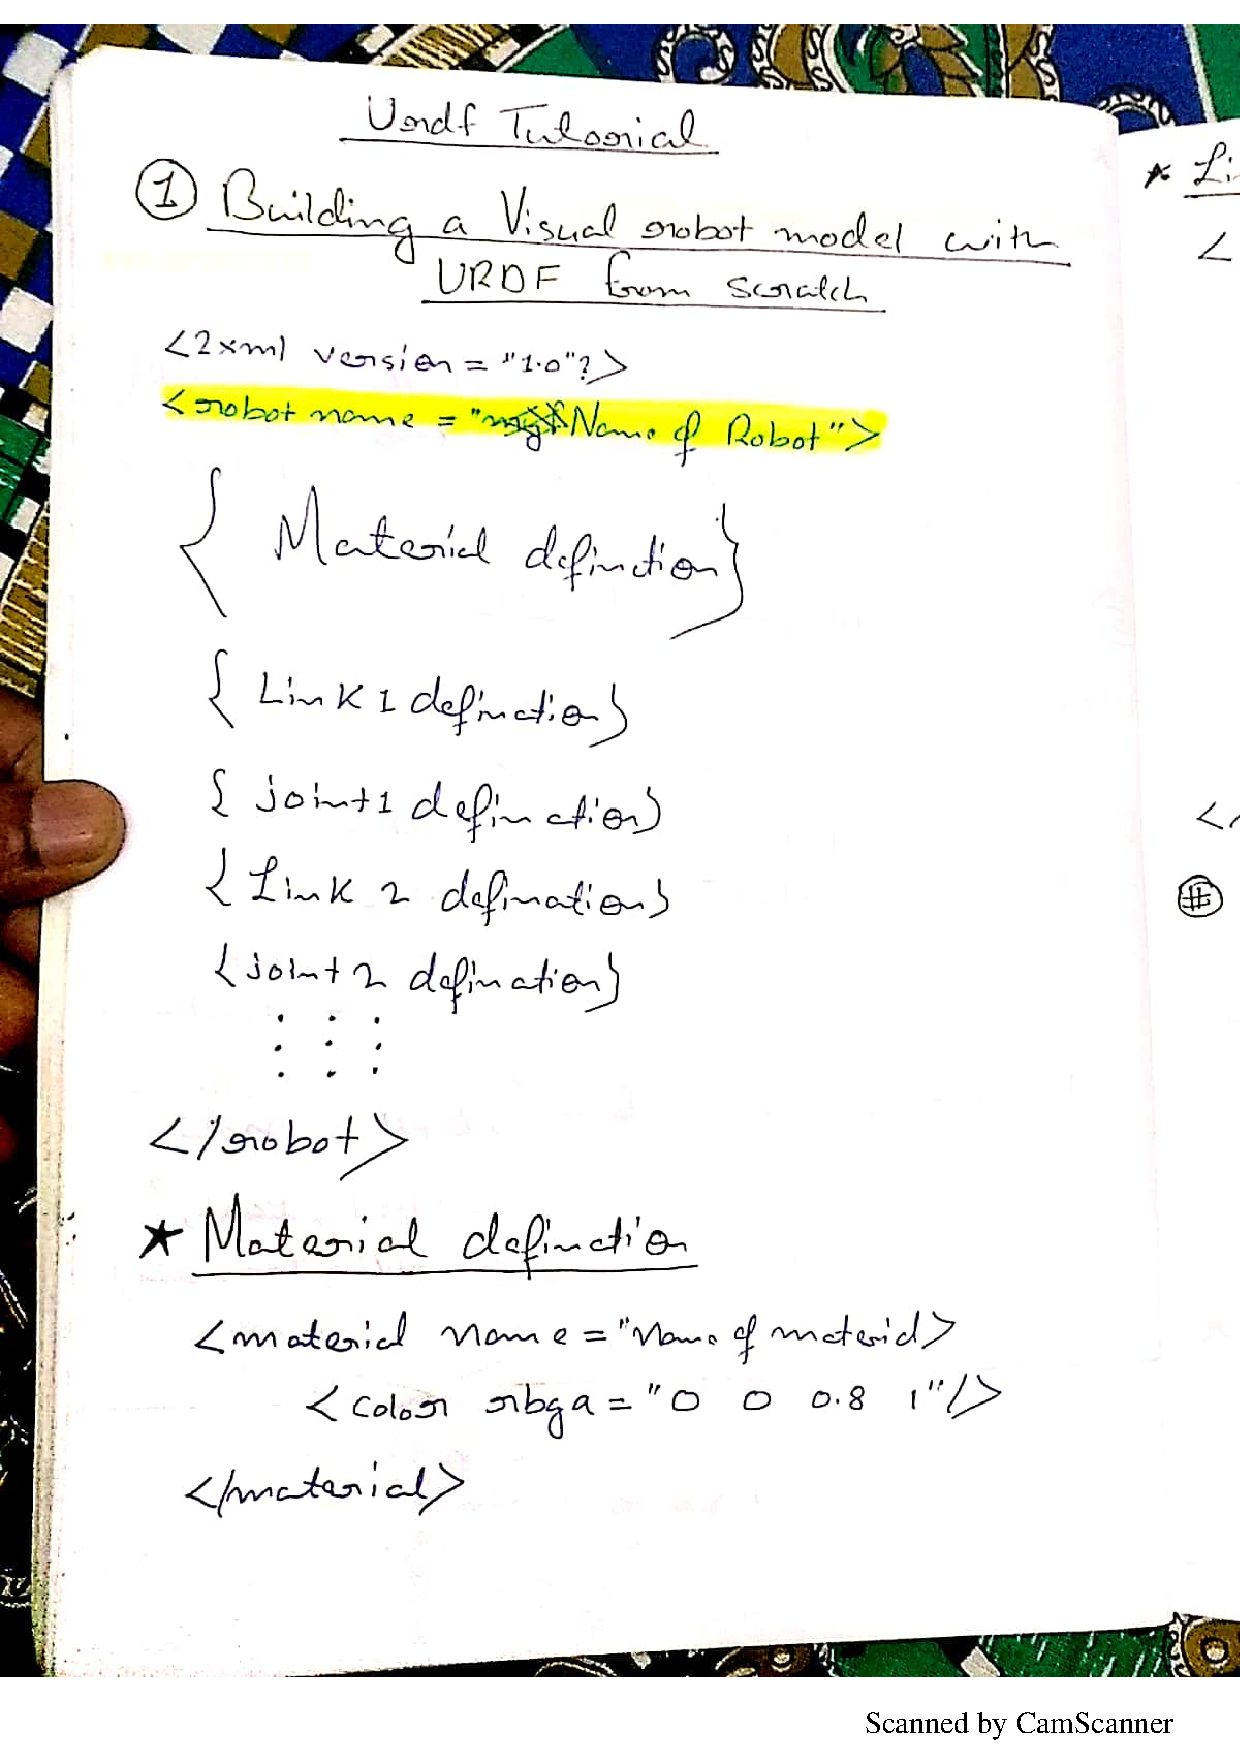
\includepdf[page=-]{./raw_files/5.pdf}

\chapter{Mastering ROS for Robotics Program}
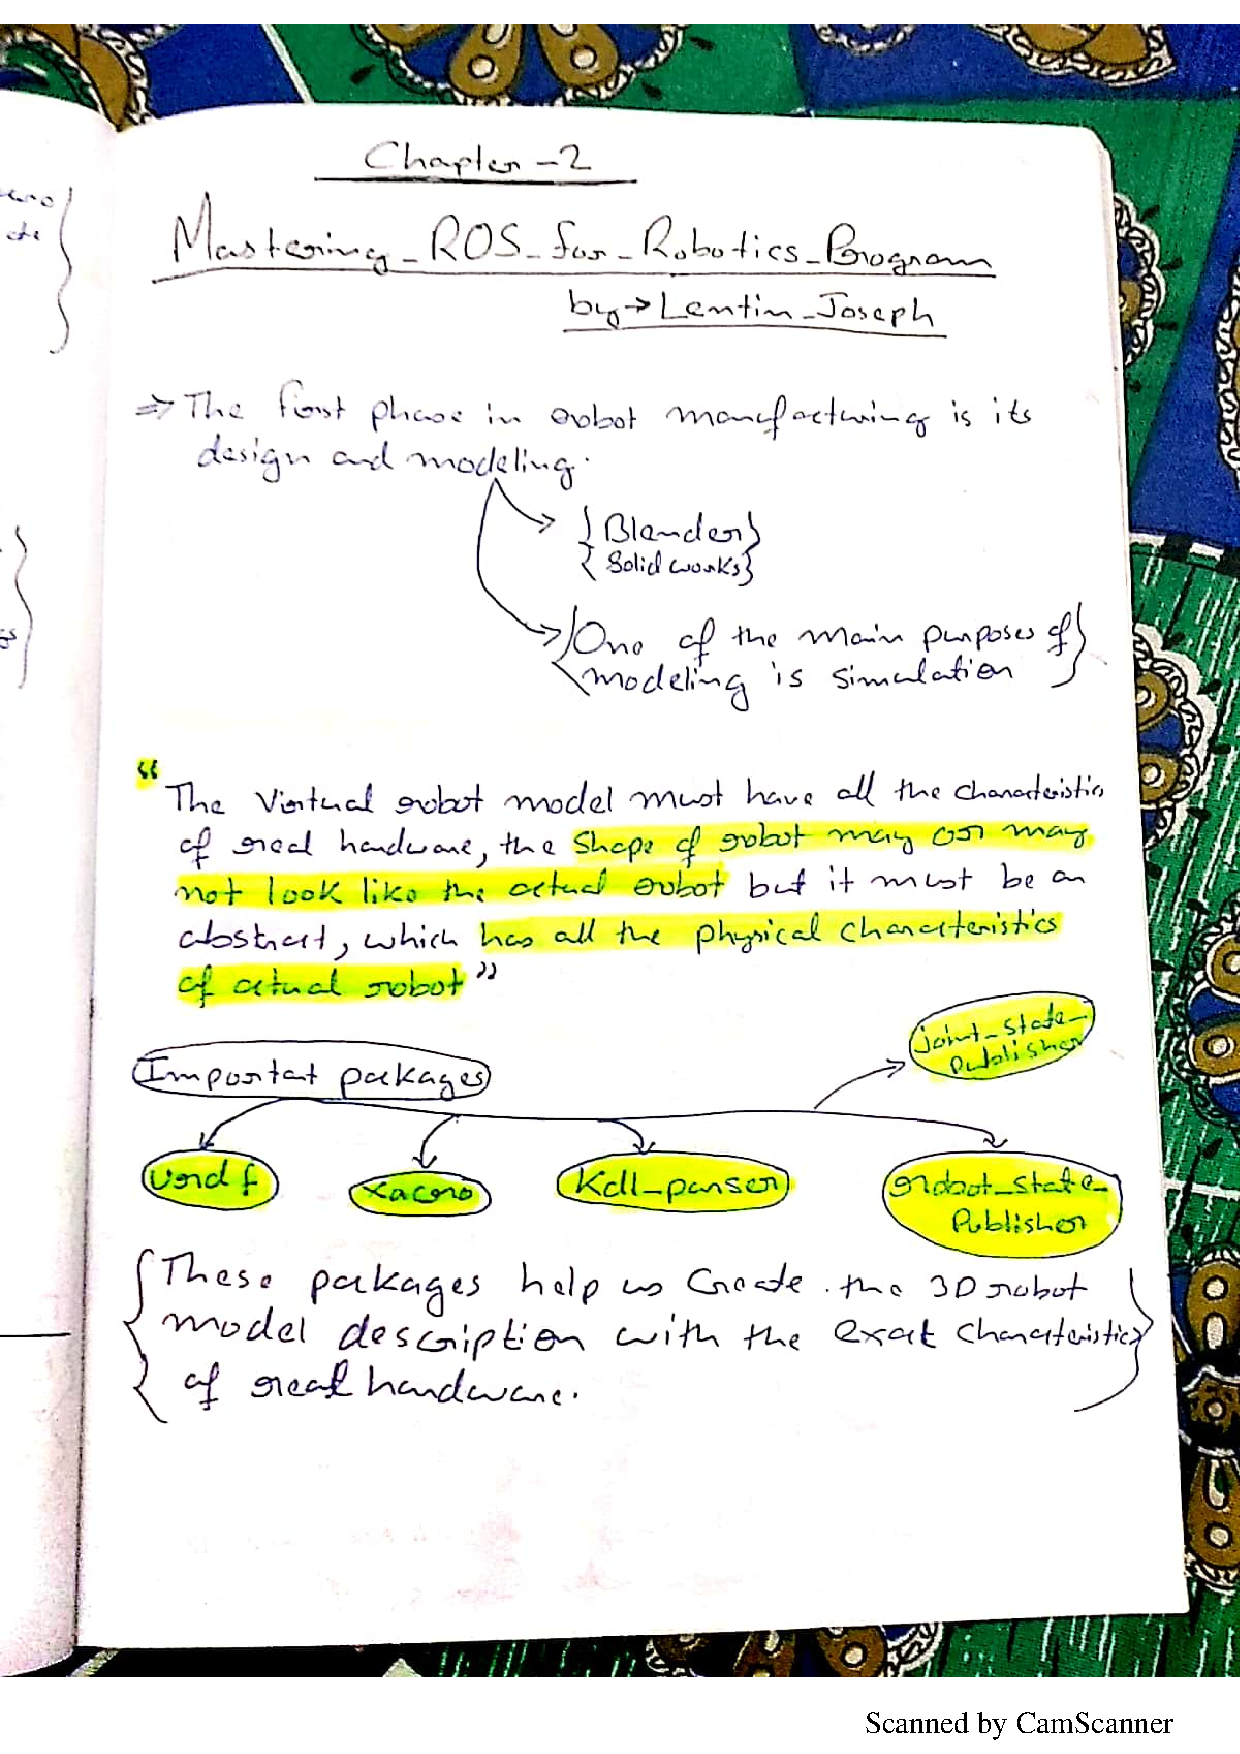
\includepdf[page=-]{./raw_files/6.pdf}

\chapter{Simulating Robot Using ROS and Gazebo}
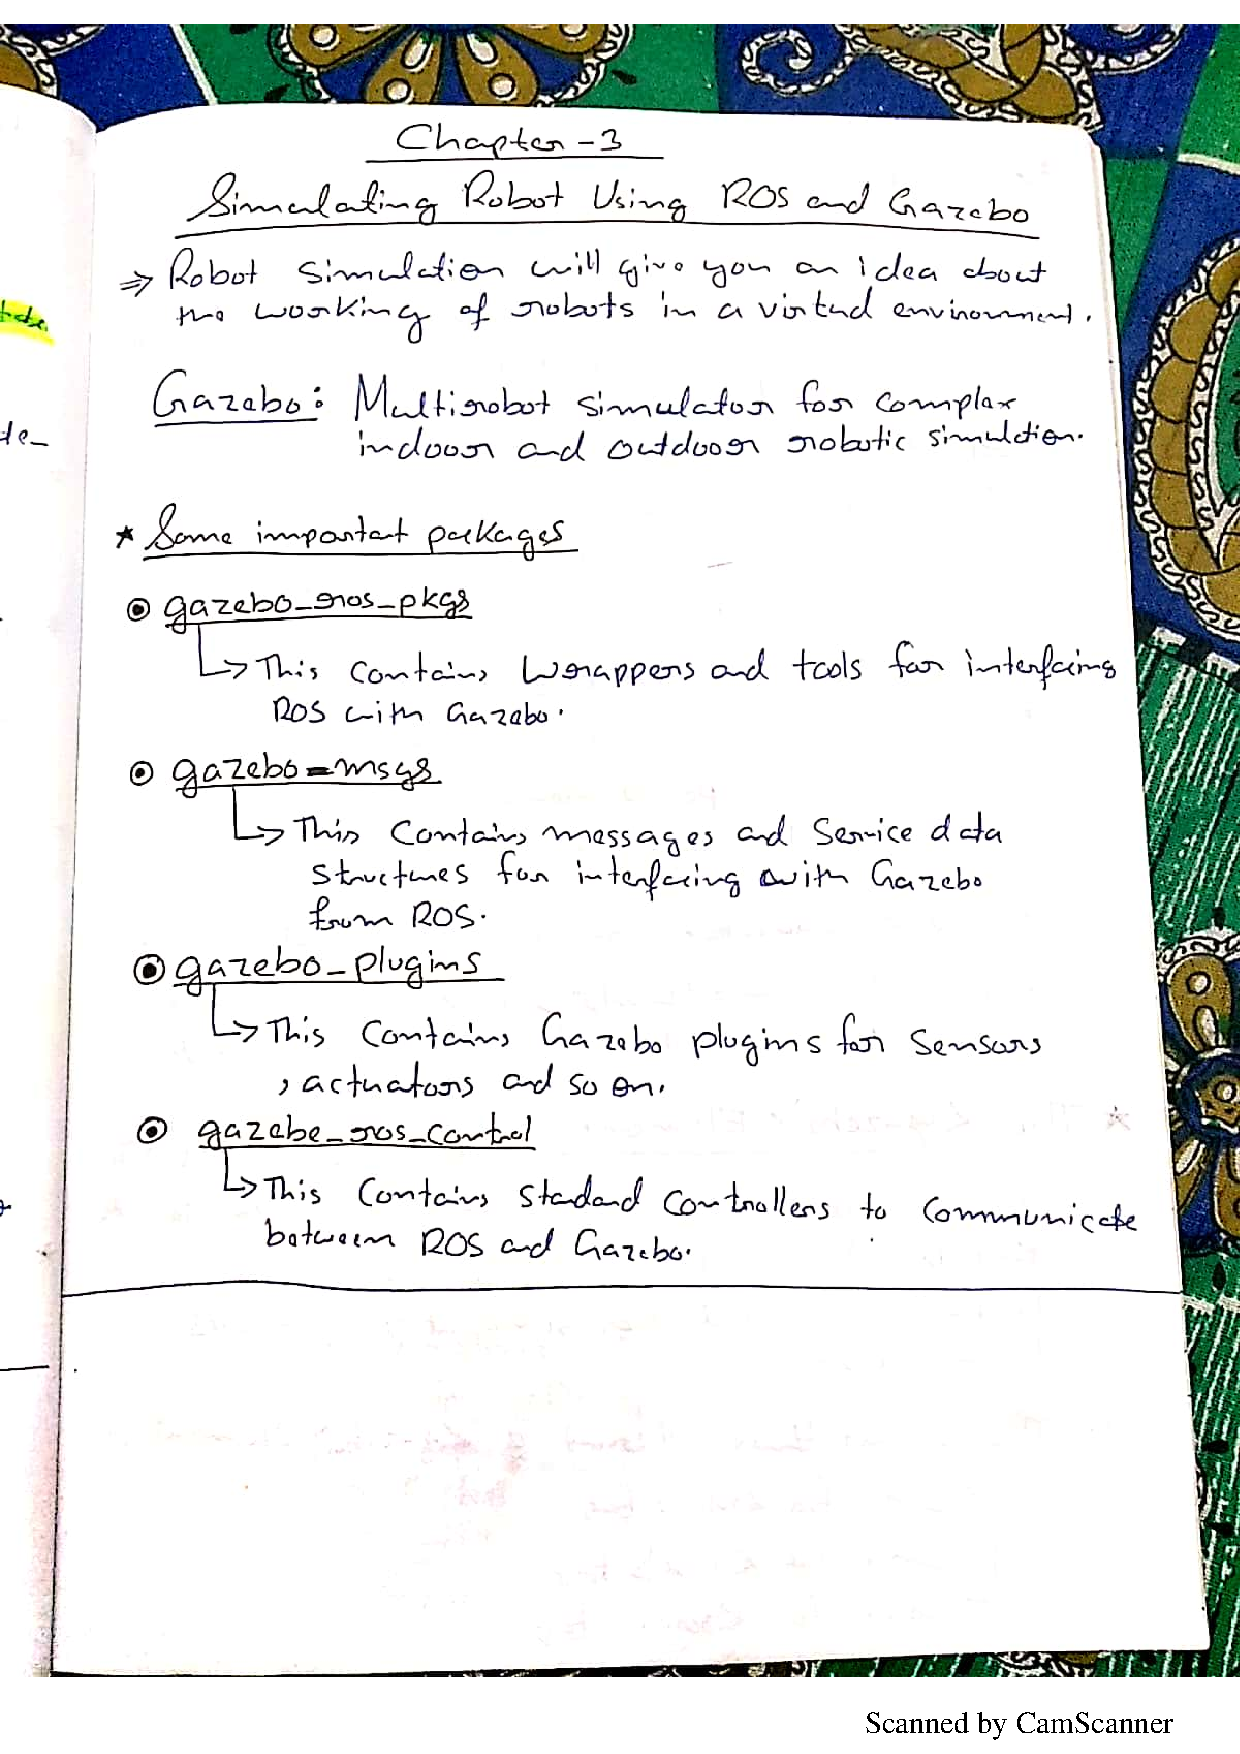
\includepdf[page=-]{./raw_files/7.pdf}

\chapter{ROS Controllers}
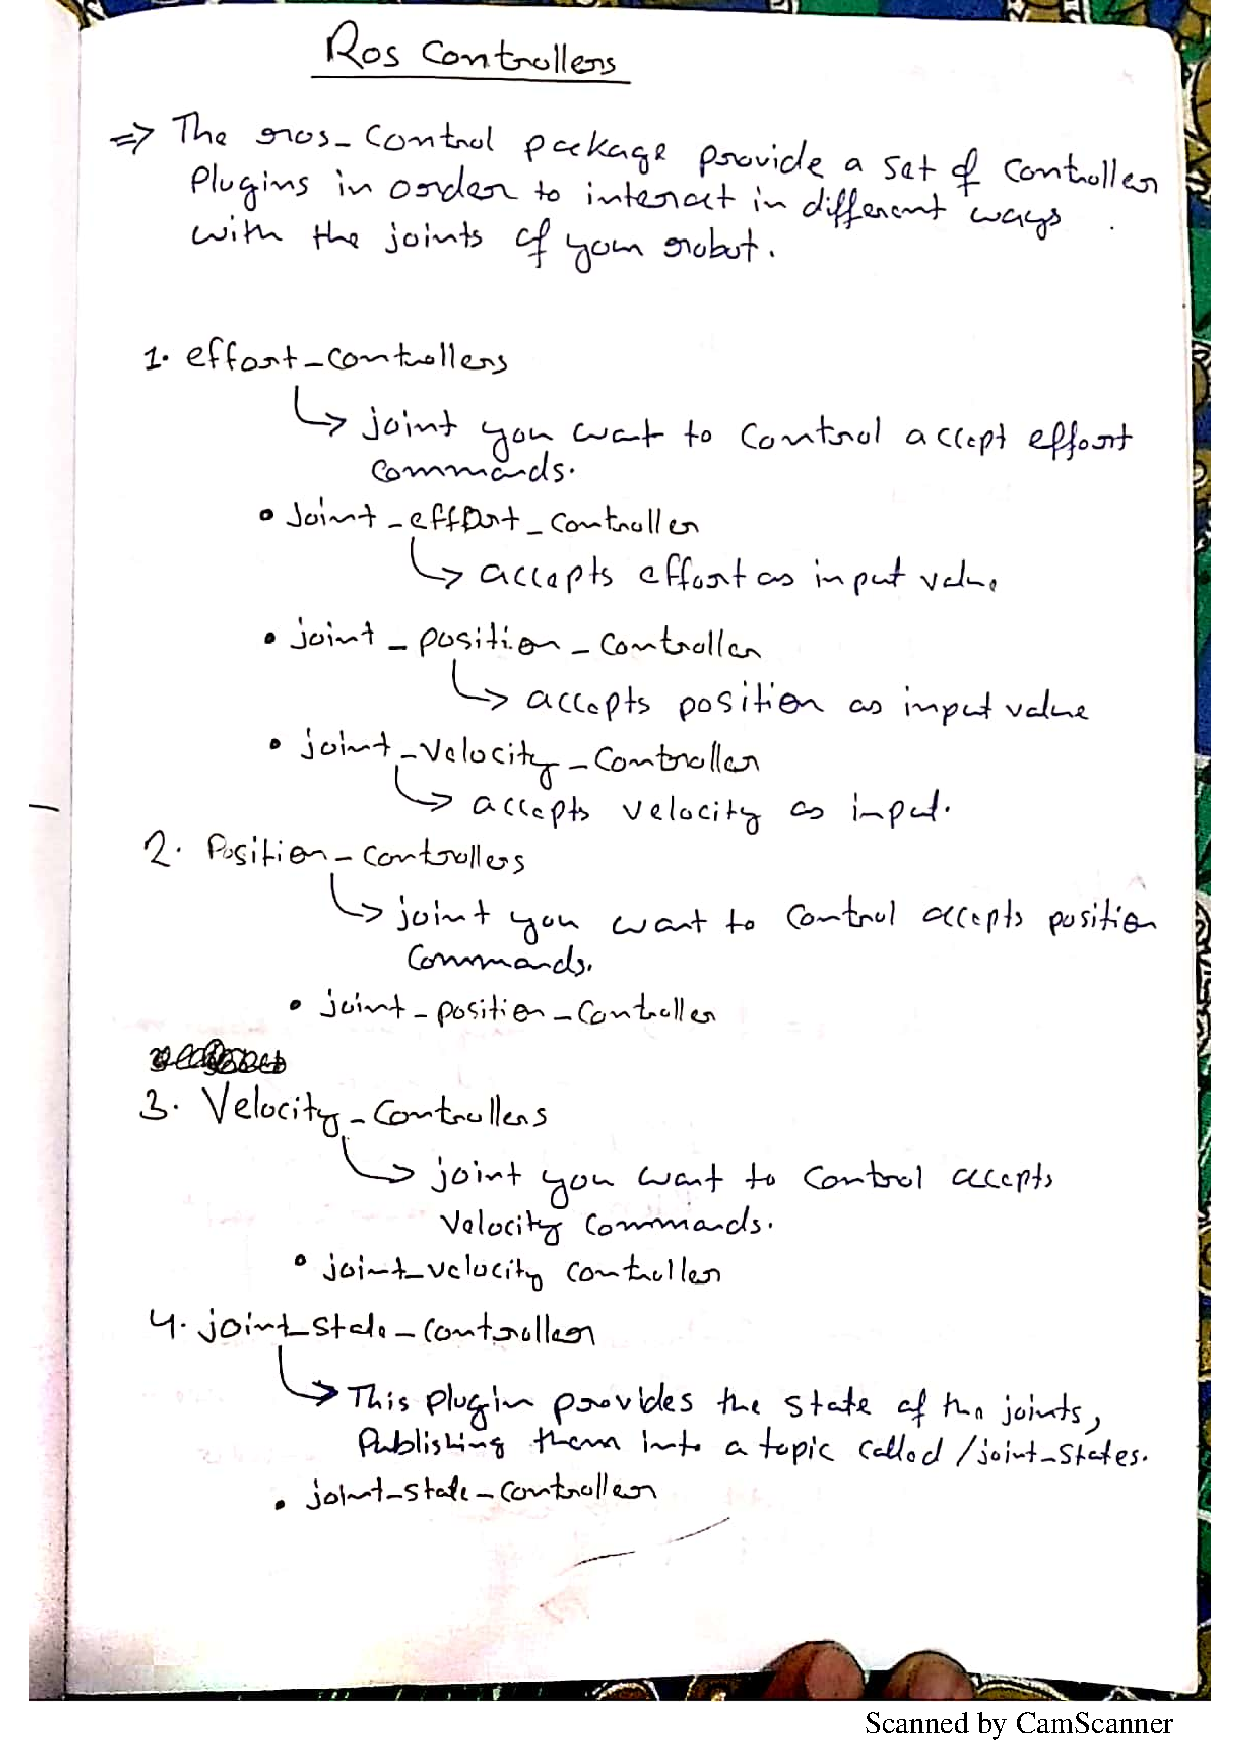
\includepdf[page=-]{./raw_files/8.pdf}

\chapter{Navigation Stack}
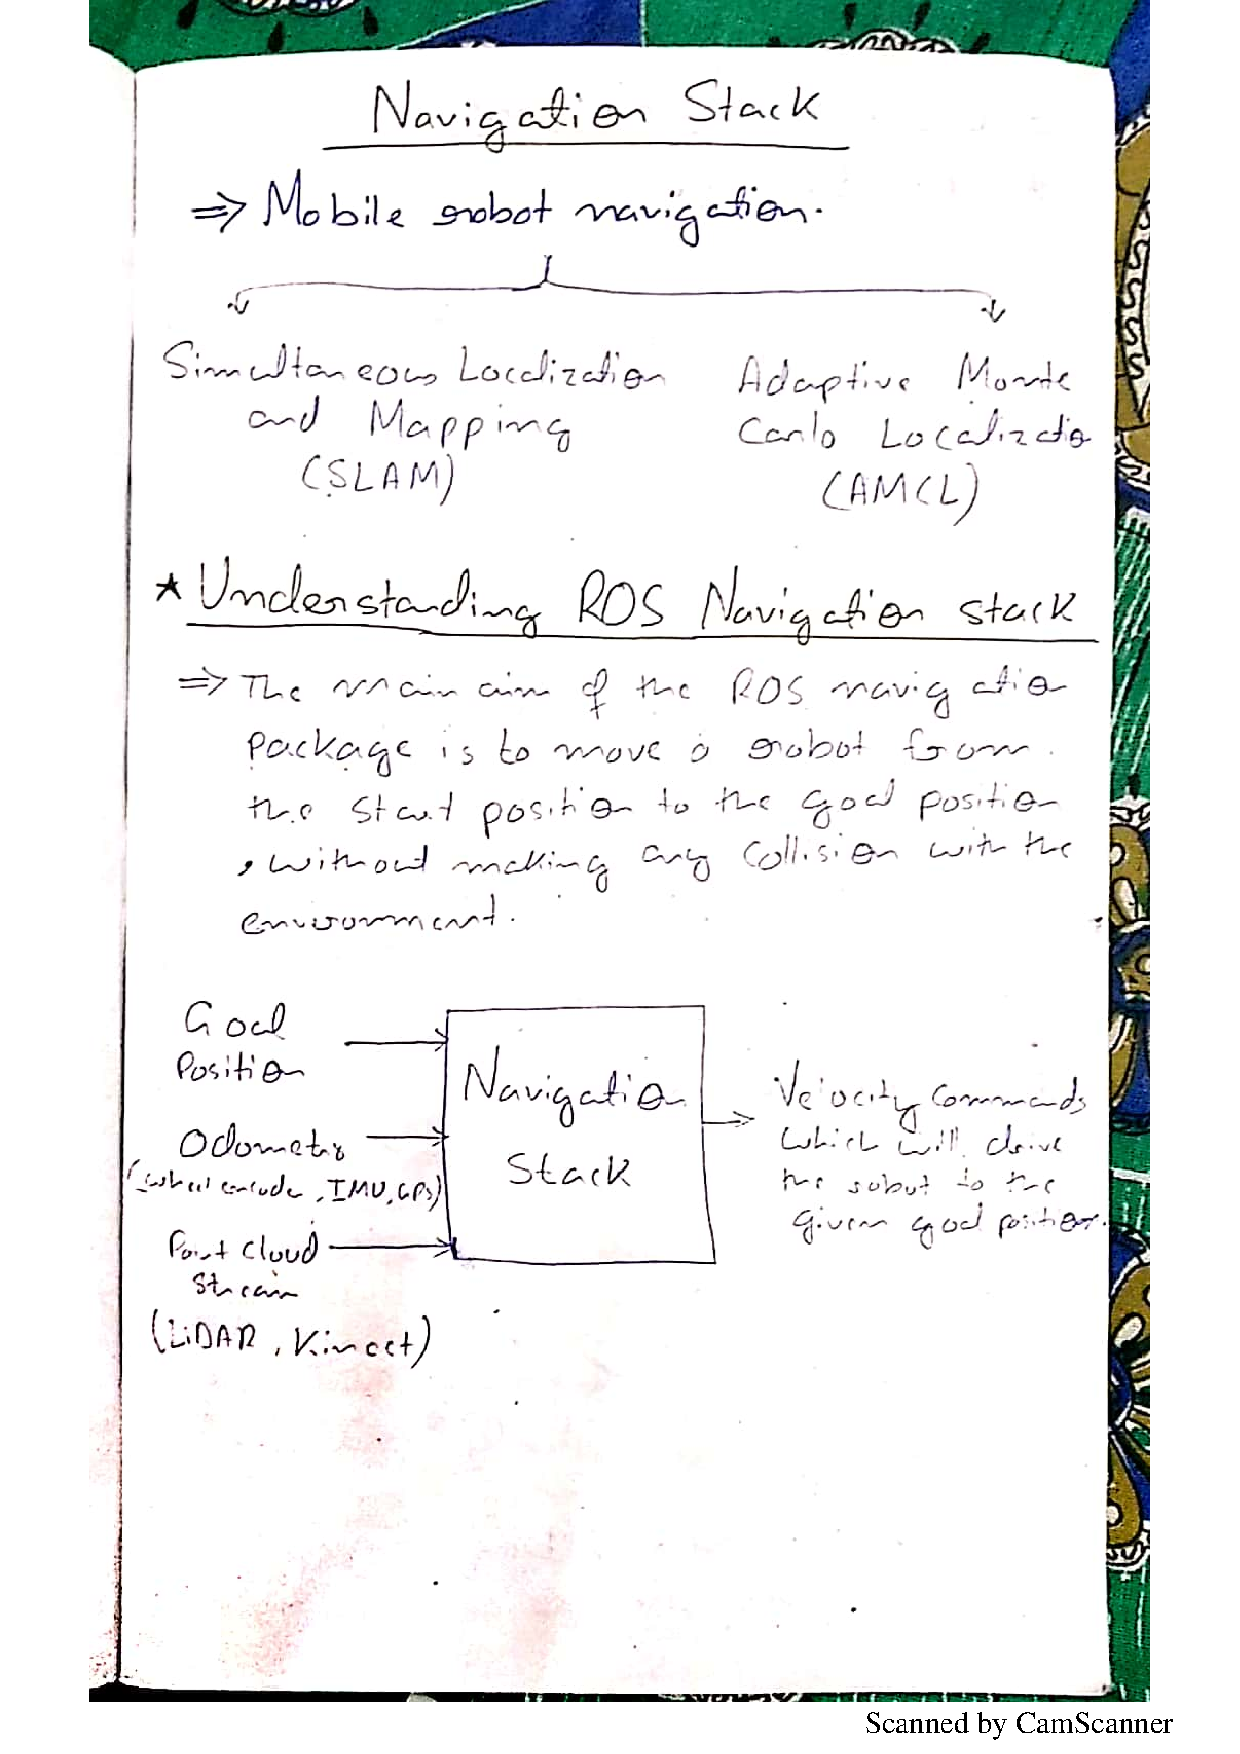
\includepdf[page=-]{./raw_files/9.pdf}

\chapter{Interfacing I/O Board, Sensor, and Actuators to ROS}
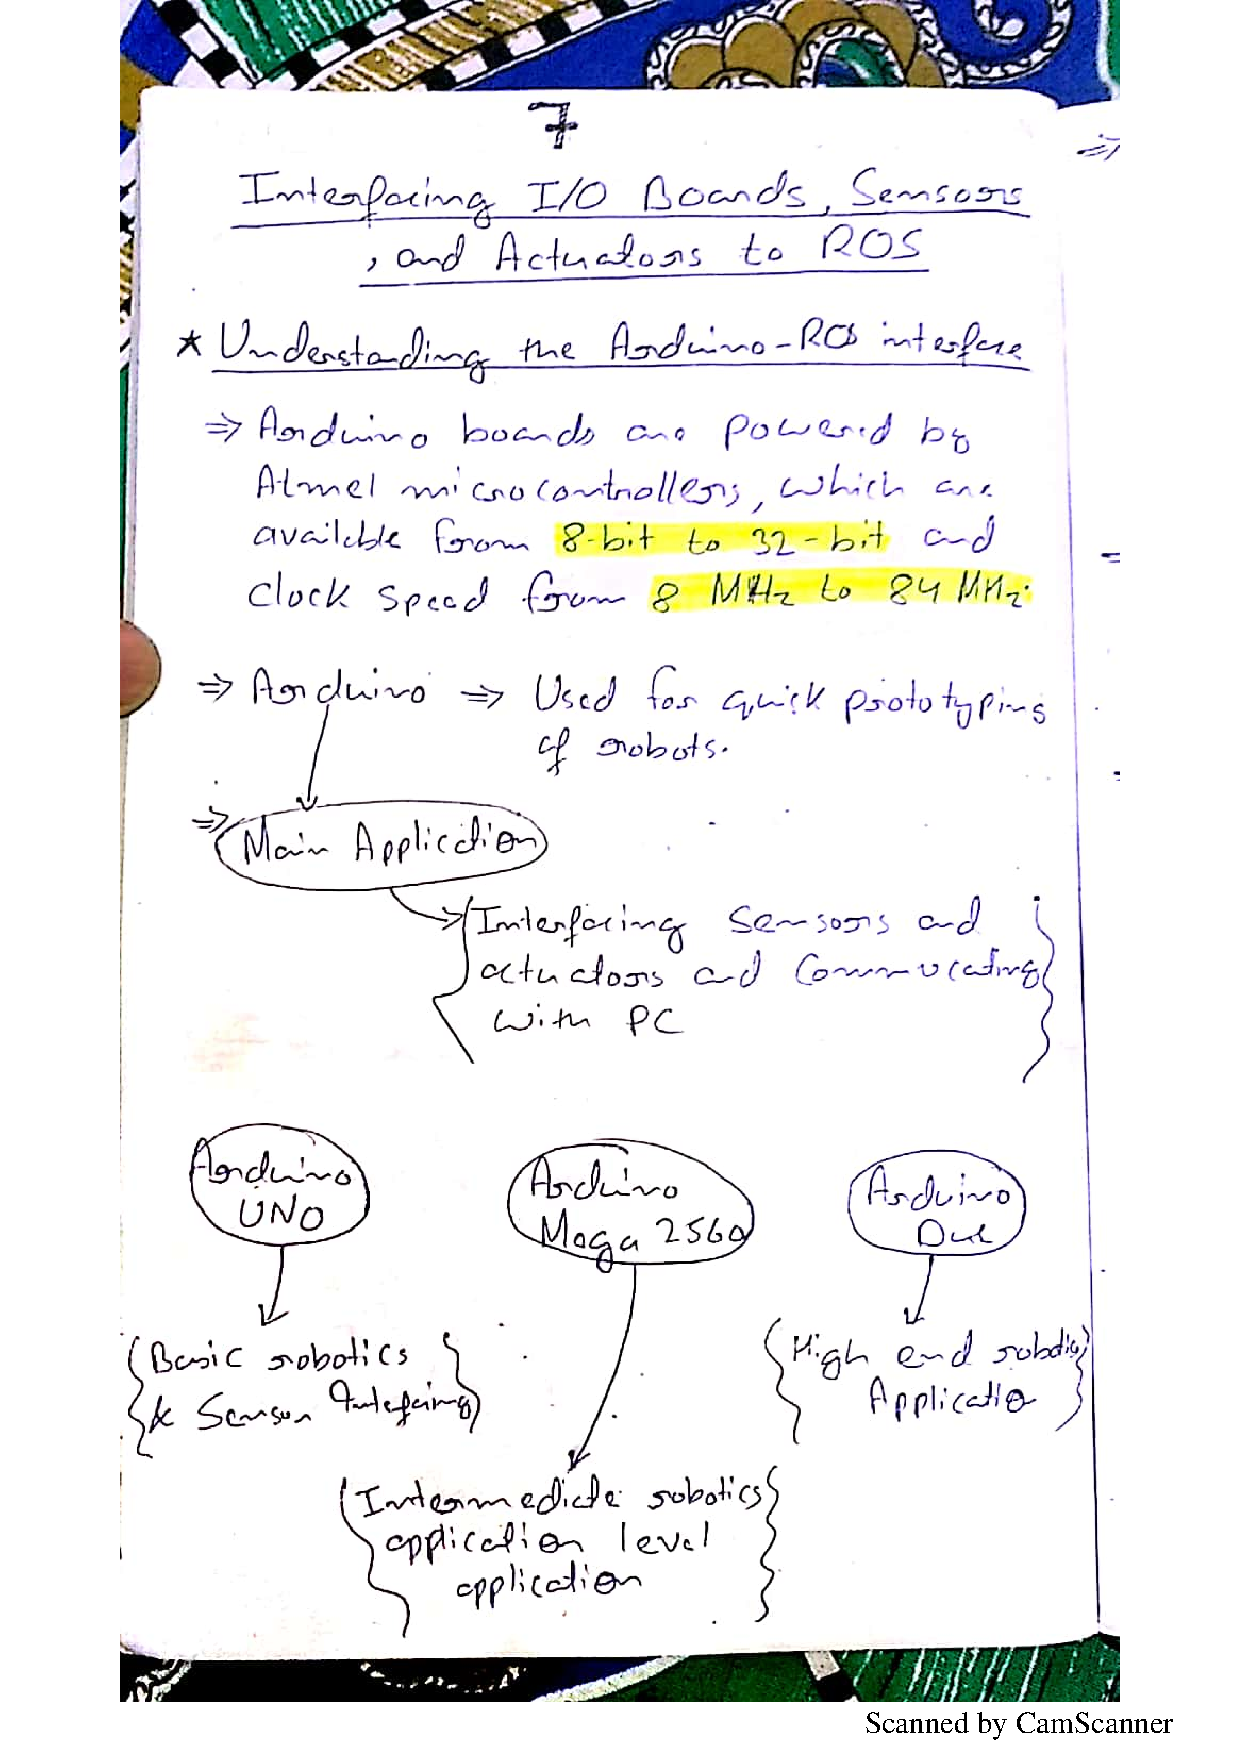
\includepdf[page=-]{./raw_files/10.pdf}

\chapter{ROS Tools}
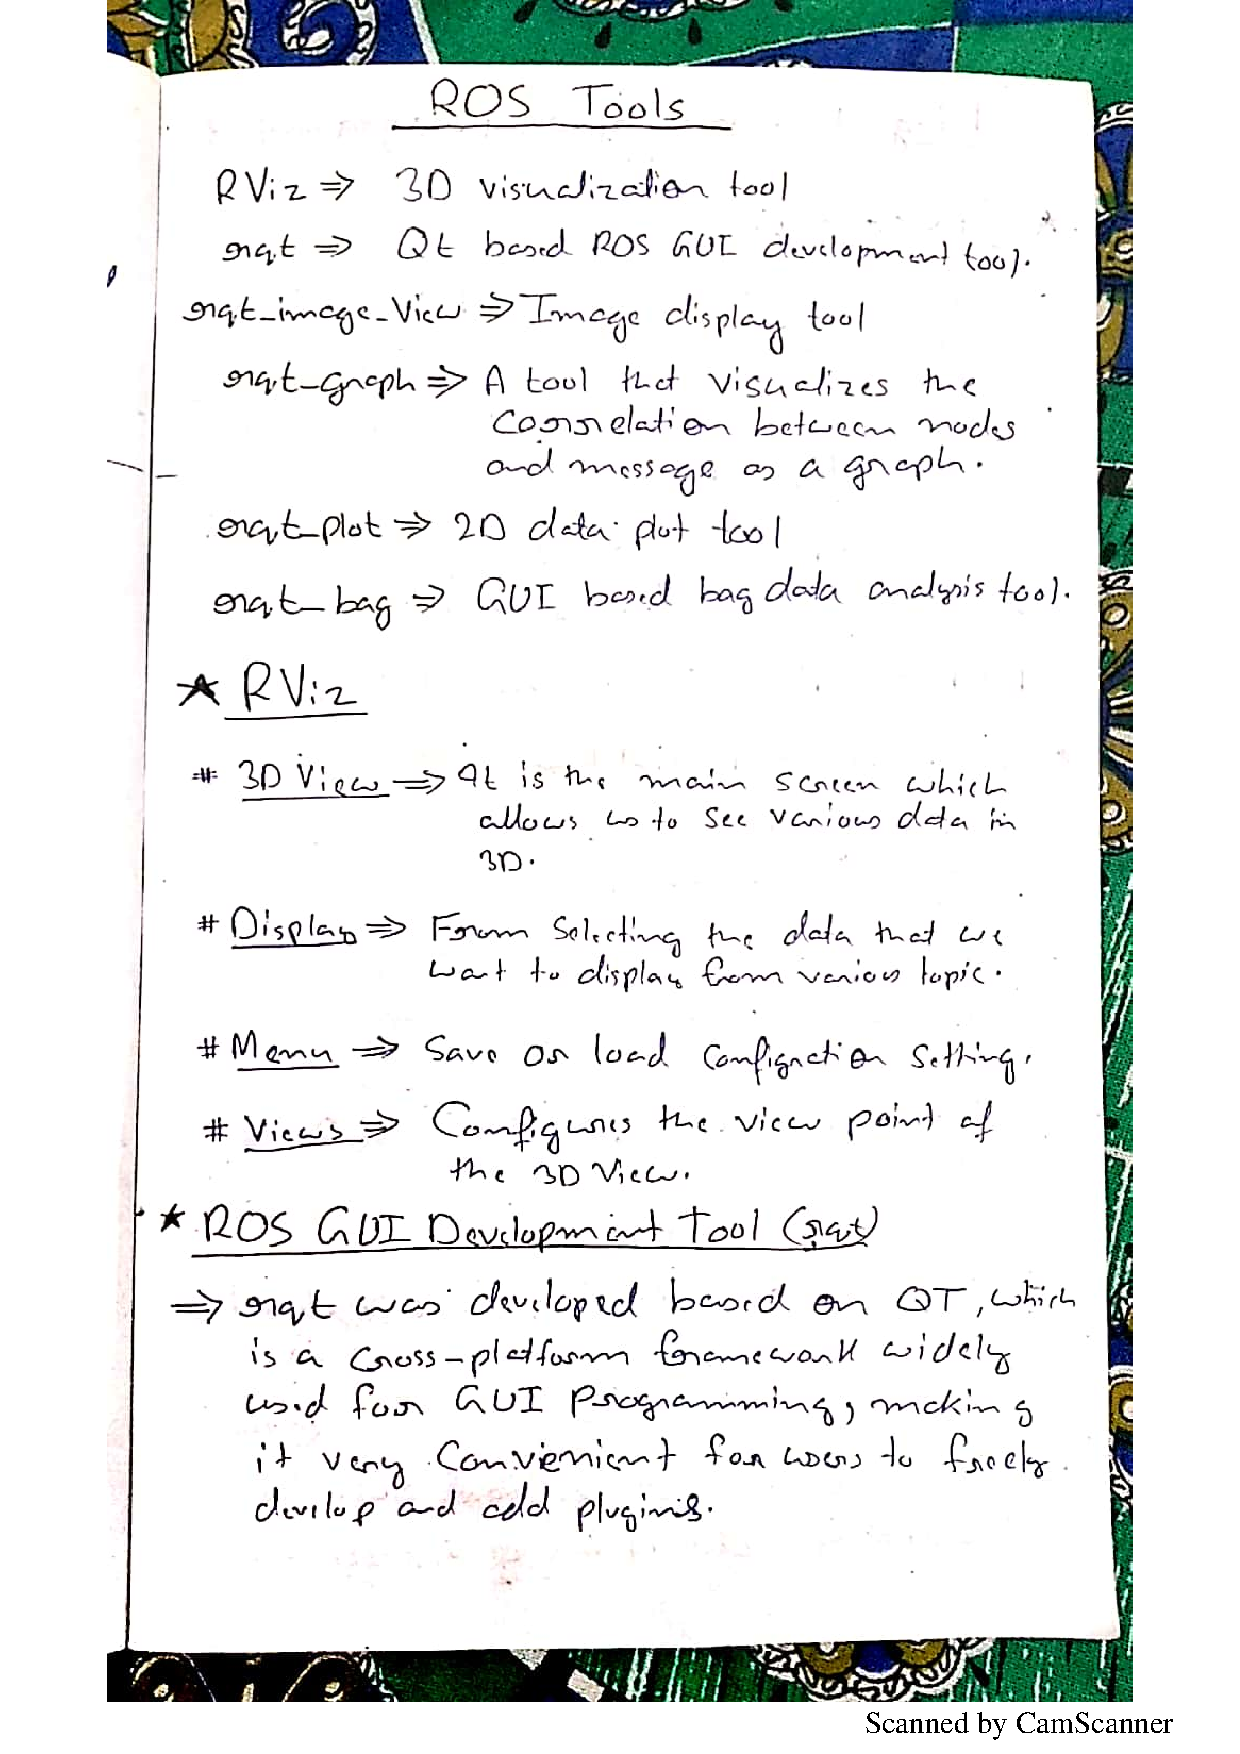
\includepdf[page=-]{./raw_files/11.pdf}

\chapter{Things to know before programming ROS}
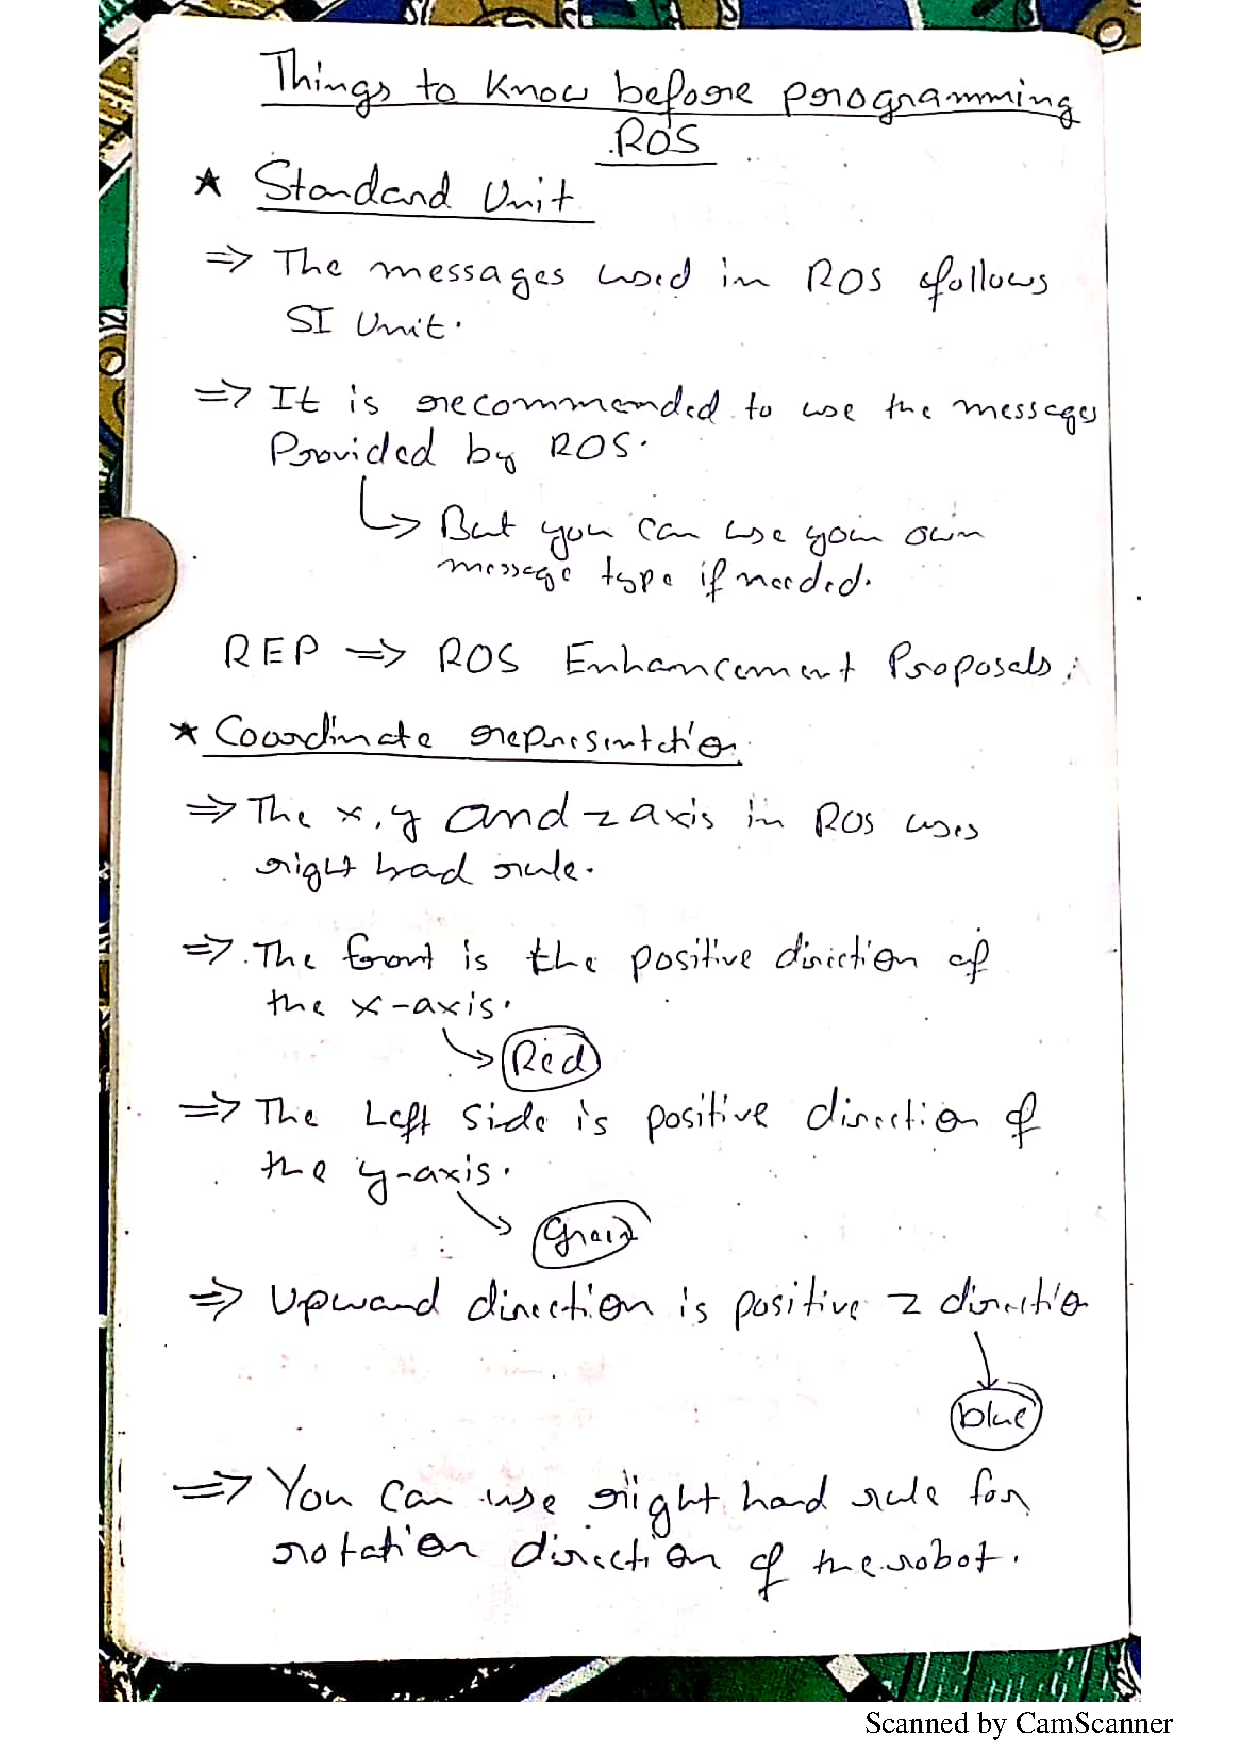
\includepdf[page=-]{./raw_files/12.pdf}

\chapter{Robot Sensor Motor}
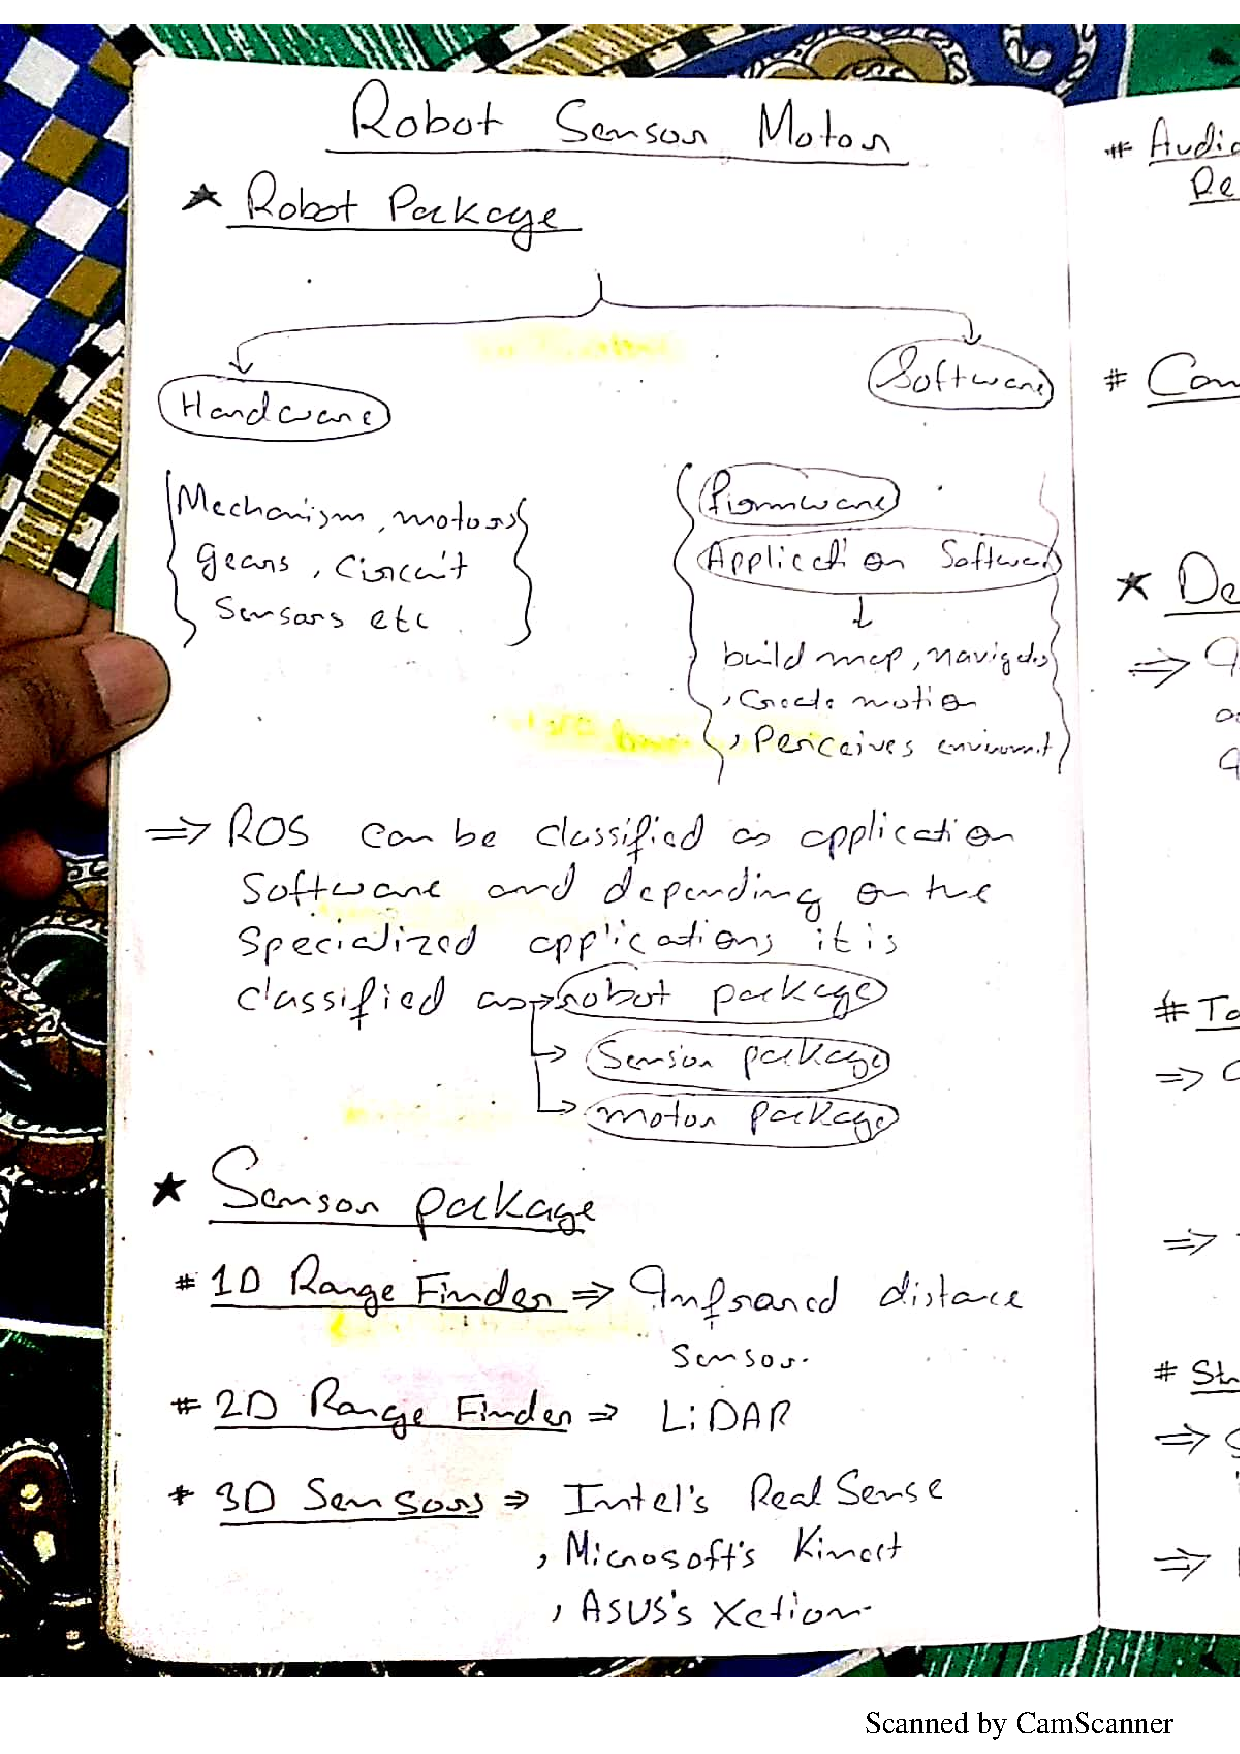
\includepdf[page=-]{./raw_files/13.pdf}

\chapter{SLAM Theory}
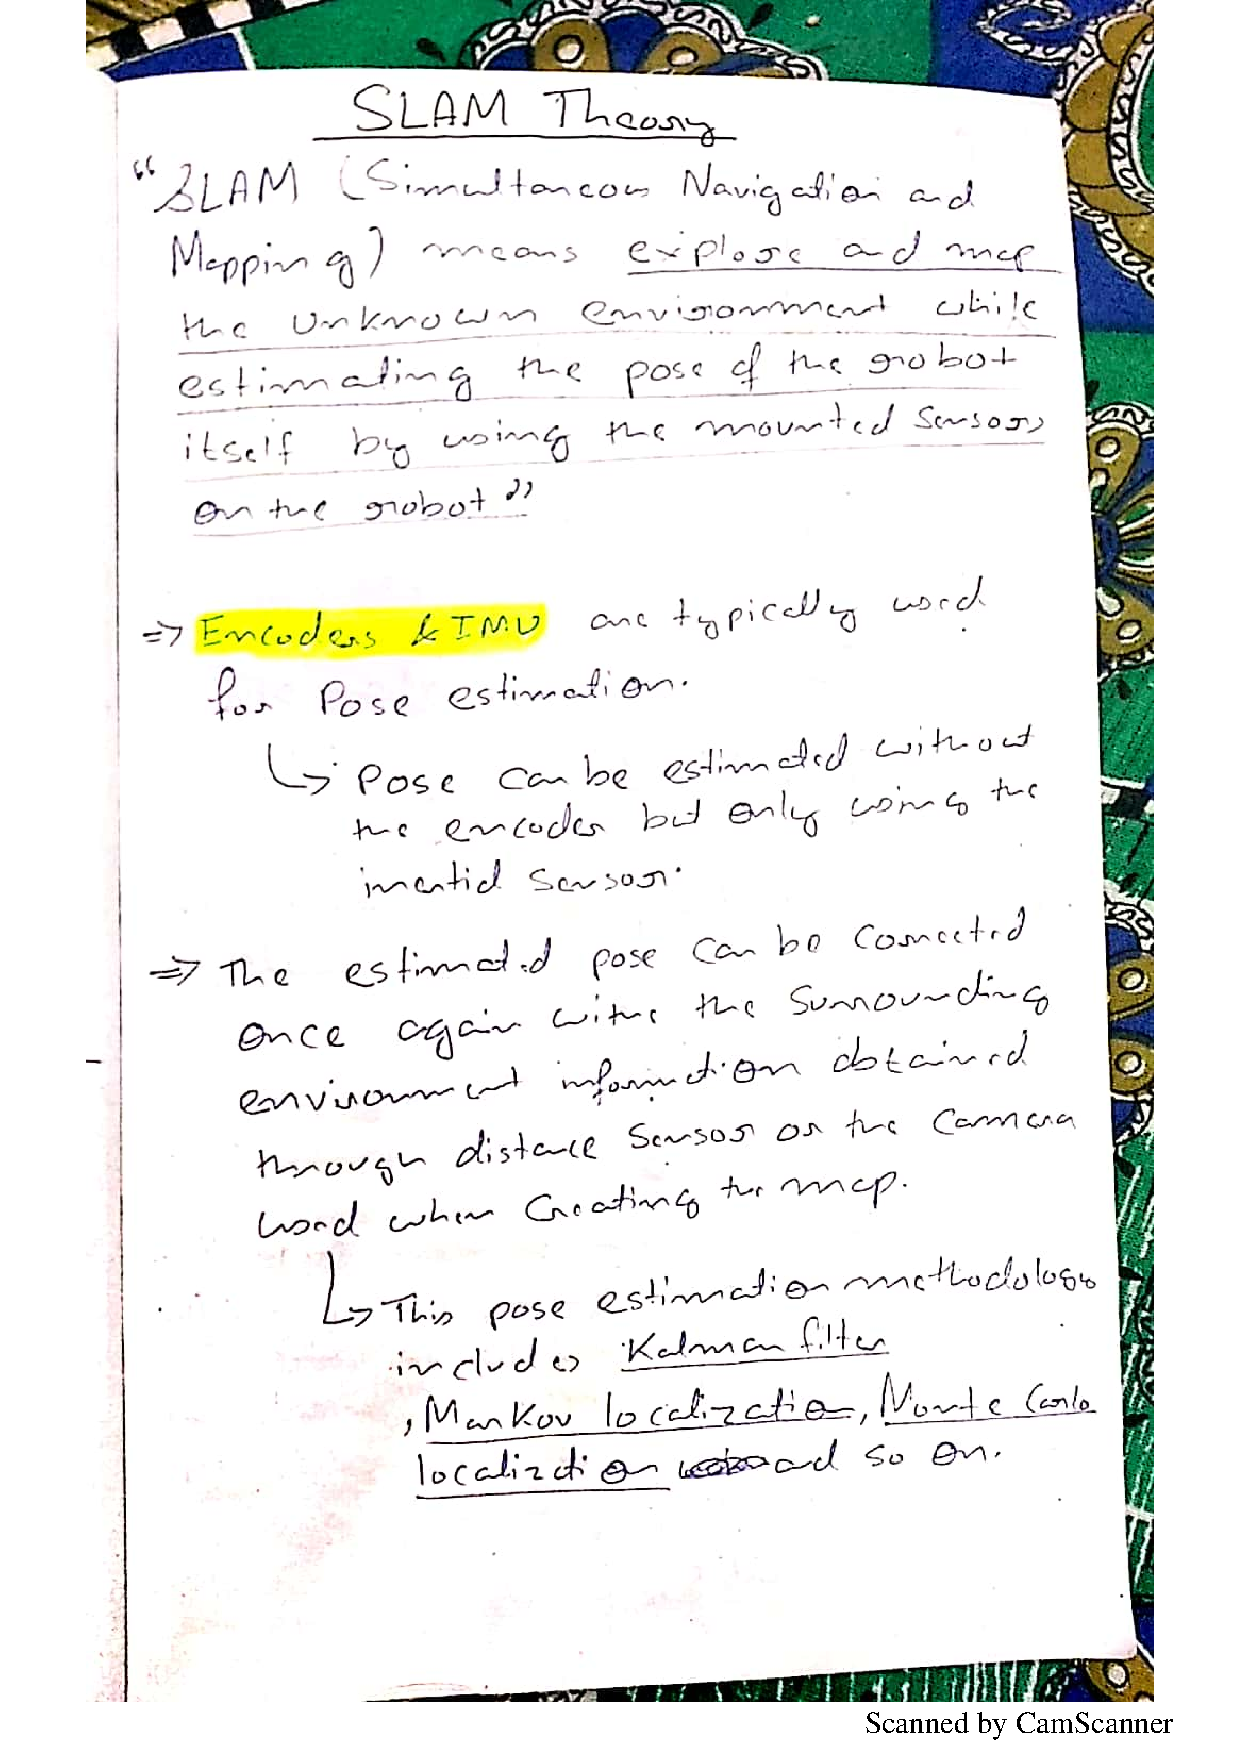
\includepdf[page=-]{./raw_files/14.pdf}

\chapter{Navigation Theory}
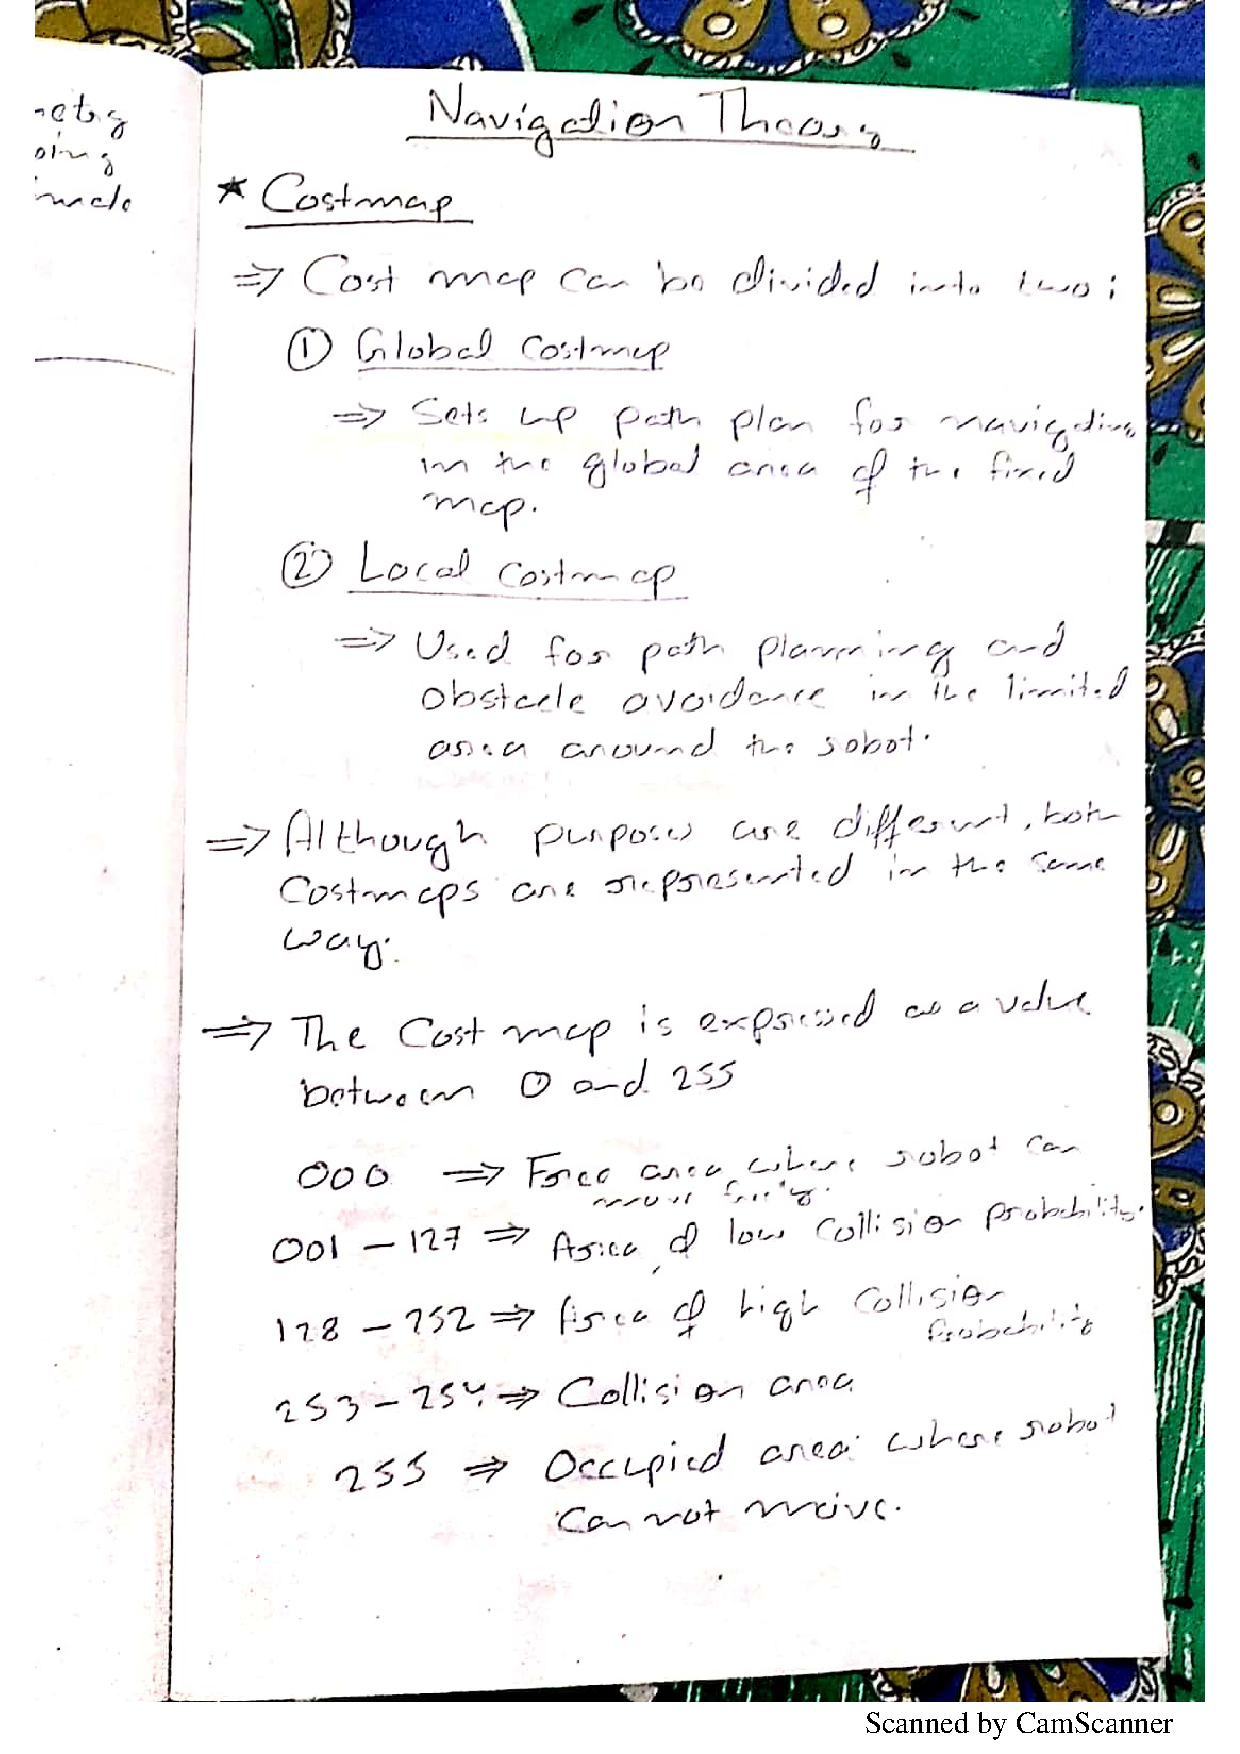
\includepdf[page=-]{./raw_files/15.pdf}

\chapter{Ros Developers Guide}
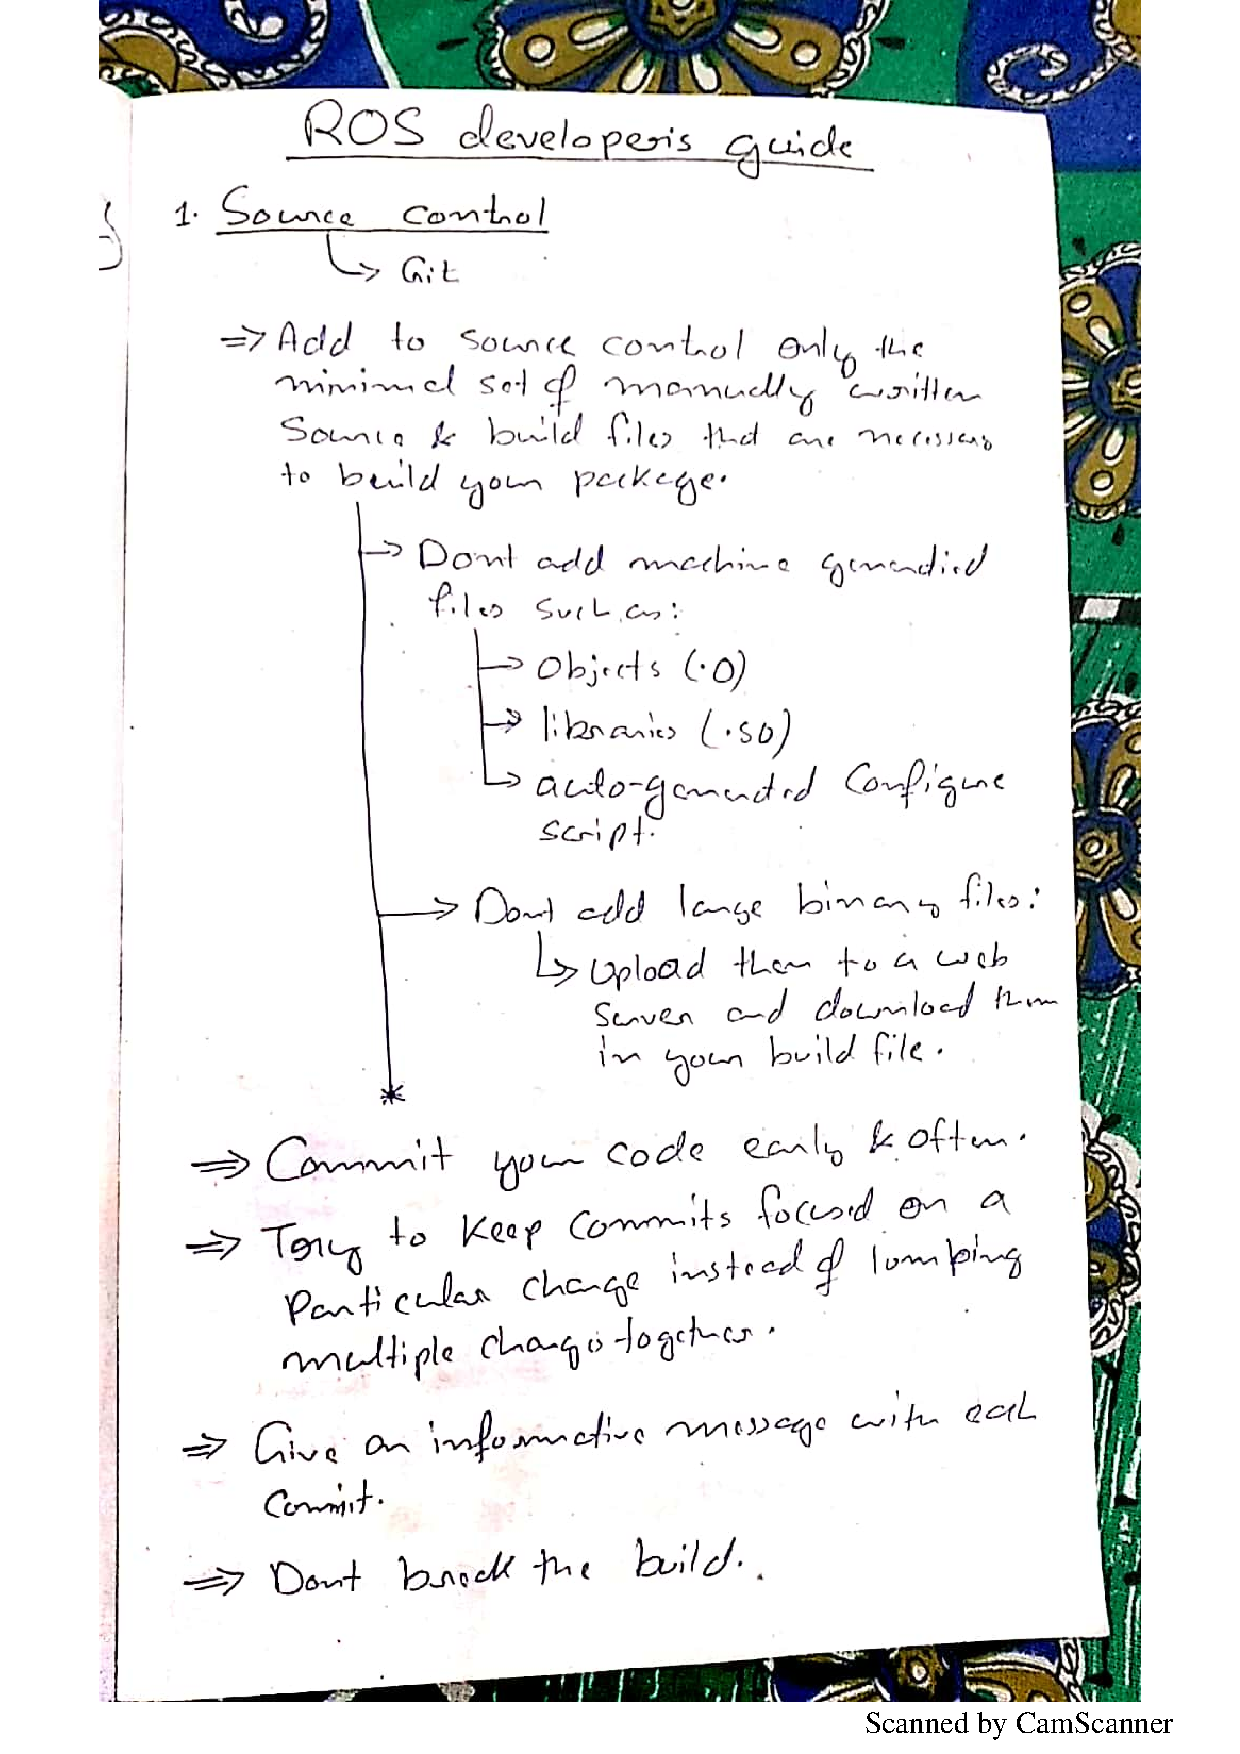
\includepdf[page=-]{./raw_files/16.pdf}

\chapter{package.xml}
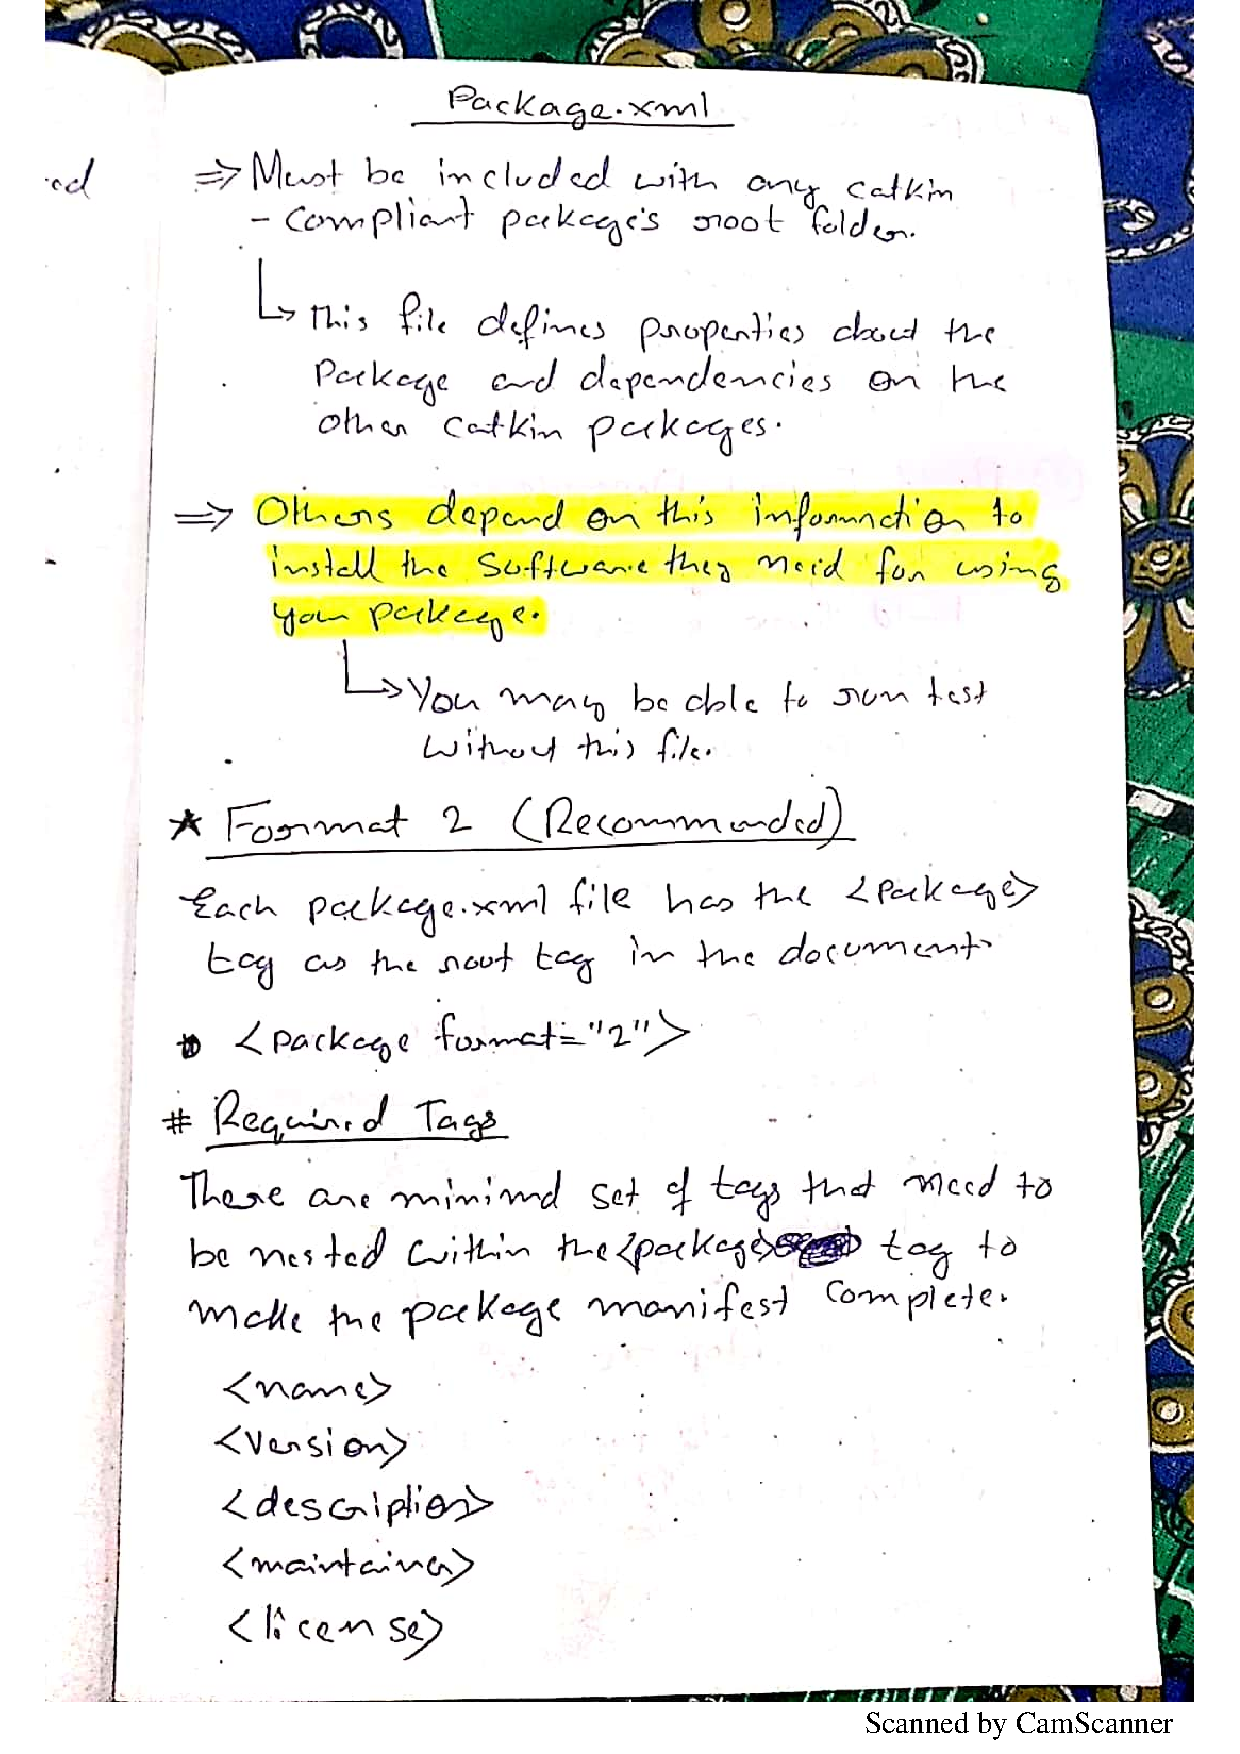
\includepdf[page=-]{./raw_files/17.pdf}

\chapter{CMakeList.txt}
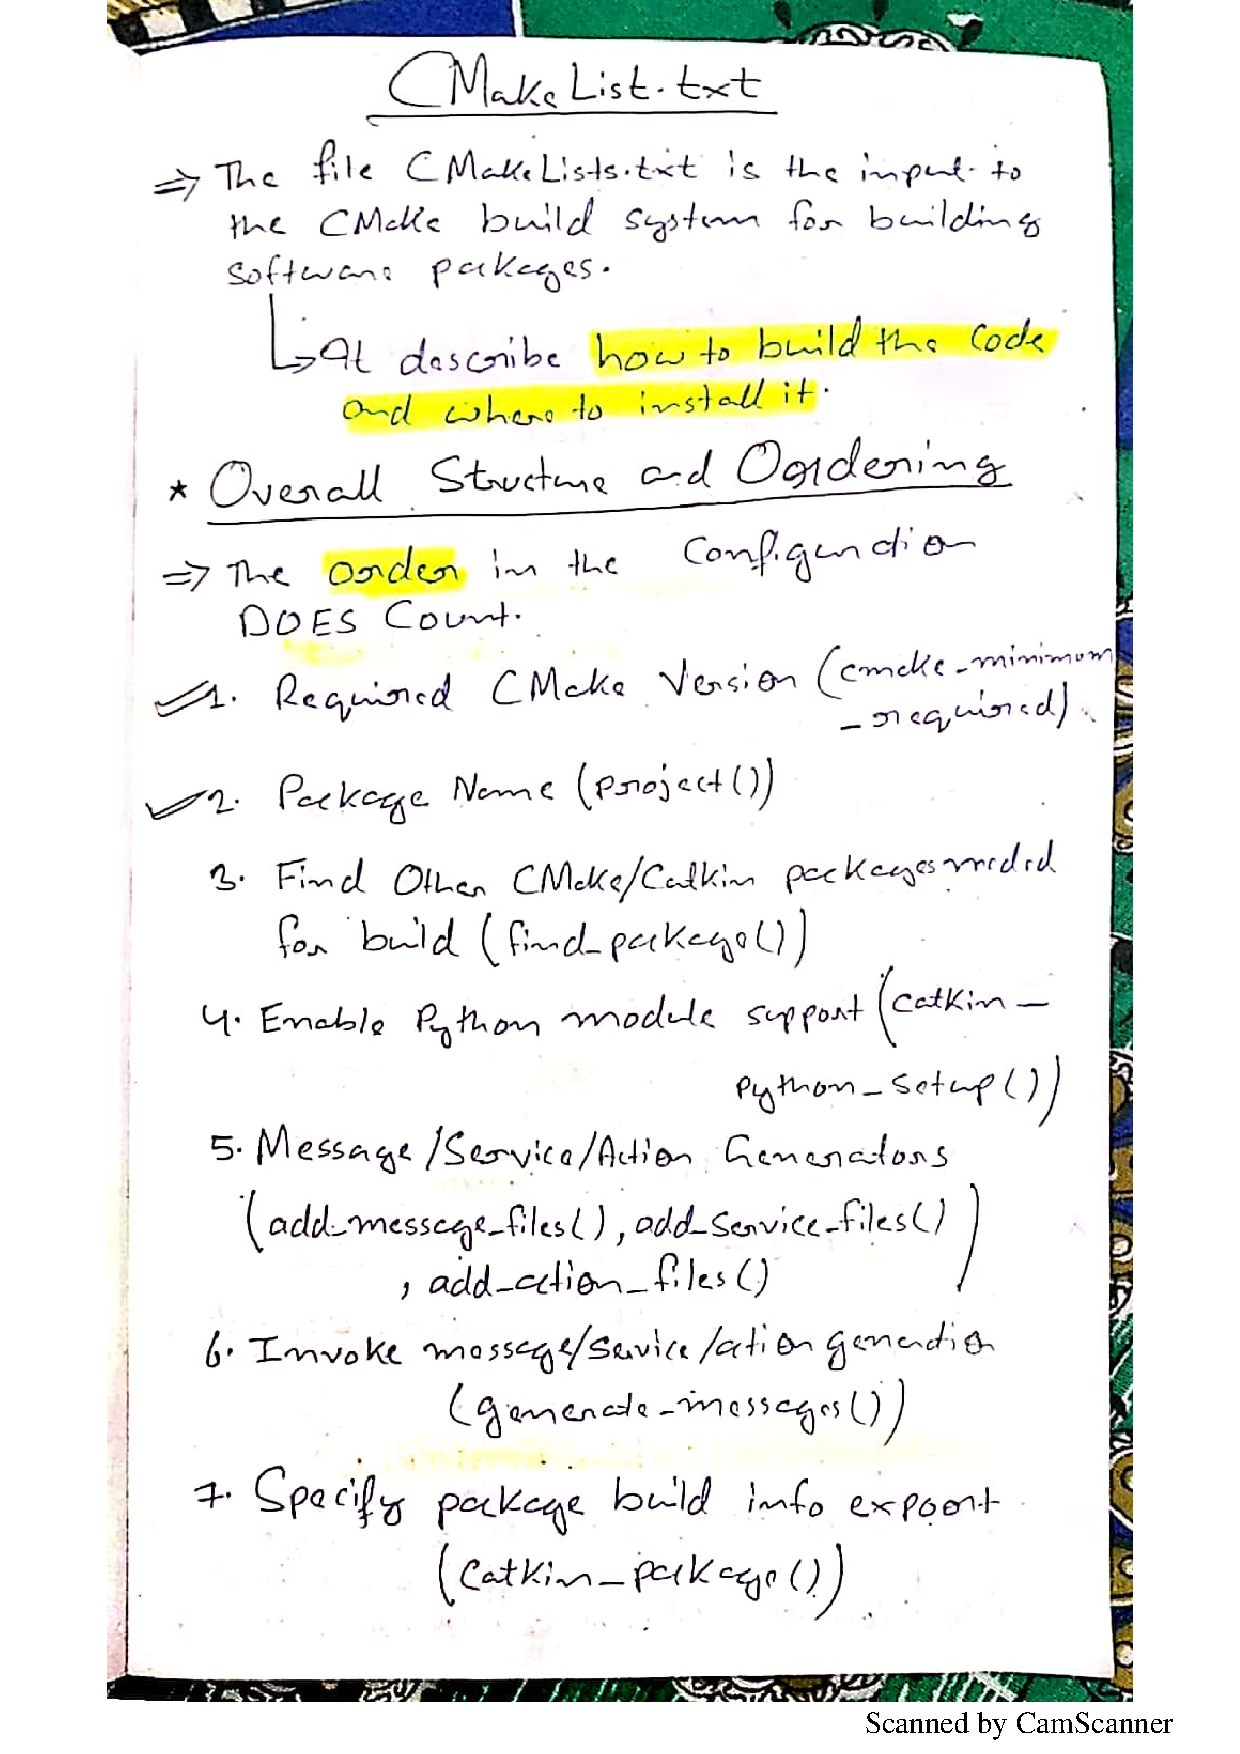
\includepdf[page=-]{./raw_files/18.pdf}

\chapter{Doxygen}
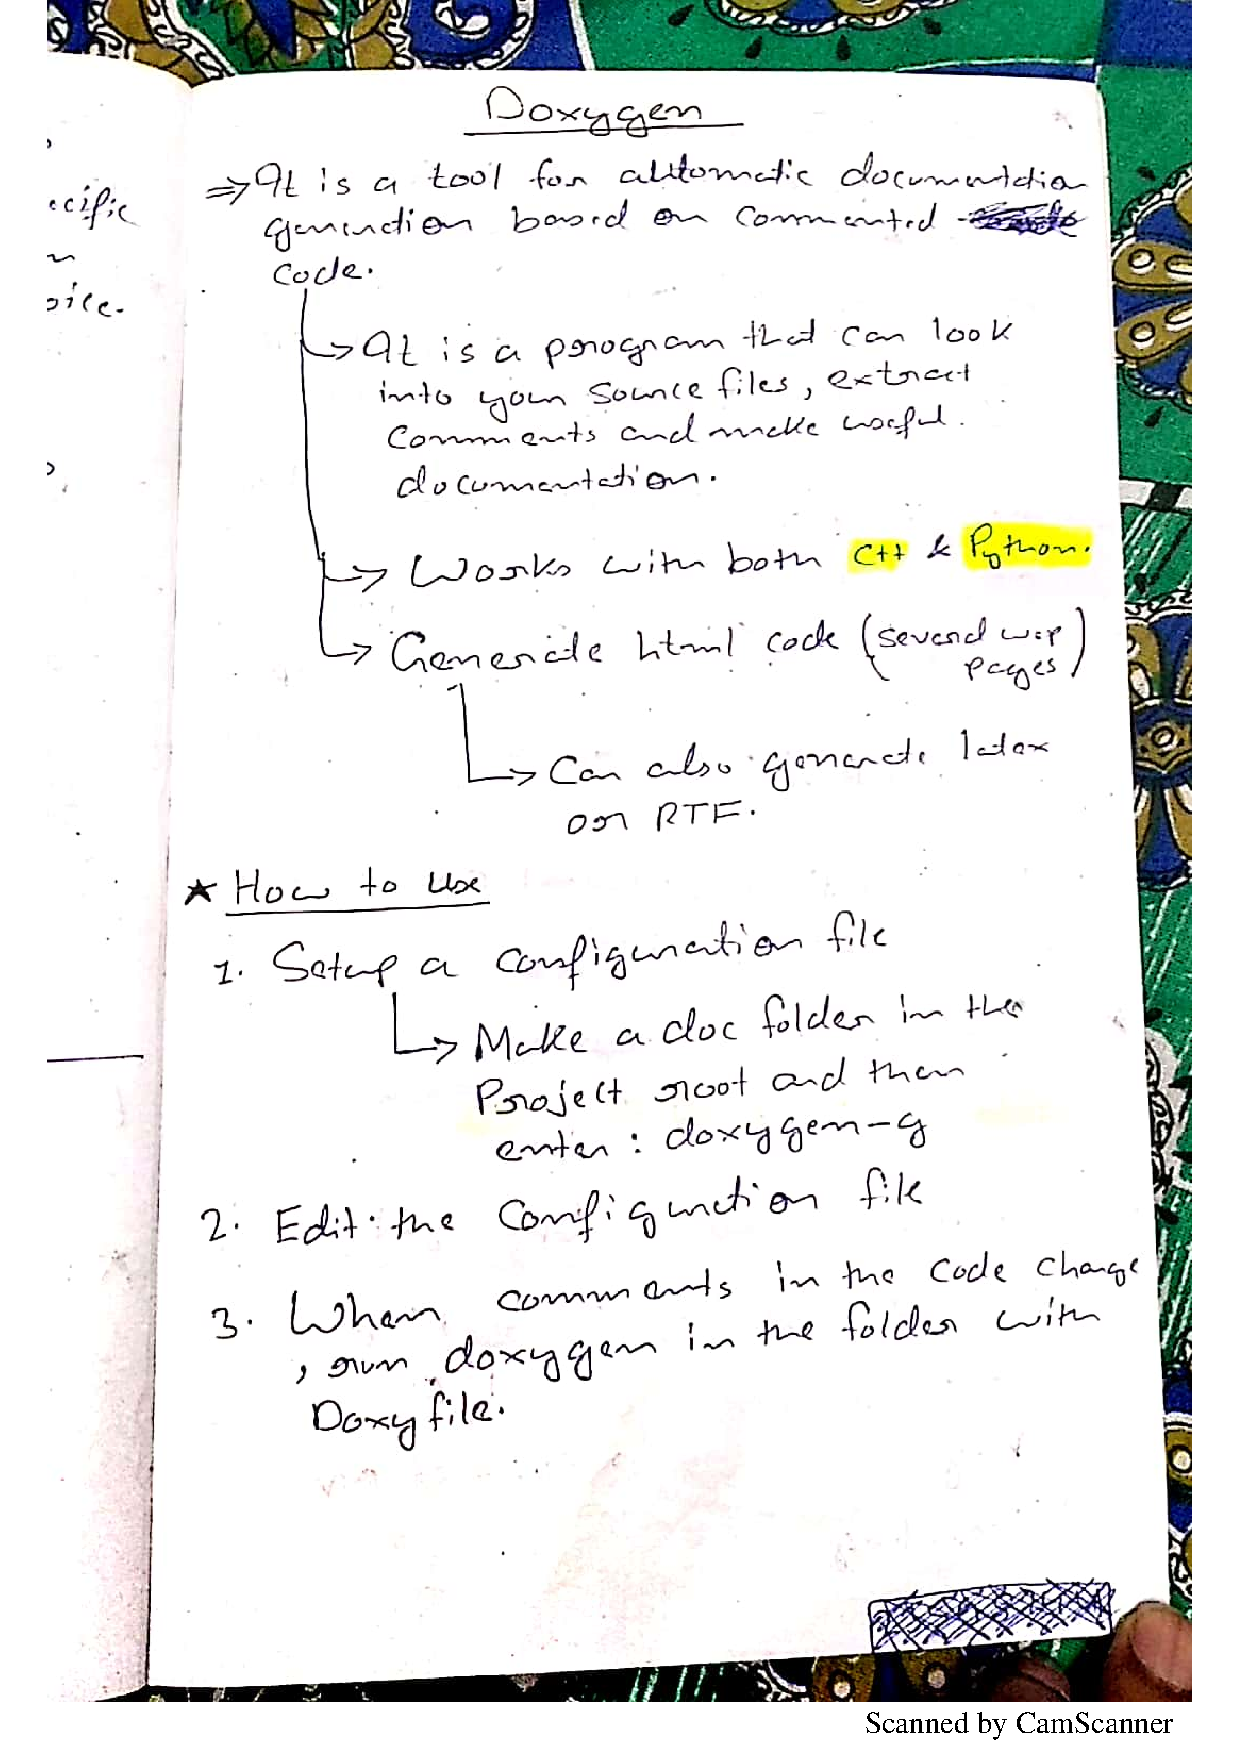
\includepdf[page=-]{./raw_files/19.pdf}

\chapter{Working with Pluginlib, Nodelets and Gazebo Plugins}
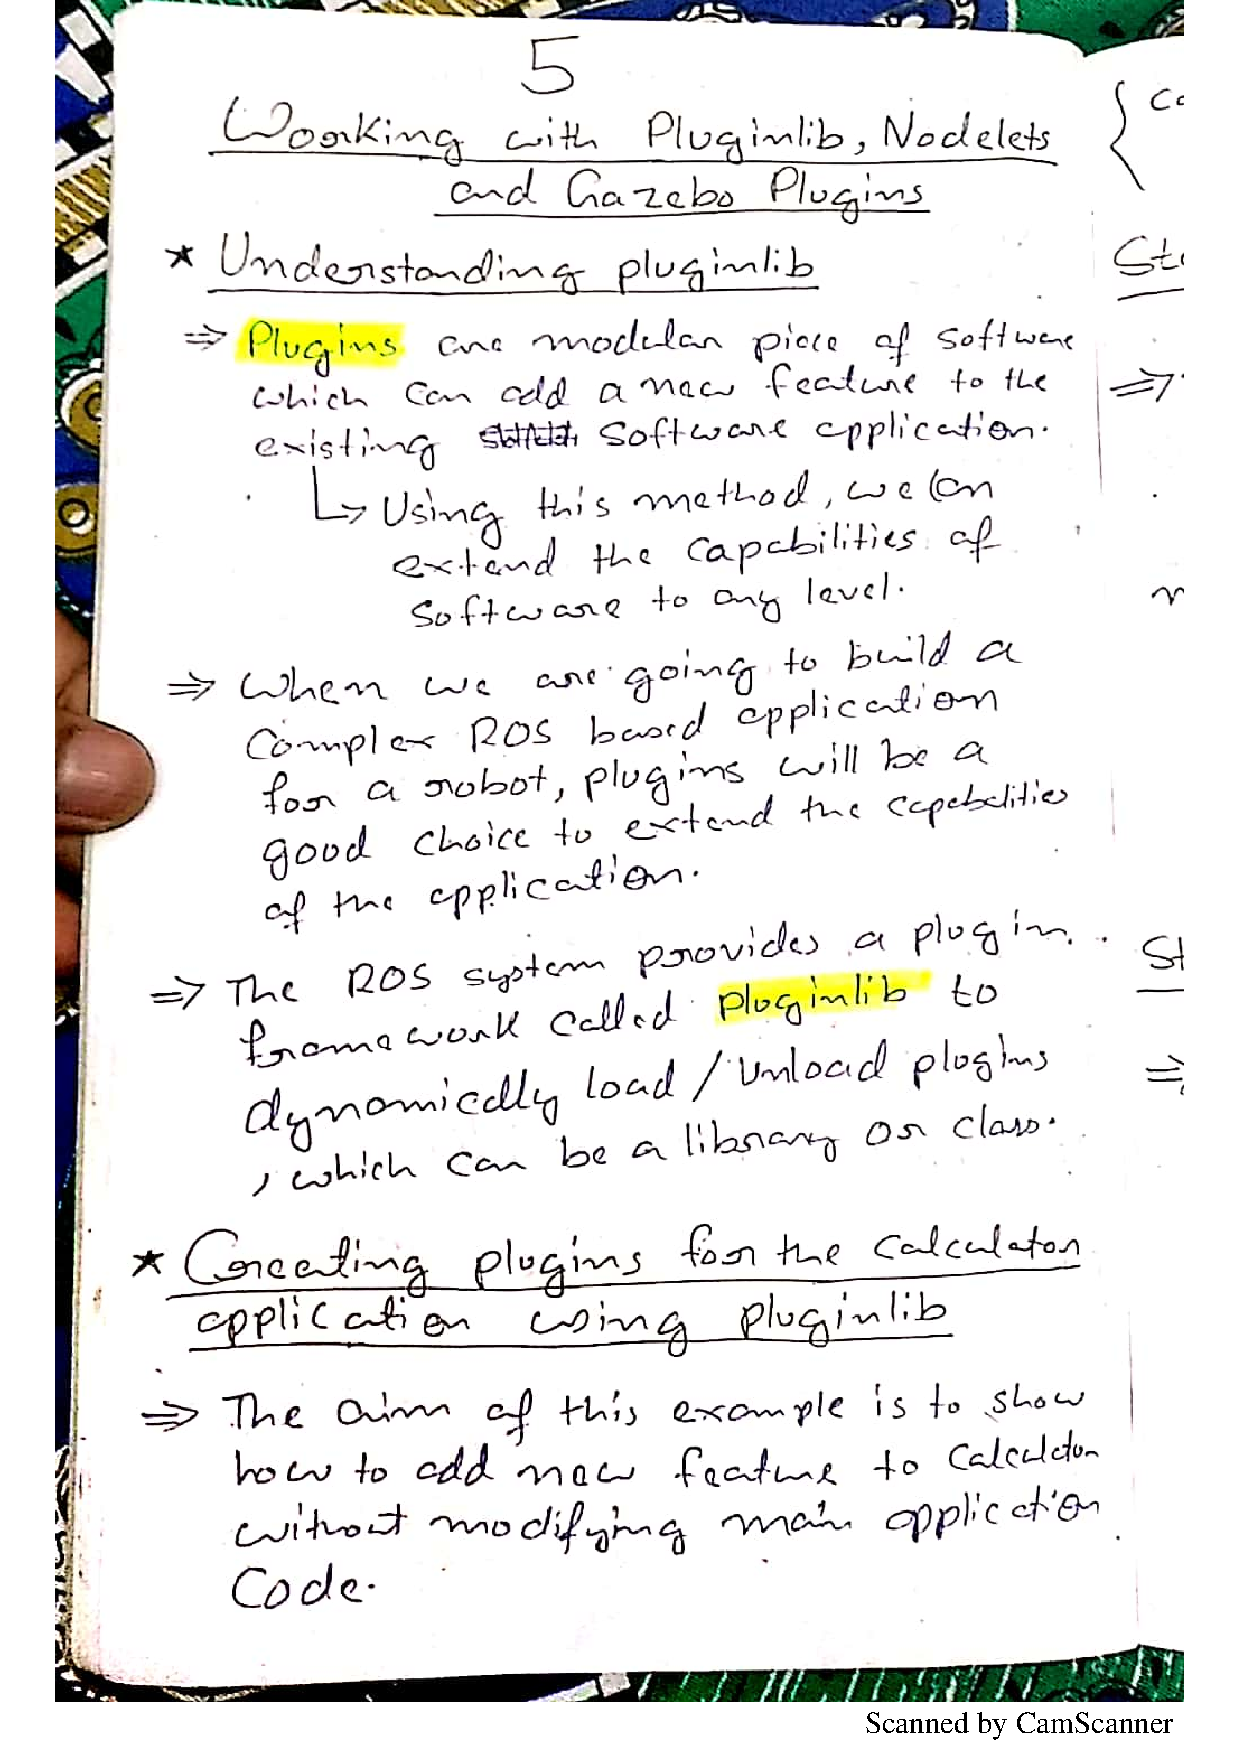
\includepdf[page=-]{./raw_files/20.pdf}

\chapter{Writing ROS Controllers and Visulization Plugins}
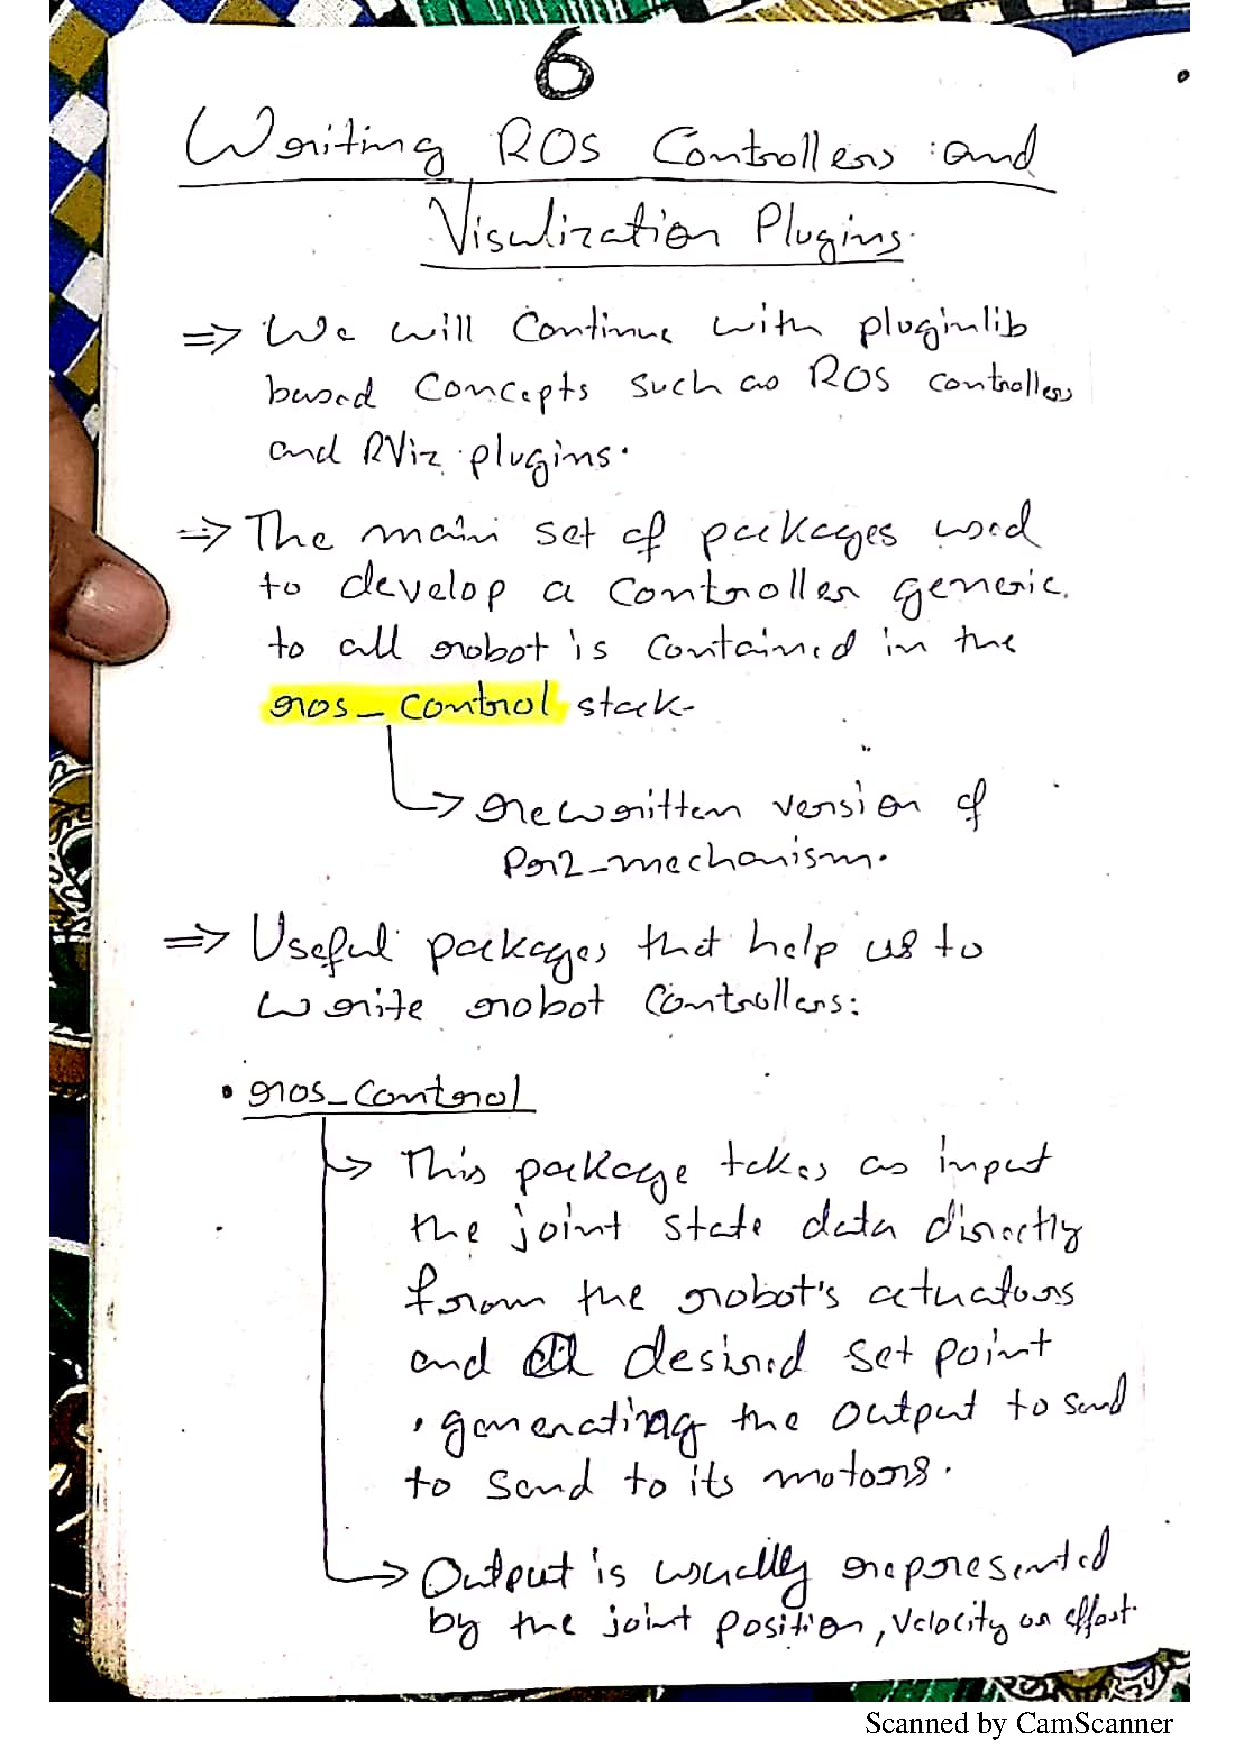
\includepdf[page=-]{./raw_files/21.pdf}

\chapter{Working with ROS actionlib}
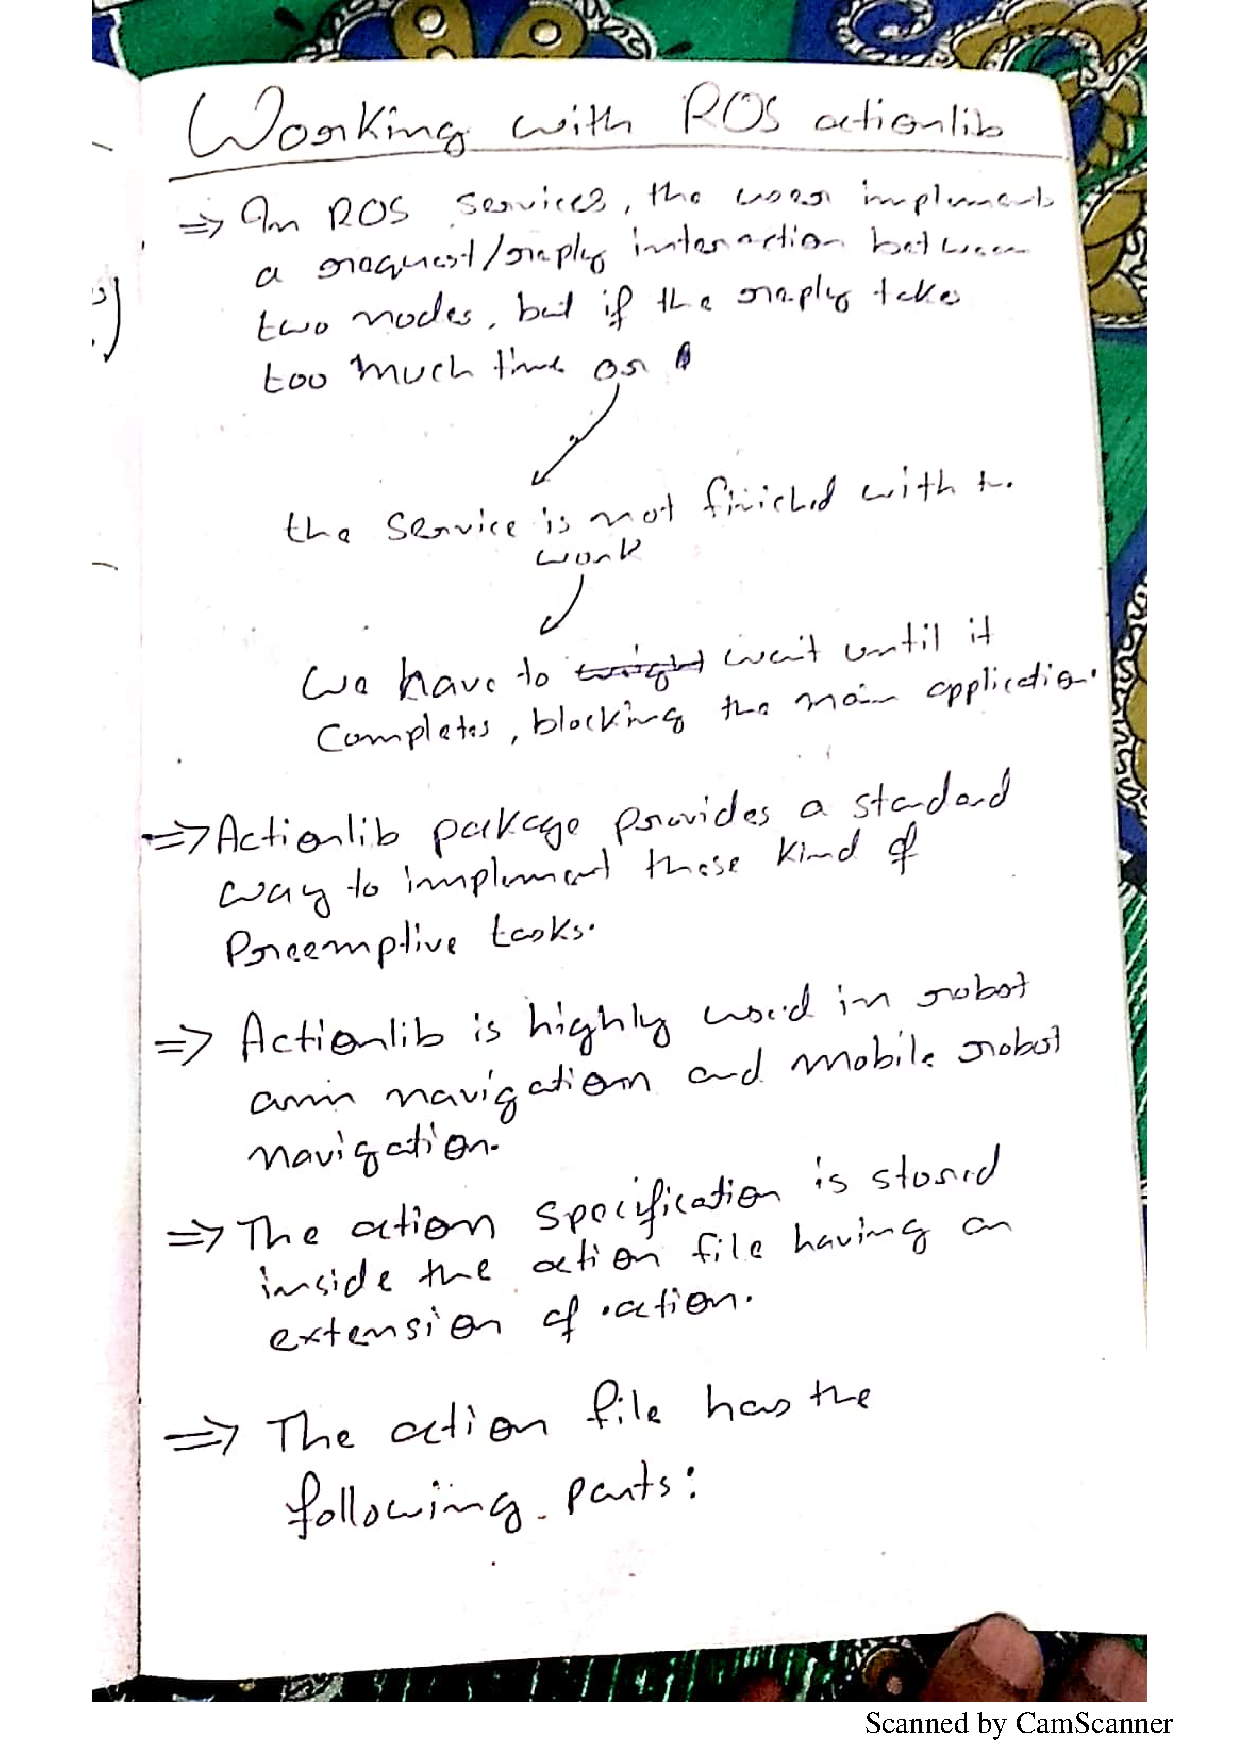
\includepdf[page=-]{./raw_files/22.pdf}

\chapter{Applications of topic, service and actionlib}
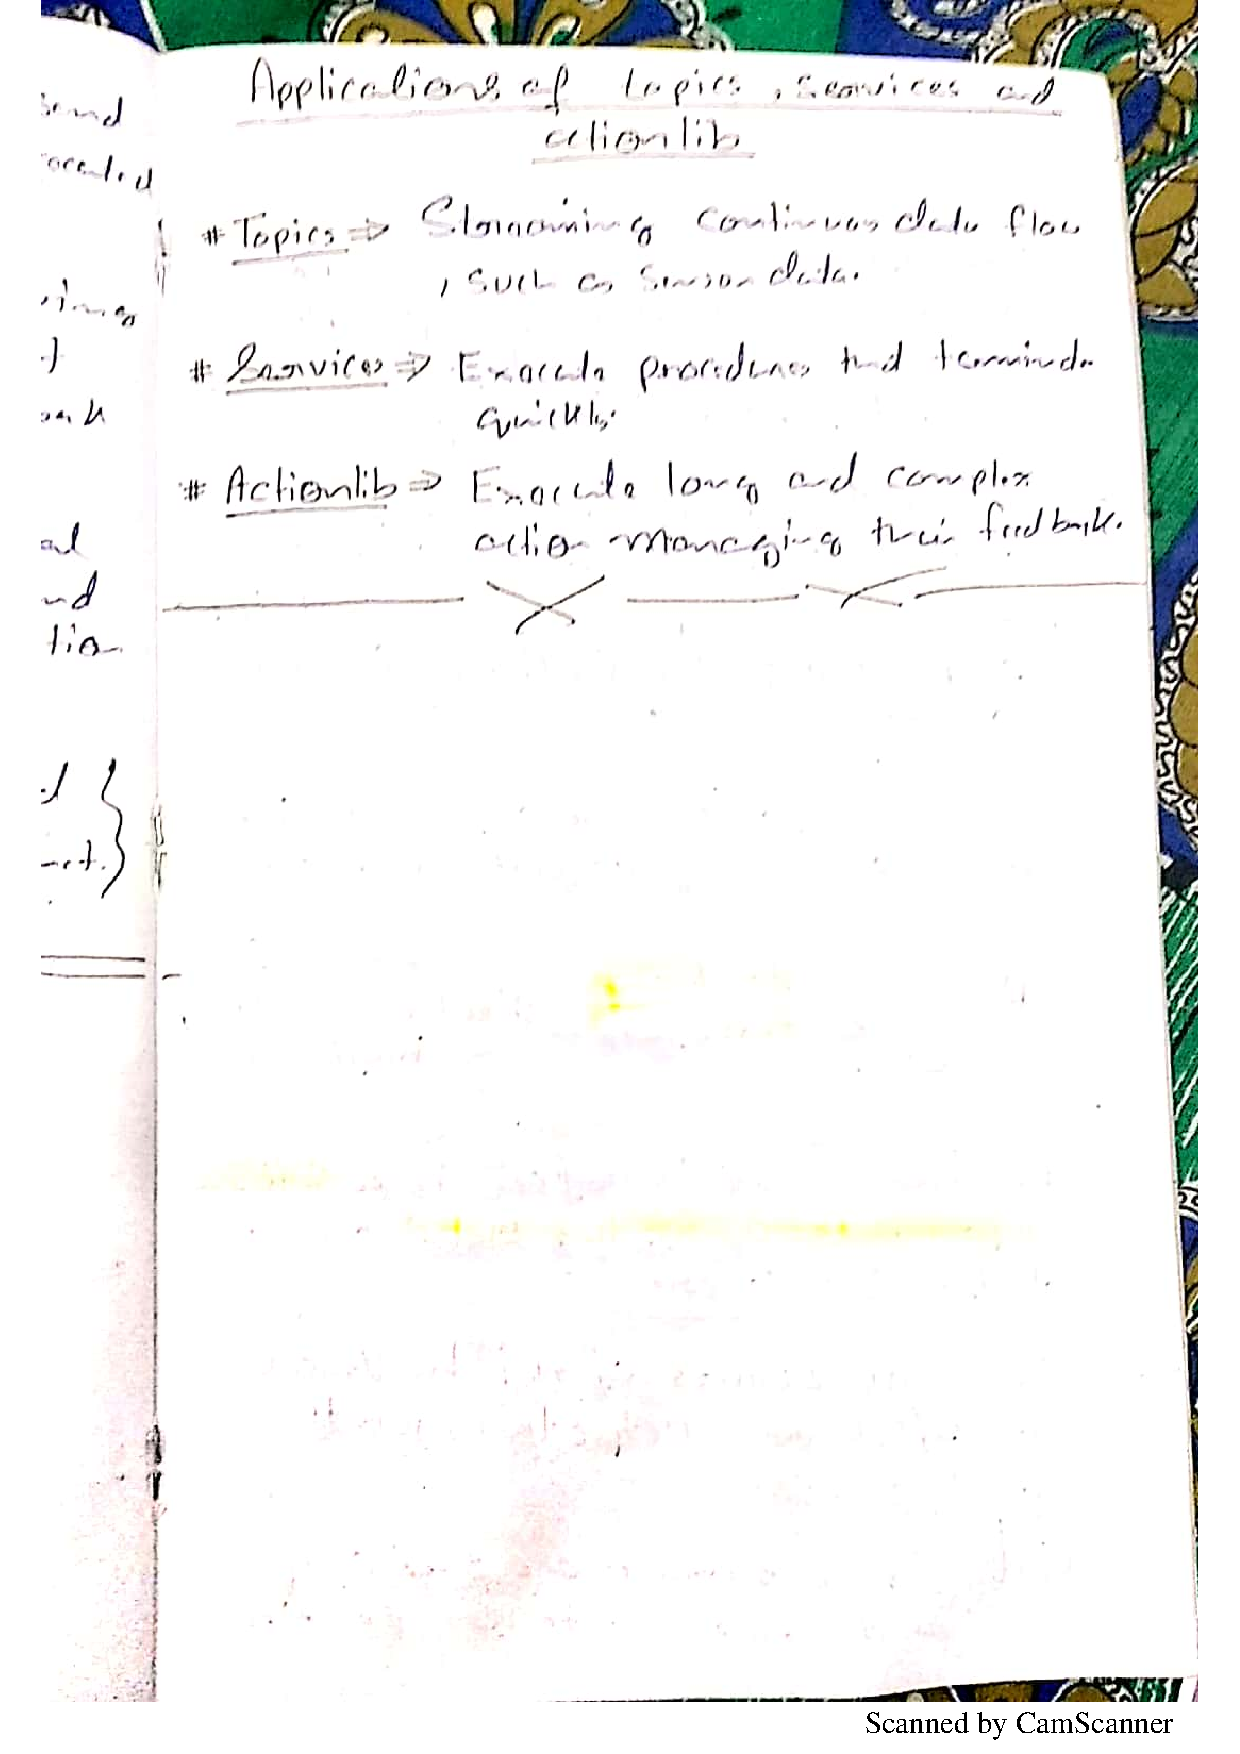
\includepdf[page=-]{./raw_files/23.pdf}

\chapter{Moving Robot Joints Using ROS Controllers in Gazebo}
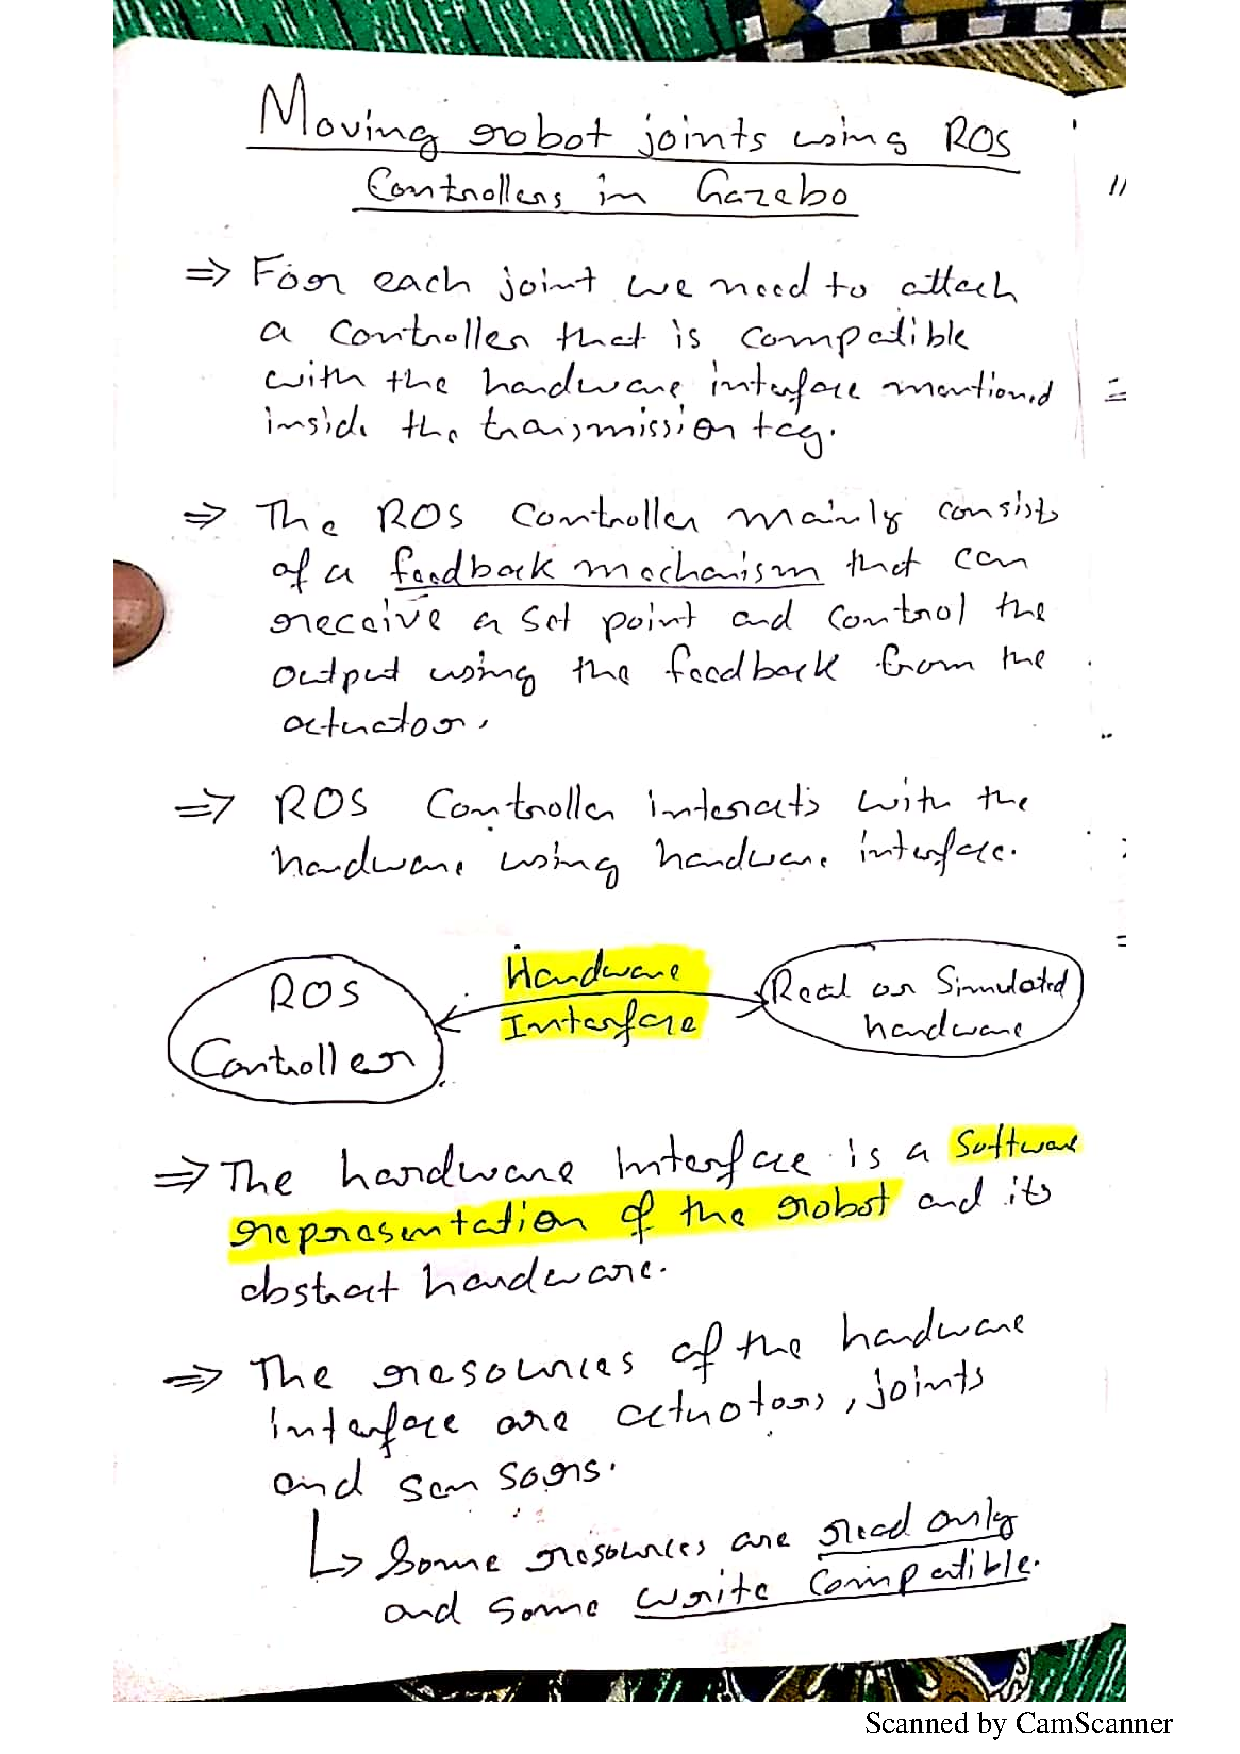
\includepdf[page=-]{./raw_files/24.pdf}

\chapter{Working with a robot in Simulation}
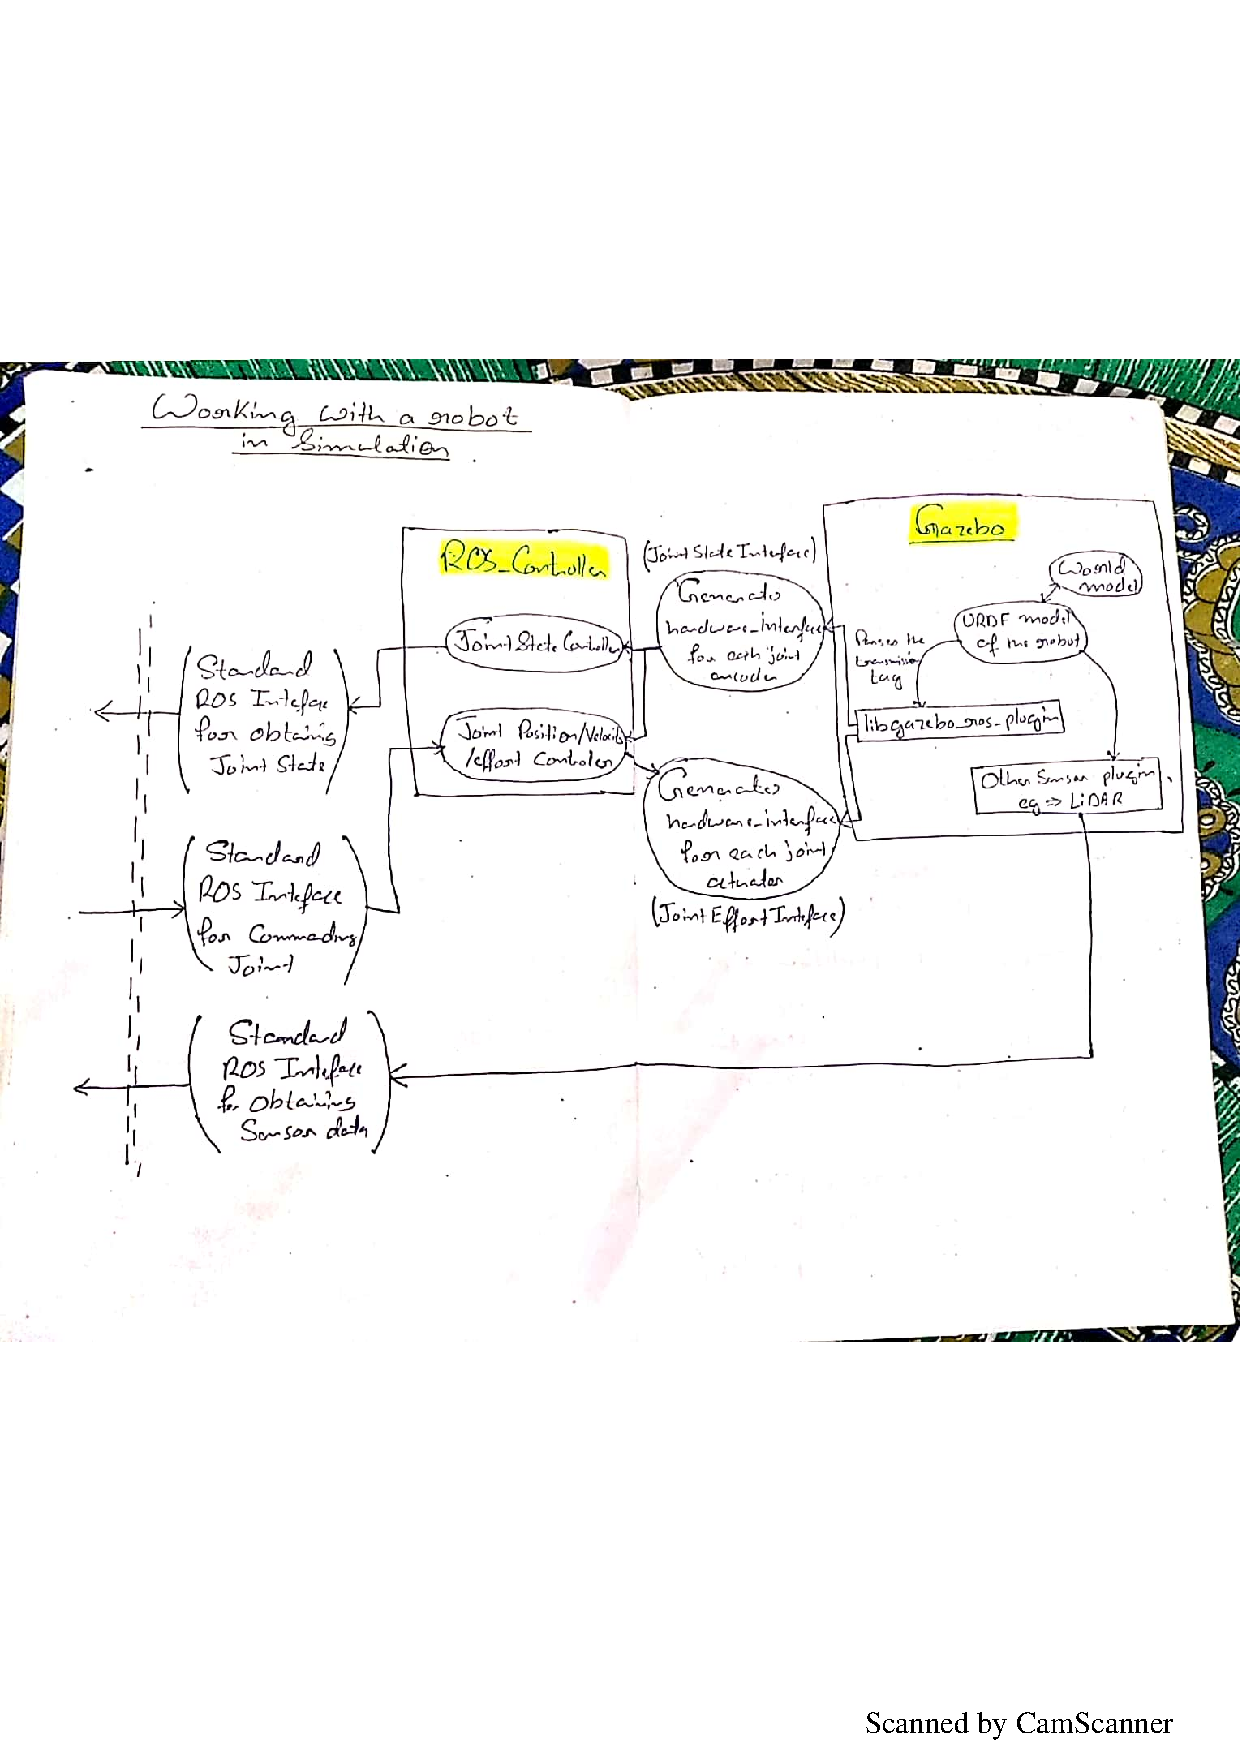
\includepdf[page=-]{./raw_files/25.pdf}

\chapter{Working with real Robot}
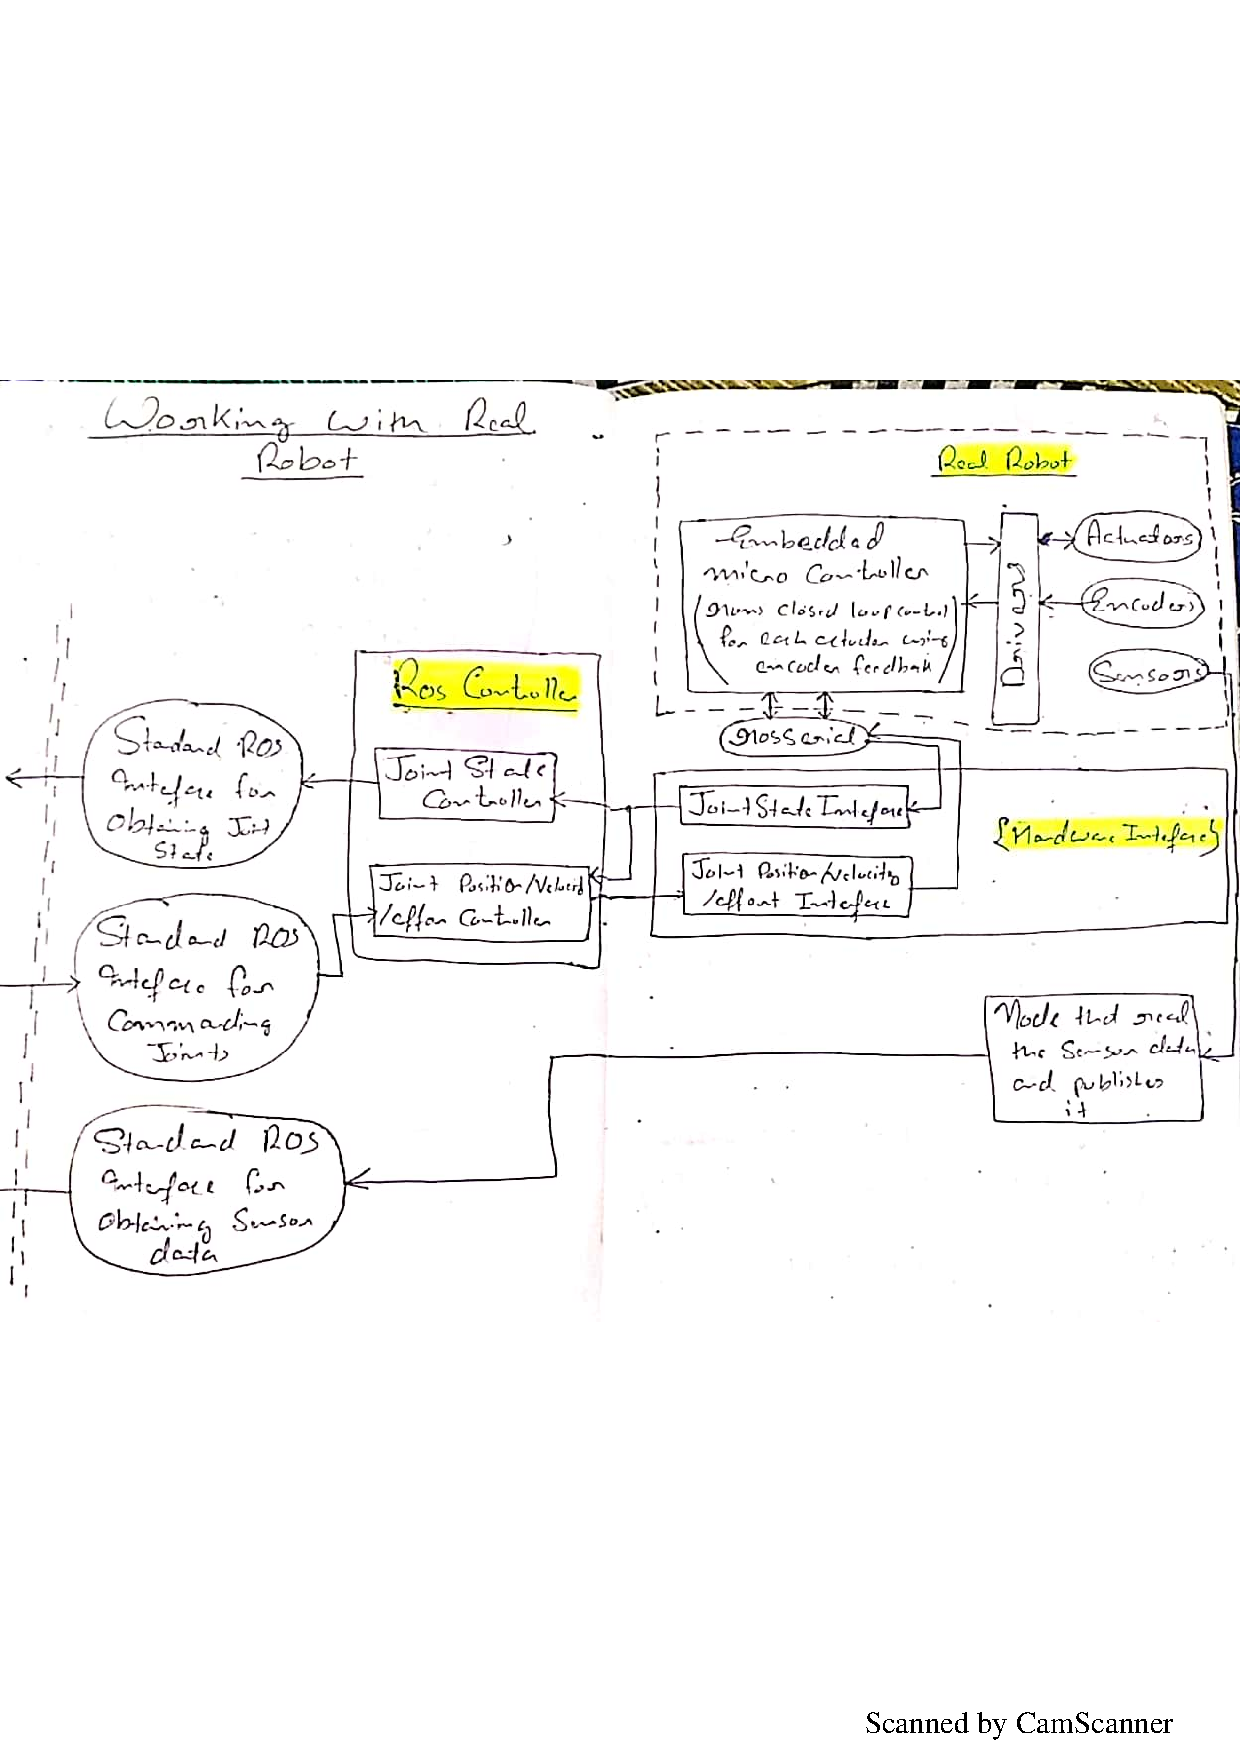
\includepdf[page=-]{./raw_files/26.pdf}

\chapter{Robot State Publisher}
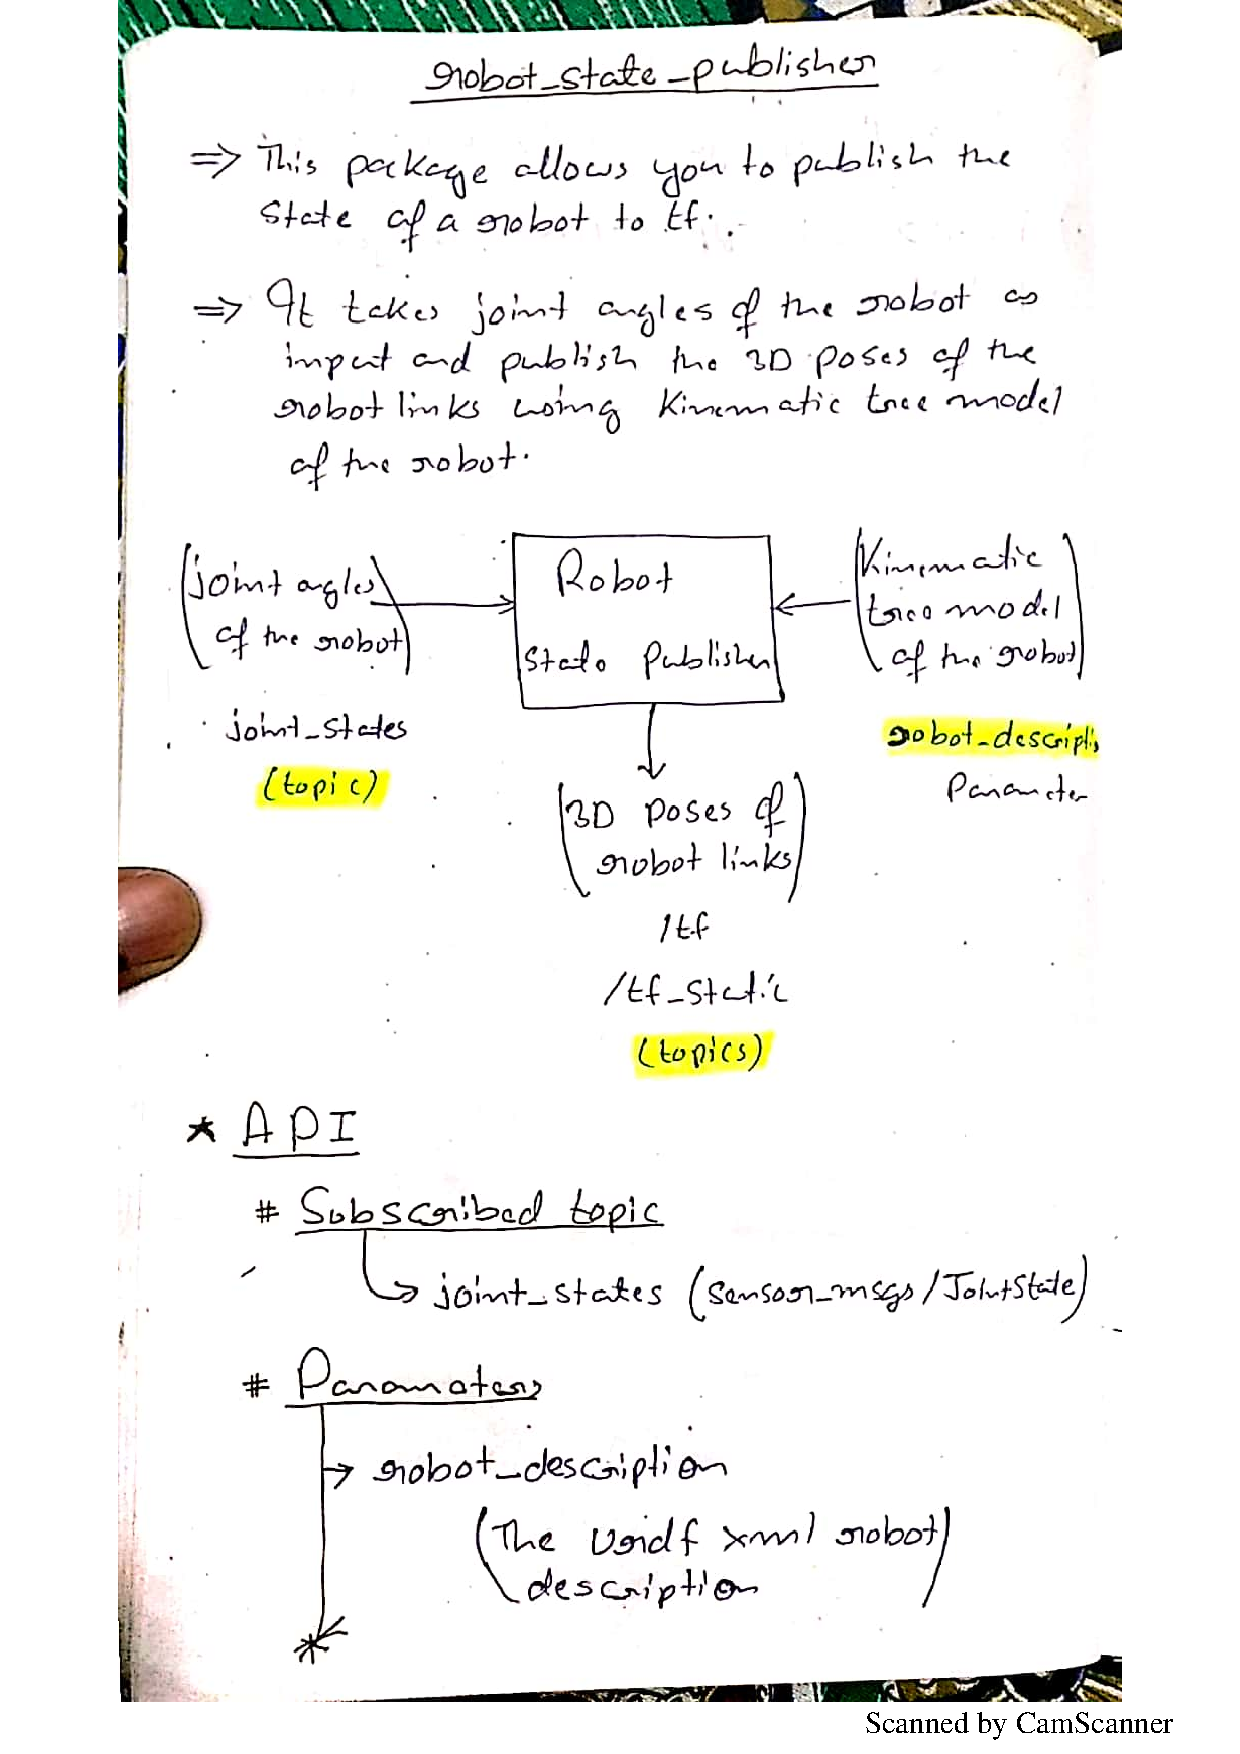
\includepdf[page=-]{./raw_files/27.pdf}

\chapter{Navigation Tutorial}
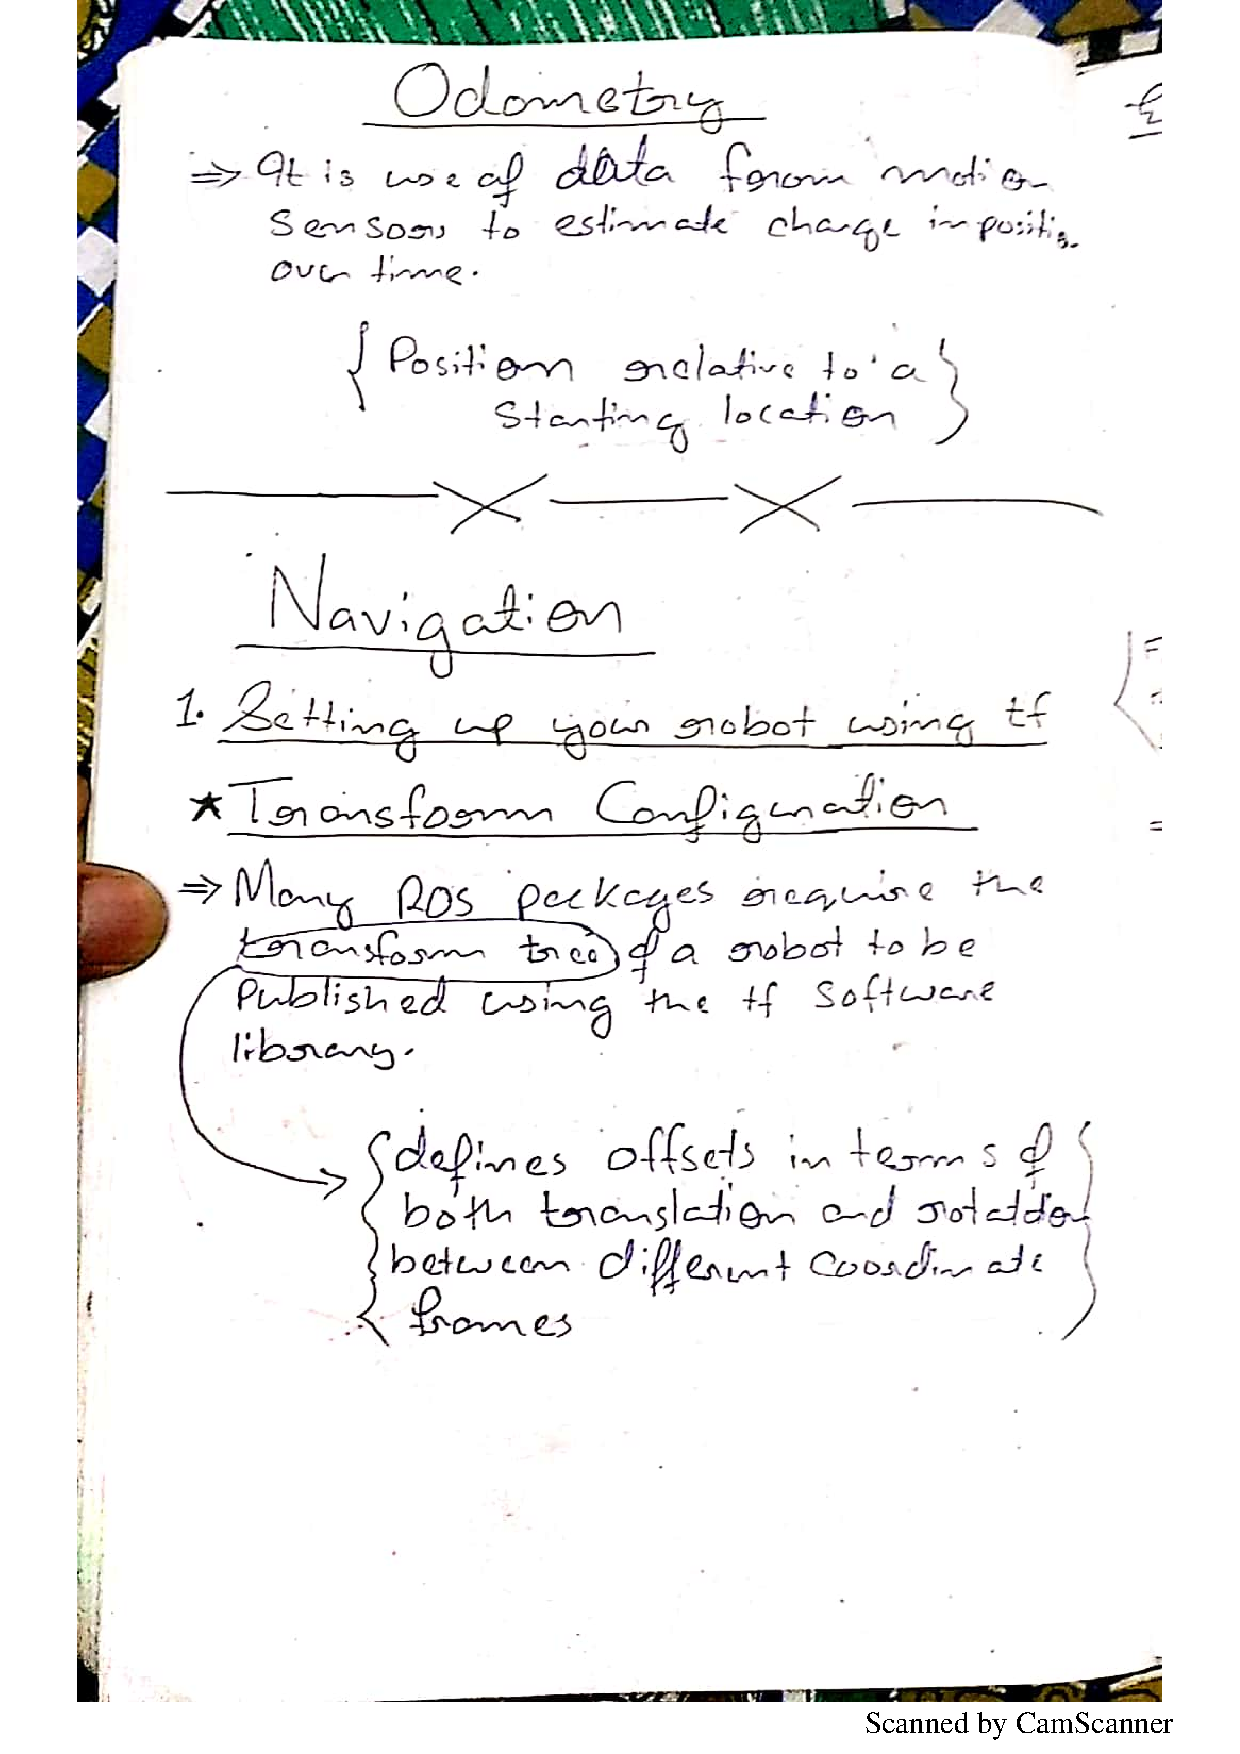
\includepdf[page=-]{./raw_files/28.pdf}

\chapter{Running ROS across multiple machine}
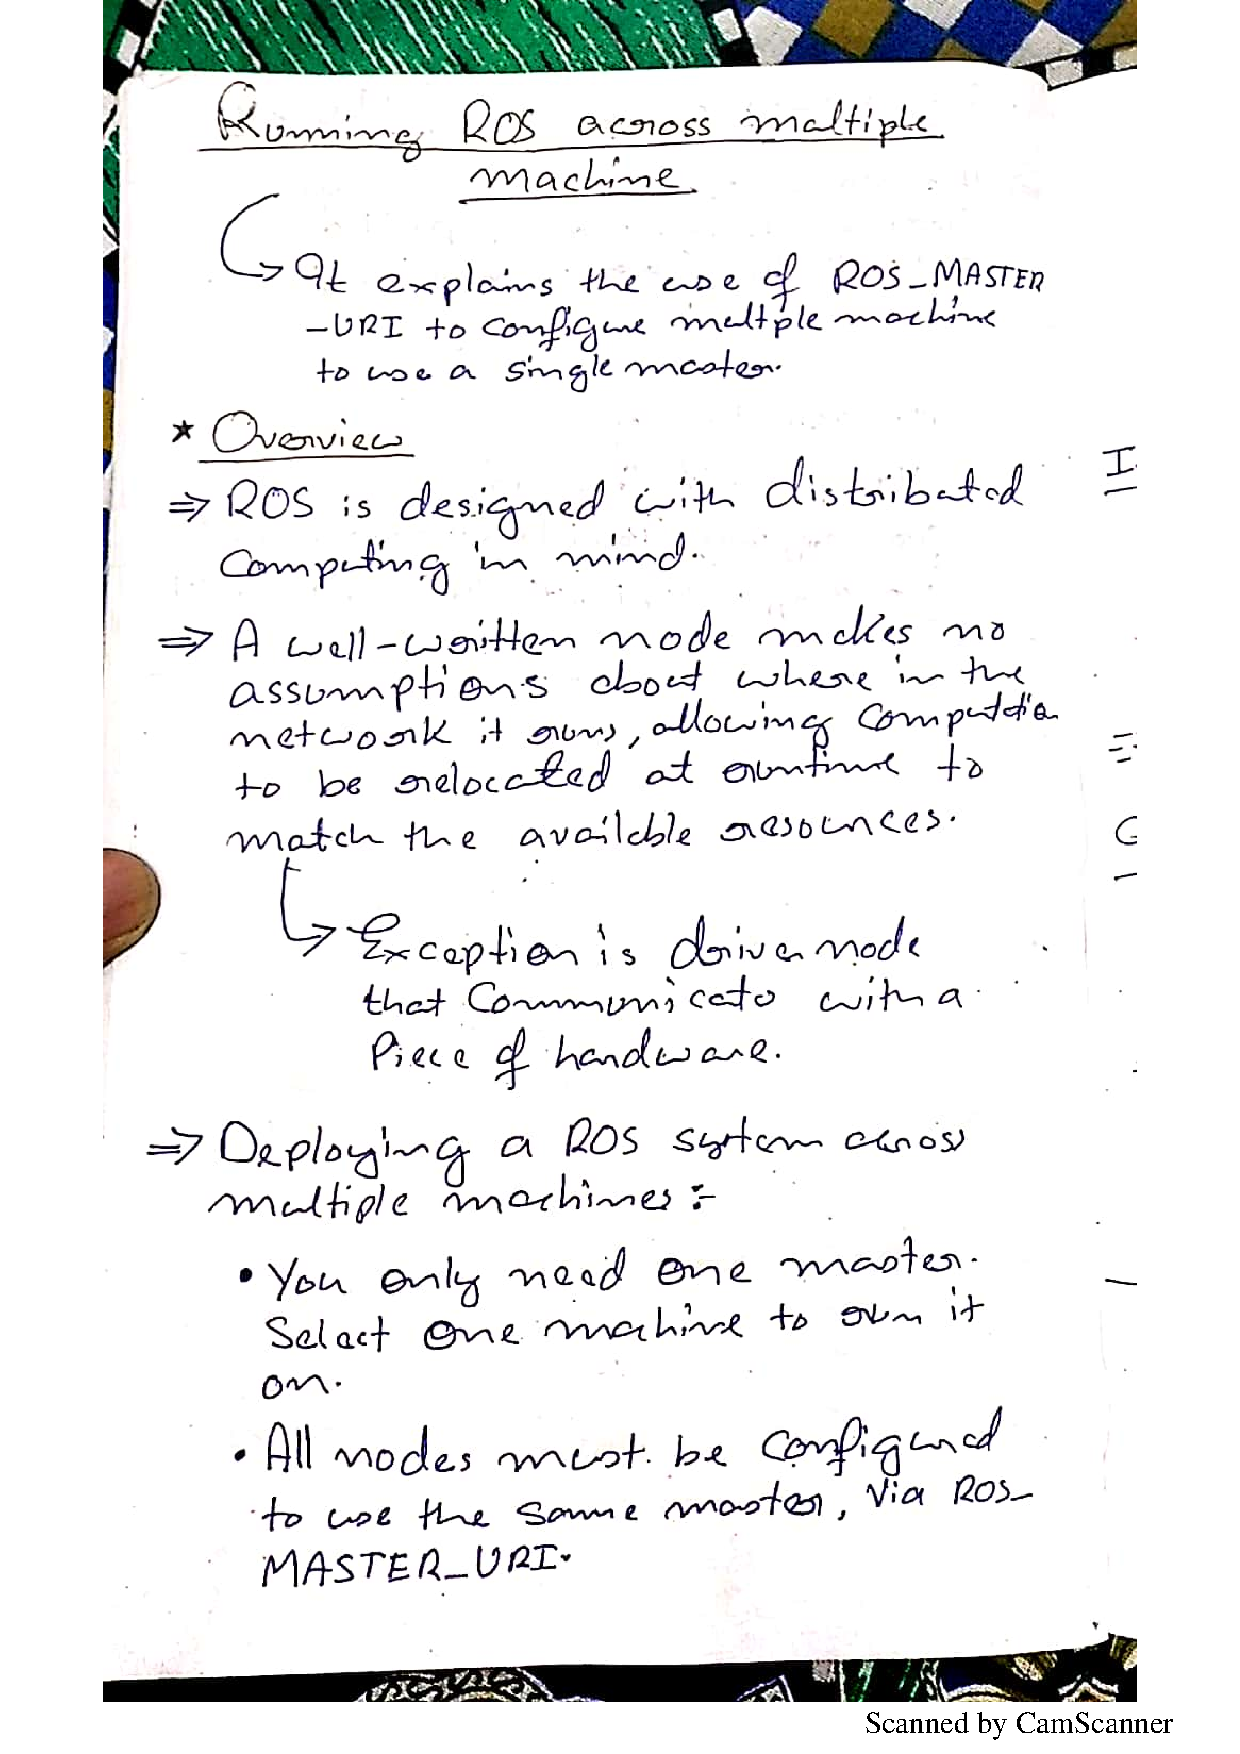
\includepdf[page=-]{./raw_files/29.pdf}

\chapter{RPLiDAR}
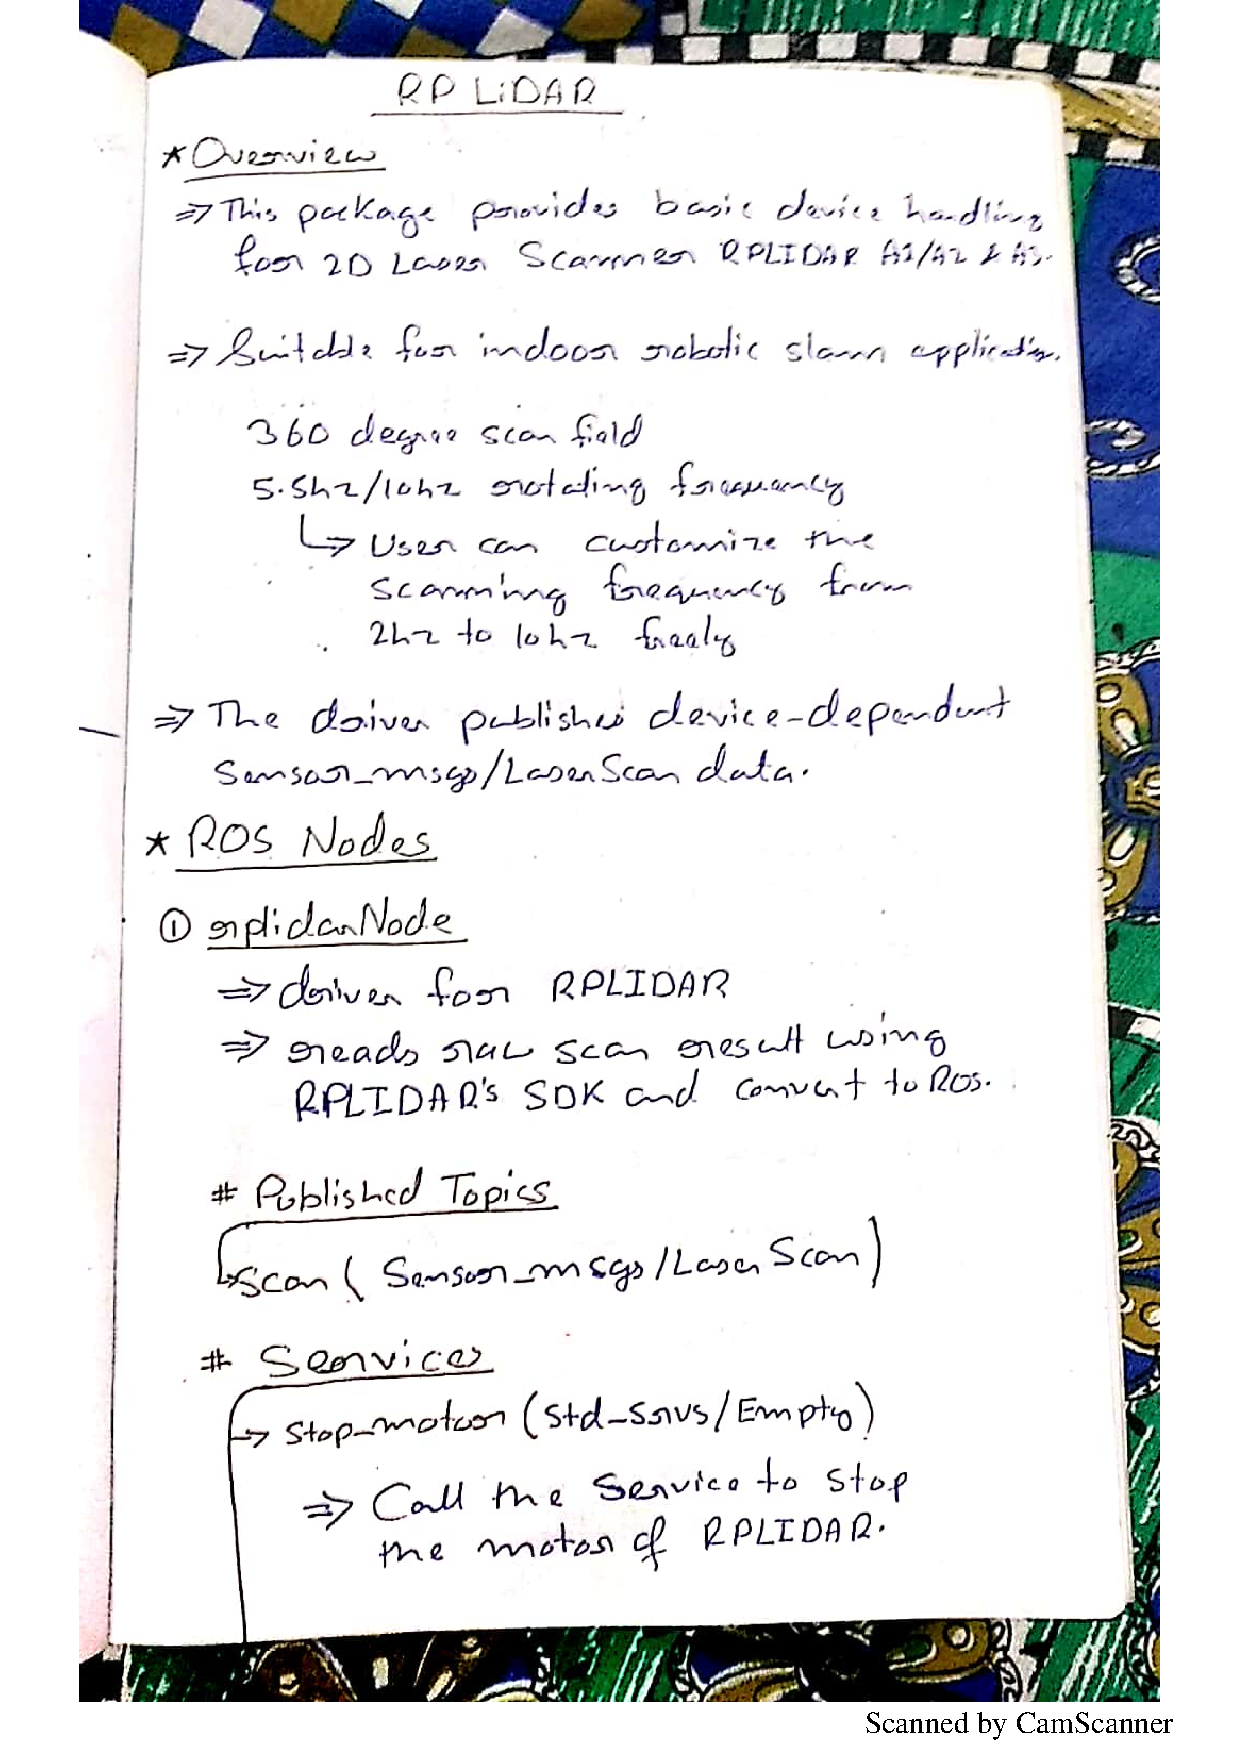
\includepdf[page=-]{./raw_files/30.pdf}

\chapter{Gmapping}
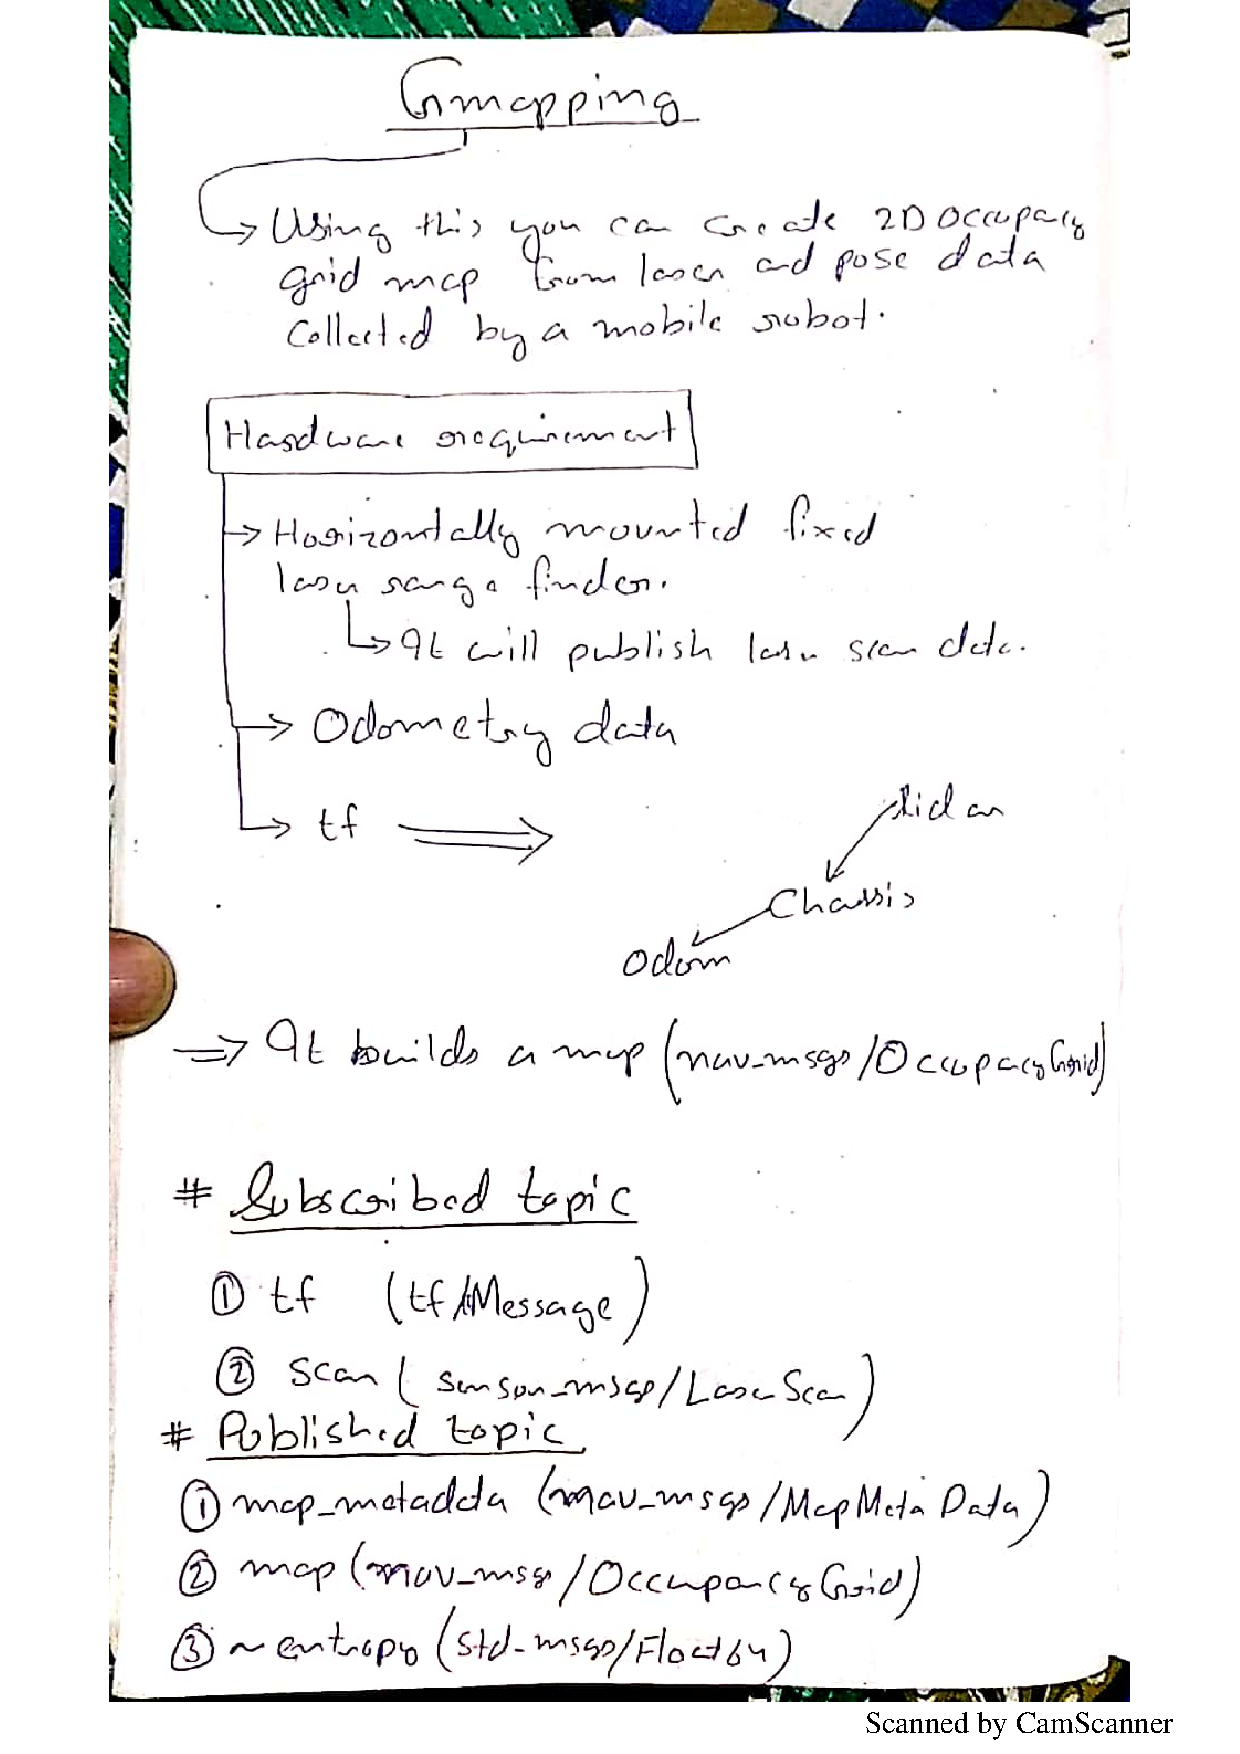
\includepdf[page=-]{./raw_files/31.pdf}

\chapter{Map Server}
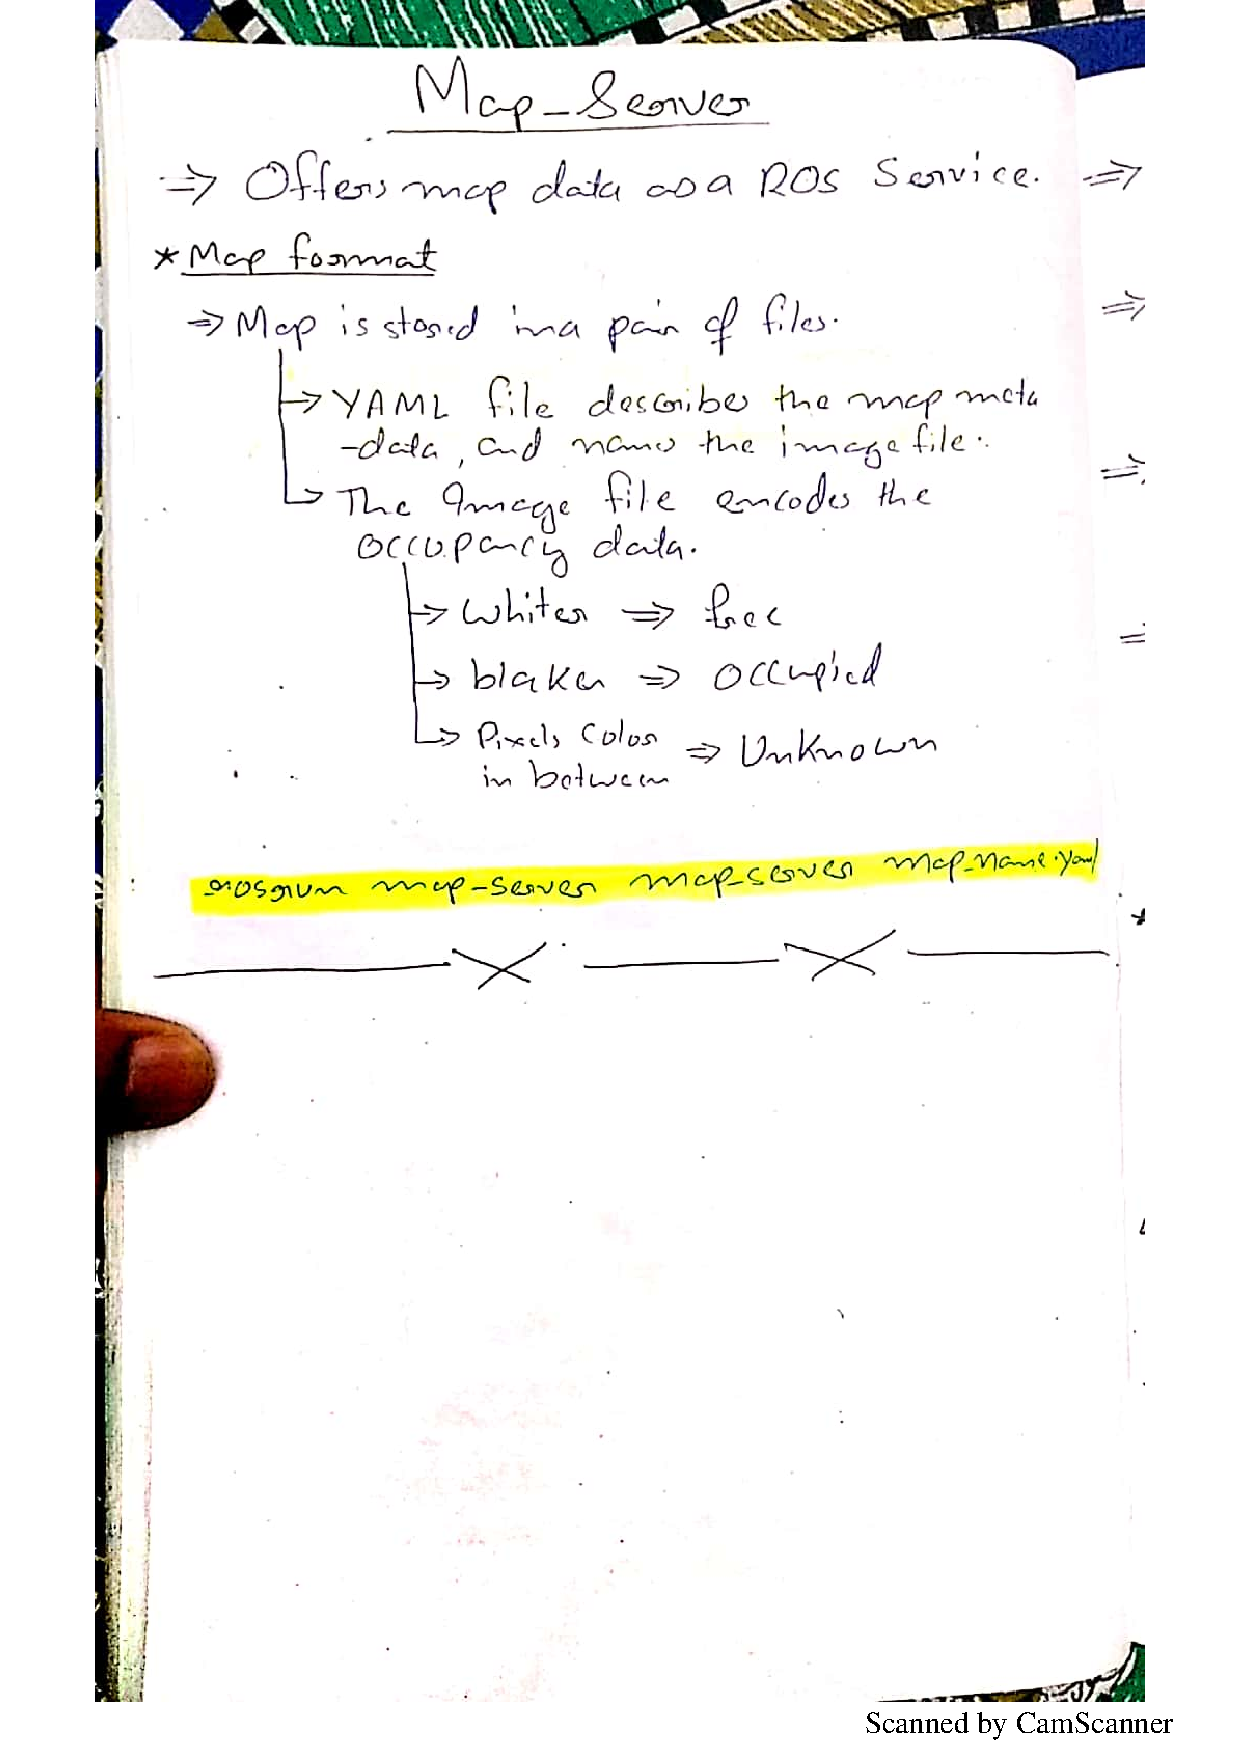
\includepdf[page=-]{./raw_files/32.pdf}

\chapter{AMCL}
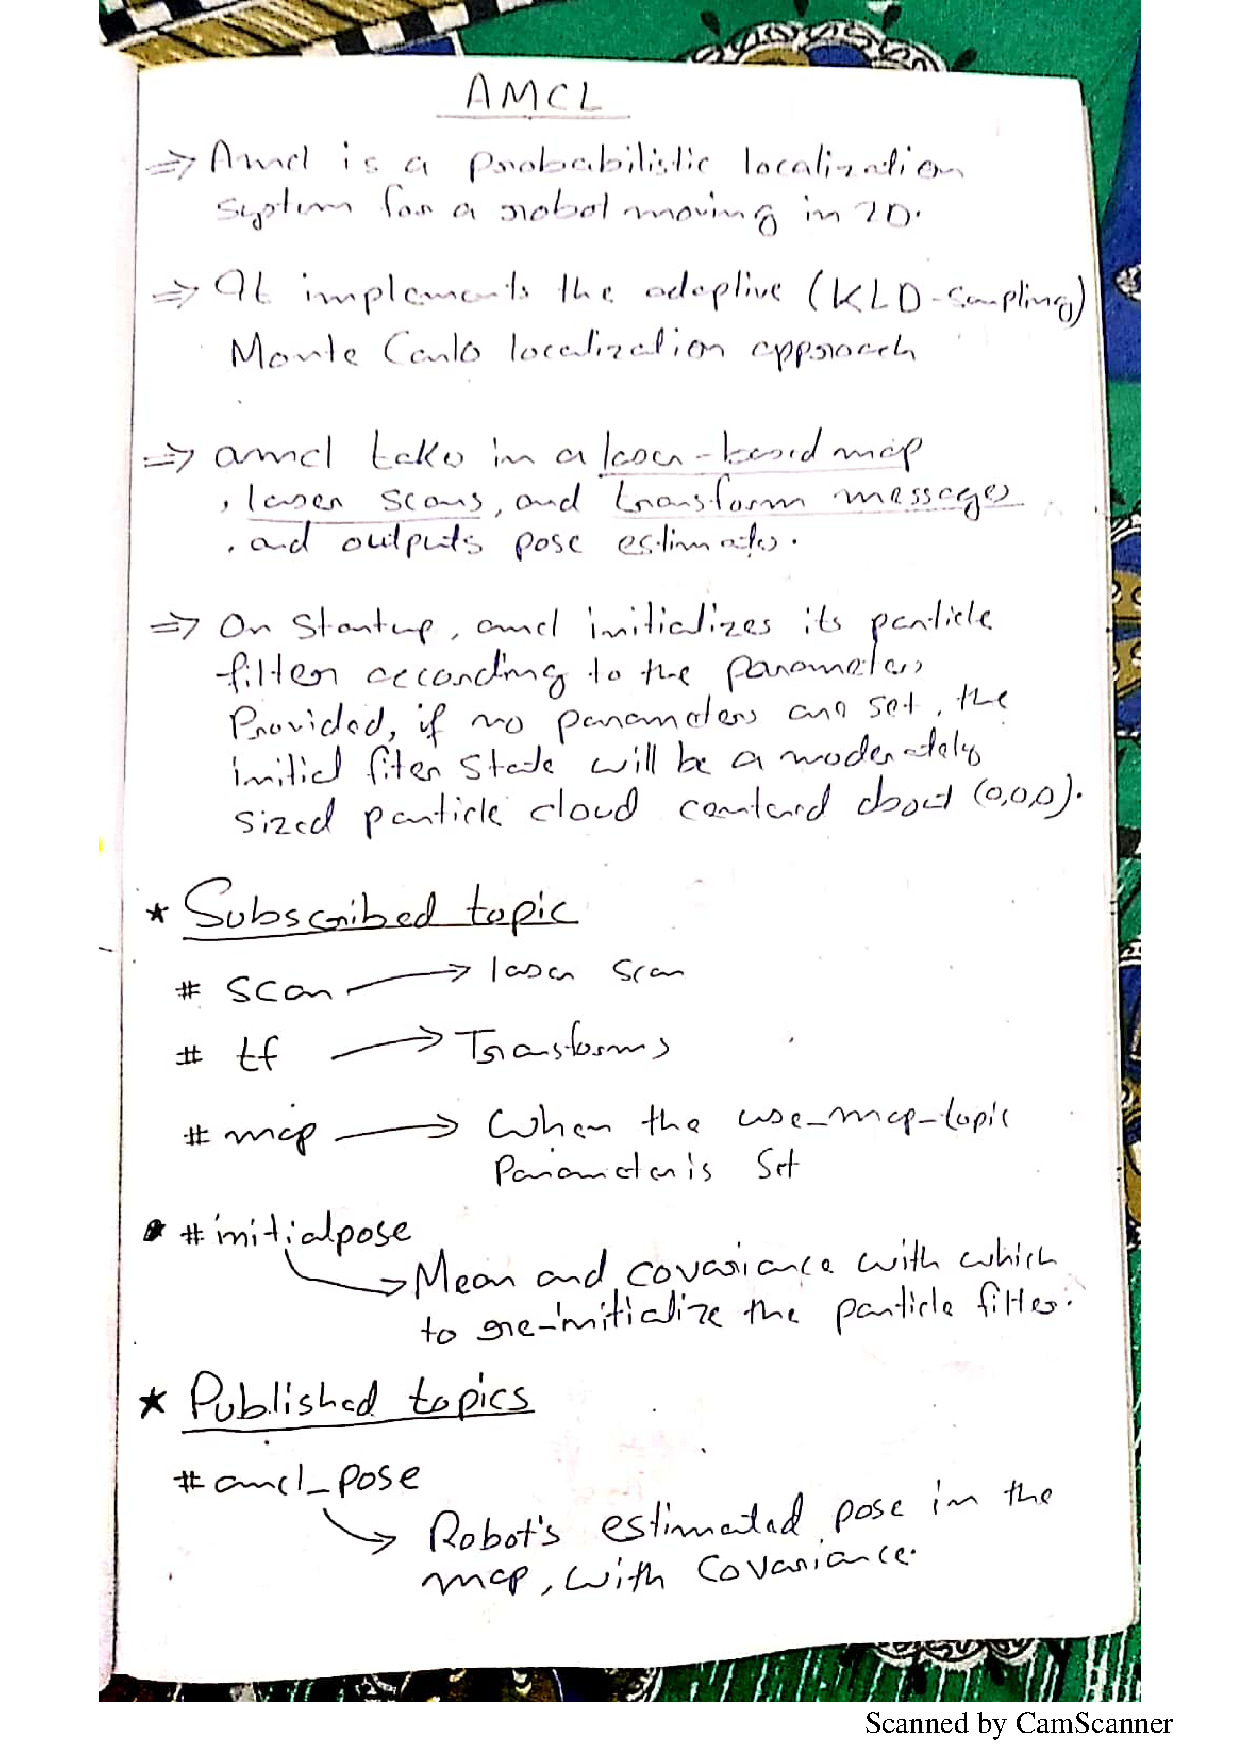
\includepdf[page=-]{./raw_files/33.pdf}


\end{document}